%  Thesis for Xiaolei Chen

\documentclass[12pt]{report}
\usepackage{thesis}
\usepackage{graphicx}
\usepackage{amsmath}
\usepackage{amssymb}		% to see postscript files
\usepackage{doublespace}

\usepackage[dvips]{epsfig}
\usepackage{multirow}
\usepackage{color}
\usepackage{listings}
\usepackage{verbatim}
\usepackage{epstopdf}
\usepackage{subcaption}
\usepackage{mathrsfs}
\DeclareGraphicsExtensions{.pdf,.png,.jpg,.eps}

\def\doublespace{1.66}		% 1.66 for double spacing with 12pt
\def\singlespace{1.00}		% 1.00 for single spacing
\def\defaultspace{\doublespace}	% adjust spacing factor

%
% Color
%
\definecolor{codegreen}{rgb}{0,0.6,0}
\definecolor{codegray}{rgb}{0.5,0.5,0.5}
\definecolor{codepurple}{rgb}{0.58,0,0.82}
\definecolor{backcolour}{rgb}{0.95,0.95,0.92}

\lstdefinestyle{mystyle}{
    backgroundcolor=\color{backcolour},
    commentstyle=\color{codegreen},
    keywordstyle=\color{magenta},
    numberstyle=\tiny\color{codegray},
    stringstyle=\color{codepurple},
    basicstyle=\footnotesize,
    breakatwhitespace=false,
    breaklines=true,
    captionpos=b,
    keepspaces=true,
    numbers=left,
    numbersep=5pt,
    showspaces=false,
    showstringspaces=false,
    showtabs=true,
    tabsize=2,
    frame=\shadowbox
}
\lstset{style=mystyle}
				

%\newcommand{\RR}{\mathcal{R}}
\newcommand{\posdisc}{\delta}
\newcommand{\widebar}[1]{\bar{#1}}
\newcommand{\skspd}{s}
\newcommand{\RR}{\mathrm{I\!R\!}}

\newcommand{\rarefset}{\mathcal{R}}
\newcommand{\shockset}{\mathcal{S}}
\newcommand{\waveset}{\mathcal{W}}
\newcommand{\Lstar}{\mathcal{L}^*}
\newcommand{\Leps}{\mathcal{L}_{\epsilon}}
\newcommand{\fan}{\mathcal{F}}
\newcommand{\lls}{l^*}
\newcommand{\lle}{l}
\newcommand{\gm}{\gamma}
\newcommand{\al}{\alpha}
\newcommand{\lbd}{\lambda}
\newcommand{\bt}{\beta}
\newcommand{\zt}{\zeta}
\newcommand{\fal}[2]{\{ \alpha(k) \}_{k={#1}}^{#2} }
\newcommand{\fbt}[2]{\{ \beta(k)  \}_{k={#1}}^{#2} }
\newcommand{\fgm}[2]{\{ \gamma(k) \}_{k={#1}}^{#2} }
\newcommand{\BigO}[1]{\mathcal{O}({#1})}
\newcommand{\ka}{k_{\alpha}}
\newcommand{\sa}{\sigma_{\alpha}}
\newcommand{\qp}{q^+_i}
\newcommand{\qm}{q^-_i}
\newcommand{\qmk}{q^-_{k_{\alpha}}}
\newcommand{\qpk}{q^+_{k_{\alpha}}}
\newcommand{\xa}{\dot{x}_{\alpha}}
\newcommand{\quadratic}{\lfloor \sigma_{\alpha} \rfloor^2}
\newcommand{\cubic}{\lfloor \sigma_{\alpha} \rfloor^3}

\newcommand{\wv}{\alpha}
\newcommand{\wvII}{\beta}
\newcommand{\disc}{\delta}
\newcommand{\disconset}{\mathcal{D}}
\newcommand{\kdisc}{k_{\delta}}
\newcommand{\kwv}{k_{\alpha}}
\newcommand{\up}{u^+}
\newcommand{\um}{u^-}
\newcommand{\xd}{\dot{x}}
\newcommand{\Sgn}{\operatorname{sign}}
\newcommand{\vect}[1]{\mathbf{#1}}


\newtheorem{definition}{Definition}[section]  
\newtheorem{notation}{Notation}[section]  
\newtheorem{theorem}{Theorem}[section]
\newtheorem{lemma}{Lemma}[section]
\newtheorem{proposition}[lemma]{Proposition}
\newtheorem{hyp}{Hypothesis}[section]
			% include personal macros here
%%%% my notation
\parindent = 5ex

\newcommand\ams{Department of Applied Mathematics and Statistics}
\newcommand\bnl{Center for Data Intensive Computing\\Brookhaven National Laboratory}

\newcommand{\half}{\mathchoice
 {\frac{1}{2}} {1/2} {\frac{1}{2}} {1/2}}

\newcommand{\quarter}{\mathchoice
 {\frac{1}{4}} {1/4} {\frac{1}{4}} {1/4}}
                             
\newcommand{\ud}{\mathrm{d}}

%%%% end of my notation

%
\newcommand{\doublespacing}{\renewcommand{\baselinestretch}{1.66}\normalsize}
\newcommand{\singlespacing}{\renewcommand{\baselinestretch}{1.00}\normalsize}
\newcommand{\beq}{\begin{equation}}
\newcommand{\eeq}{\end{equation}}
\newcommand{\bea}{\begin{eqnarray}}
\newcommand{\eea}{\end{eqnarray}}
%
% TODO enviroment
\newcommand{\todo}[1]{[*** TO DO: #1 ***]}
\newenvironment{TODO}
 {\goodbreak\medskip\par\noindent
   TO DO:\par\noindent$\overline{*****}$\begin{itemize}}
    {\end{itemize}\par\noindent$\underline{*****}$\medskip}
%
% Macros for noninteracting cluster theory and vapor condensation:
% 
\newcommand{\dissty}{\displaystyle}
\newcommand{\scrsty}{\scriptstyle}
%
% cross-referencing
%\newcommand{\eqref}[1]{(\ref{#1})}
\newcommand{\FronTierp}{\textit{\hbox{Fron\hspace{-2pt}T\hspace{-1pt}ier++\hspace{4pt}}}}
\newcommand{\Equation}[1]{Equation~\eqref{#1}}
\newcommand{\Equations}[1]{Equations~\eqref{#1}}
\newcommand{\Eqn}[1]{Eq.~\eqref{eqn:#1}}
\newcommand{\Eqs}[1]{Eqs.~\eqref{#1}}
\newcommand{\Eqsthru}[2]{Eqs.~\eqref{#1}--\eqref{#2}}
\newcommand{\Eqand}[2]{Eqs.~\eqref{#1} and~\eqref{#2}}
\newcommand{\Equationsand}[2]{Equations~\eqref{#1} and~\eqref{#2}}
\newcommand{\Eqor}[2]{Eq.~\eqref{#1} or~\eqref{#2}}
\newcommand{\Fig}[1]{Fig.~\ref{fig:#1}}
\newcommand{\Figure}[1]{Figure.~\ref{#1}}
\newcommand{\Figs}[2]{Figs.~\ref{#1}--\ref{#2}}
\newcommand{\Sec}[1]{Sec.~\ref{Sec:#1}}
\newcommand{\Secs}[2]{Secs.~\ref{#1}--\ref{#2}}
\newcommand{\Chap}[1]{Chapter~\ref{Chap:#1}}
\newcommand{\Tab}[1]{Table~\ref{tab:#1}}
\newcommand{\old}[1]{
{}}

%
\newcommand{\vaporliquid}{vapor-liquid{ }}
%
% units
\newcommand{\degC}{\mbox{$^\circ$C}{}}
\newcommand{\degF}{\mbox{$^\circ$F}{}}
\newcommand{\bars}{\mbox{bars}{}}
\newcommand{\meters}{\mbox{m}{}}
\newcommand{\grams}{\mbox{g}{}}
\newcommand{\mm}{\mbox{mm}{}}
\newcommand{\cm}{\mbox{cm}{}}
\newcommand{\nm}{\mbox{nm}{}}
%\newcommand{\um}{\mbox{$\mu$m}{}}
\newcommand{\secs}{\mbox{s}{}}
\newcommand{\msec}{\mbox{ms}{}}
\newcommand{\usec}{\mbox{$\mu$s}{}}
\newcommand{\nsec}{\mbox{ns}{}}
\newcommand{\cmpers}{\mbox{cm/s}{}}
\newcommand{\mpers}{\mbox{m/s}{}}
\newcommand{\ergperg}{\mbox{erg/g}{}}
\newcommand{\ccperg}{\mbox{cm$^3$/g}{}}
\newcommand{\gpercc}{\mbox{g/cm$^3$}{}}
\newcommand{\gpercmsq}{\mbox{g/cm$^2$}{}}
\newcommand{\ergpergK}{\mbox{erg/g-K}{}}
\newcommand{\nperccpers}{\mbox{nuclei/cm$^3$-s}{}}
\newcommand{\percc}{\mbox{/cm$^3$}{}}
\newcommand{\perccpers}{\mbox{cm$^{-3}$s$^{-1}$}{}}
%
% numeral adjectives
\newcommand{\St}{{\mbox{\small st}}}
\newcommand{\Nd}{{\mbox{\small nd}}}
\newcommand{\Rd}{{\mbox{\small rd}}}
\newcommand{\Th}{{\mbox{\small th}}}
%
% Latin abbreviations
\newcommand{\etc}{{\em etc}}
\newcommand{\ie}{{\em i.e., }}
\newcommand{\Ie}{{\em I.e., }}
\newcommand{\cf}{{\em cf.~}}
\newcommand{\etal}{{\em et~al.}}
\newcommand{\eg}{{\em e.g., }}
\newcommand{\viz}{{\em viz., }}
\newcommand{\vs}{{\em vs.~}}
\newcommand{\via}{{\em via }}
\newcommand{\viceversa}{{\em vice-versa}}
%
% For the following, math mode is assumed.
%
% Regular derivatives
\newcommand{\oderiv}[2]{{\displaystyle \frac{d #1}{d #2}}}
\newcommand{\pderiv}[2]{{\displaystyle \frac{\partial {#1}}{\partial {#2}}}}
\newcommand{\pderivc}[3]{{\displaystyle \left(\pderiv{#1}{#2}\right)_{#3}}}
%
% Thermodynamic derivatives
\newcommand{\thermoDeriv}[3]{{\displaystyle \left(\frac{\partial {#1}}{\partial {#2}}\right)_{#3}}}
\newcommand{\thermoDerivInline}[3]{{\displaystyle \left(\partial {#1}/\partial {#2}\right)_{#3}}}
\newcommand{\thermoTwoDeriv}[3]{{\displaystyle \left(\frac{\partial^2 {#1}}{\partial {#2}^2}\right)_{#3}}}
\newcommand{\thermoTwoDerivInline}[3]{{\displaystyle \left(\partial^2
{#1}/\partial {#2}^2\right)_{#3}}}
%
% Ways to display fractions with the proper size
\newcommand{\sfrac}[2]{{\textstyle \frac{#1}{#2}}}
\newcommand{\bfrac}[2]{{\displaystyle \frac{#1}{#2}}}
%
%
%%%%%%%%%%%%%%%%%%%%%%%%%%%%  Notation %%%%%%%%%%%%%%%%%%%%%%%%%%%%%%
%
\newcommand{\D}{\mathcal{D}}
\newcommand{\Dtilde}{\tilde{\mathcal{D}}}
% Riemann problem notation 
\newcommand{\Jfr}{J_{\mbox{\scriptsize fr}}}
\newcommand{\Jss}{J_{\mbox{\scriptsize ss}}}
\newcommand{\Mfr}{M_{\mbox{\scriptsize fr}}}
\newcommand{\Mss}{M_{\mbox{\scriptsize ss}}}
\newcommand{\Ifr}{I_{\mbox{\scriptsize fr}}}
\newcommand{\Iss}{I_{\mbox{\scriptsize ss}}}
\newcommand{\ufr}{u_{\mbox{\scriptsize fr}}}
\newcommand{\uss}{u_{\mbox{\scriptsize ss}}}
\newcommand{\Pfr}{P_{\mbox{\scriptsize fr}}}
\newcommand{\Pss}{P_{\mbox{\scriptsize ss}}}
\newcommand{\Dfr}{D_{\mbox{\scriptsize fr}}}
\newcommand{\Dss}{D_{\mbox{\scriptsize ss}}}
%
% Important cluster and droplet sizes and rates
\newcommand{\ivapor}{i_v}
\newcommand{\imax}{i_{\max}}
\newcommand{\icrit}{i_*}
\newcommand{\mcrit}{m_*}
\newcommand{\rcrit}{r_*}
\newcommand{\idrop}{i_o}
\newcommand{\mdrop}{m_o}
\newcommand{\rdrop}{r_o}
\newcommand{\dsize}{i_d}
\newcommand{\dmass}{m_d}
\newcommand{\dradius}{r_d}
\newcommand{\dtemp}{T_d}
\newcommand{\igrowth}{\Omega_i}
\newcommand{\mgrowth}{\Omega_m}
\newcommand{\rgrowth}{\Omega_r}
\newcommand{\ratevars}{{\bf \Lambda}}
\newcommand{\ratecoeffs}{{\bf R}}
\newcommand{\corrfac}{\Gamma}
%
% Reduced and dimensionless variables
\newcommand{\Phat}{\widehat{P}}
\newcommand{\Vhat}{\widehat{V}}
\newcommand{\That}{\widehat{T}}
\newcommand{\Stilde}{\widetilde{S}}
\newcommand{\Etilde}{\widetilde{E}}
\newcommand{\CVtilde}{\widetilde{C}_V}
\newcommand{\Btilde}[1]{\widetilde{B}_{#1}}
%
\newcommand{\Tref}{T_{\mbox{\scriptsize ref}}}
\newcommand{\Trefscr}{T_{\mbox{\scriptsize ref}}}
\newcommand{\Reff}{R_{\mbox{\scriptsize eff}}}
\newcommand{\State}{{\bf U}}
\newcommand{\state}{U}
\newcommand{\Flux}{{\bf f}}
\newcommand{\Numflux}{{\bf F}}
\newcommand{\massflux}{{\cal M}}
\newcommand{\entropy}{S}
\newcommand{\sat}{{\cal S}}
\newcommand{\Sonebar}{\overline{\cal S}_1}
\newcommand{\Sonehat}{\widehat{\cal S}_1}
\newcommand{\Hug}{{\cal H}}
\newcommand{\Kn}{\mbox{\em Kn}}
\newcommand{\smallKn}{\mbox{\small\em Kn}}
\newcommand{\QN}[2]{\frac{Q_{#1}^{#2}}{{#2}!}}
\newcommand{\sumto}[2]{\sum_{{#1}=1}^{#2}}
\newcommand{\sumtoinf}[1]{\sum_{{#1}=1}^{\infty}}
\newcommand{\fprime}[1]{f_{#1}^\prime}
\newcommand{\Nbar}[1]{\overline{N}_{#1}}
\newcommand{\nbar}[1]{\overline{n}_{#1}}
\newcommand{\mubar}[1]{\overline{\mu}_{#1}}
\newcommand{\Gbar}{\overline{G}}
\newcommand{\Cbar}[1]{\overline{C}_{#1}}
\newcommand{\ubar}{\overline{u}}
\newcommand{\muo}[1]{\mu_{#1}^{o}}
\newcommand{\muos}[1]{\mu_{#1,s}^{o}}
\newcommand{\nis}[1]{n_{#1,s}}
\newcommand{\licubed}{\lambda_{i}^{3}}
%
\newcommand{\nhat}[1]{\widehat{n}_{#1}}
\newcommand{\Chat}[1]{\widehat{C}_{#1}}
\newcommand{\expten}[1]{\cdot 10^{#1}}
%
% Formation energies
\newcommand{\dG}[1]{\Delta G_{#1}}
\newcommand{\dGs}[1]{\Delta G_{#1,s}}
\newcommand{\dGhat}[1]{\Delta\widehat{G}_{#1}}
%
% Nucleation notation
\newcommand{\Jminus}[1]{J_{#1-{\scriptscriptstyle 1/2}}}
\newcommand{\Jplus}[1]{J_{#1+{\scriptscriptstyle 1/2}}}
\newcommand{\JminusInline}[1]{J_{#1-1/2}}
\newcommand{\JplusInline}[1]{J_{#1+1/2}}
\newcommand{\timelag}[1]{\tau_{#1}}
\newcommand{\zel}{Z_{\icrit}}
%
% substances
\newcommand{\noctane}{\mbox{$n$-oc\-tane}{}}
\newcommand{\isooctane}{\mbox{iso-oc\-tane}{}}
\newcommand{\nhexane}{\mbox{$n$-hex\-ane}{}}
\newcommand{\nnonane}{\mbox{$n$-no\-nane}{}}
\newcommand{\ndecane}{\mbox{$n$-de\-cane}{}}
\newcommand{\nalkanes}{\mbox{$n$-al\-kanes}{}}
\newcommand{\nitrogen}{\mbox{N$_2$}{}}

\newtheorem{thm}{Theorem}[section]
\newtheorem{defn}[thm]{Definition}
\newtheorem{rem}[thm]{Remark}
\newtheorem{prop}[thm]{Proposition}
\newtheorem{lem}[thm]{Lemma}

\newcommand{\FronTier}{\textit{Fron\hspace{-2pt}T\hspace{-1pt}ier\hspace{2pt}}}

%From amsart.cls
%\newenvironment{pf}{\proof[\proofname]}{\endproof}
%\newenvironment{pf*}[1]{\proof[#1]}{\endproof}
 
%{\theoremstyle{plain}
%\newtheorem{thm}{Theorem}[section]
%\newtheorem{thm}{Theorem}
%\newtheorem{prop}[thm]{Proposition}
%\newtheorem{cor}[thm]{Corollary}
%\newtheorem{lem}[thm]{Lemma}
%\newtheorem{conj}[thm]{Conjecture}
%}
  
%{\theoremstyle{definition}
%\newtheorem{defn}[thm]{Definition}
%\newtheorem{assump}[thm]{Assumption}
%}
   
%{\theoremstyle{remark}
%\newtheorem{rem}{Remark}
%\newtheorem{notation}{Notation}
%\newtheorem{example}{Example}
%\newtheorem{summary}{Summary}
%}
%\renewcommand{\therem}{}
%\renewcommand{\theexample}{}
%\renewcommand{\thesummary}{}





\begin{document}

\pagestyle{prelim}		% puts roman numerals at bottom
\dissertation

\title{Closed-form Processor Equivalence And Scheduling Divisible Workloads From Multiple Sources In Regular, Toroidal And Hypercube Network}
\author{{\bf Junwei Zhang}}
\degree{Doctor of Philosophy}
\department{{\bf Applied Mathematics and Statistics}}
\month{\bf August}
\year{\bf 2018}

\maketitle

\begin{approval}
\member{\bf Thomas G. Robertazzi - Dissertation Advisor\\ 
Professor, \ece} 
\member{\bf Joseph S.B. Mitchell - Chairperson of Defense\\ 
Professor, \ams} 
\member{\bf Esther M. Arkin - Member\\ 
Professor, \ams} 
\member{\bf Yue Zhao -  Member\\
Professor, \ece}
\end{approval}
 
\begin{spacing}{\doublespace}
\begin{abstract}
This thesis considers two problems.  One problem is closed-form solutions for equivalence computation \cite{robertazzi1993processor} of divisible workload in a mesh networks and the other problem is scheduling divisible workloads from multiple sources in mesh networks of processors.  We propose a flow matrix closed-form equation to present the equivalence, which allows a characterization of the nature of minimal time solution and a simple method to determine when and how much load to distribute for processors.  In addition, we also propose a rigorous mathematics proof about the flow matrix optimal solution existence and unique.  Also, we propose the use of a reduced Manhattan distance Voronoi diagram algorithm (RMDVDA) to minimize the overall processing time of these workloads by taking advantage of the processor equivalence technique.  The user case studies with $10$ sources of workloads are presented to illustrate the general approach for multiple sources of workloads.  In the first phase, a Voronoi Manhattan distance diagram is used to obtain a network cluster division.  In the second phase, we propose an efficient algorithm to obtain near-optimal load distribution among processors represented by equivalent processors.  The algorithm minimizes the number of processors utilized.  Experimental evaluation through simulations demonstrates that a task can be finished in the same suboptimal time and yet save about $30\%$ of processor resources.  Further, the lower band of intuitive and heuristic algorithm is also investigated.
\end{abstract}
 
\begin{dedication}
\begin{center}
{\Large \it To my Parents and all loving ones}
\end{center}

\end{dedication}
 
\tableofcontents
\listoffigures
\listoftables
\end{spacing}

\begin{spacing}{\defaultspace}
\begin{acknowledgements}
Thank you for Professor Thomas G. Robertazzi who gives me strong academic and emotional support in the past hard time period.  
\end{acknowledgements}
\end{spacing}

%end of preliminary
		% preliminary text

\begin{spacing}{\defaultspace}	% adjust spacing

\pagestyle{body}	   % puts Arabic numbers at top
\chapter{Introduction}
\label{Chap:Intro}

Four chapters are organized as follows :
\begin{itemize}
\item A problem introduction, notation and definitions are shown in Chapter \uppercase\expandafter{\romannumeral2}. 

\item Chapter \uppercase\expandafter{\romannumeral3} considers about the regular network.
We take into account of the processor equivalence problem with front-end scenario and without front-end situation.  The sensitivity analysis is another topic.  Considering about the multi-source workload assignment problem, we propose a reduced Voronoi diagram assignment.

\item Chapter \uppercase\expandafter{\romannumeral4} presents the toroidal rectangle network situation.  We consider the closed-form of processor equivalence in unique load injection, in different injection positions, corner processor, boundary processor and inner grid processor, respectively.  The sensitivity analysis and multi-source assignment problem are also referred. 

\item Chapter \uppercase\expandafter{\romannumeral5} investigates the hypercube network situation. The front-end and without front-end assumption are discussed.  The sensitivity analysis is referred and the multi-source assignment in hypercube environment is also an interesting problem.

\item Chapter \uppercase\expandafter{\romannumeral6} figures out the conclusion and future work.
\end{itemize}

\newpage

        % Introduction
\chapter{Problem Description}
\label{Chap:Models}
\section{Problem Background}
In large-scale data intensive problems with geographically distributed resources,  load is generated from multiple sources\cite{moges2009grid} for a class of problems.  It is assumed that the problem representation can be divided amongst the processors.  Thus the problem representation is said to be ``divisible".  The processing of massive amounts of data on distributed and parallel networks is becoming more and more common.  The problem of minimizing the processing time of extensive loads originating from a multiplicity of sources and being processed on a multiplicity of nodes presents a challenge.  \\
In this chapter, the closed-form processor equivalence\cite{robertazzi1993processor}\cite{Liu_1schedulingdivisible} problem in the grid network of regular network and toroidal rectangle network is discussed.  Also, the multi-source workload assignment is also taken into account.

In this thesis, we investigate two problems. One is the processor equivalence.  The other one is scheduling divisible workloads from multiple sources in regular network \Fig{5t5}, toroidal rectangle network \Fig{torusnetwork} and hypercube network \Fig{hypercube}.\\

\begin{figure}[!ht]
\centering
\includegraphics[width=0.8\columnwidth]{figure/5t5.JPG}
\caption{A m*n regular network(m = 5,  n = 5)}
\label{fig:5t5}
\end{figure}

\begin{figure}[!ht]
\centering
\includegraphics[width=1\columnwidth]{figure/torusnetwork.jpg}
\caption{A toroidal rectangle network with grid unit cores}
\label{fig:torusnetwork}
\end{figure}

\begin{figure}[!ht]
\centering
\includegraphics[width=0.8\columnwidth]{figure/hypercube.jpg}
\caption{A hypercube network}
\label{fig:hypercube}
\end{figure}
\newpage 

\section{Definitions and Assumption}

\theoremstyle{definition}
\begin{definition}{Equal Computation}\\
Equal computation is a technique, which considers combining a cluster of processors as one whole processor to process the unit $1$ workload.
\end{definition}

The following assumptions are used throughout the paper:

\begin{itemize}
\item The virtual cut through \cite{kermani1979virtual} switching is used to transmit the assigned workload between processors.
\item For simply, we do not consider return communications.  
\item The communication delays are taken into consideration.  
\item The time costs of computation and communication are assumed to be linear function of the data size.  
\item The network environment is homogeneous, that is, all the processors have the same computation capacity.  The link speeds between any two unit cores are identical.   
\item The number of outgoing ports in each processor is limited.  In NOC(network on chip), the port number is fixed 4 or 5.  
\item The general graph's grid node's in-degree and out-degree is 4 or 5.  
\end{itemize}

The optimization objective functions are as follows :
\begin{itemize}
\item Equal computation : the problem's objective function is how to partition and schedule the workloads amongst the processors to get the minimum finish time.  
\item Multi-source assignment : how to finish the unit $1$ workload at the same time utilizing smaller processor.
\end{itemize}

To achieve the minimum solution is obtained by forcing the processors over a network to stop processing simultaneously.  Intuitively, this is because the solution could be improved by transfer load from some busy processor to idle ones.  

\subsection{Notions}
The following notations and definitions are utilized:
\begin{itemize}
\item $P_{i}$: The $i$th processor.   $0  \leq i \leq m*n-1$.  
\item $L_{i}$: The $i$th work load.   $1 \leq i \leq k$.  
\item $D_{i}$: The minimum number of hops from the processor $P_{i}$ to the data load injection $L$.  
\item $level_{i}$: The processors have $i$ minimum Manhattan distance to the data injection.
\item $\alpha_{0}$: The load fraction assigned to the root processor.  
\item $\alpha_{i}$: The load fraction assigned to the $i$th processor.  
\item $\omega_{i}$: The inverse computing speed on the $i$th processor.  
\item $\omega_{eq}$: The inverse computing speed on an equivalent node collapsed from a cluster of processors.  

\item $z_{i}$: The inverse link speed on the $i$th link.  
\item $T_{cp}$: Computing intensity constant.  The entire load is processed in $\omega_{i}T_{cp}$ on the $i$th processor.  

\item $T_{cm}$: Communication intensity constant.  The entire load is transmitted in $z_{i}T_{cm}$ seconds over the $i$th link.  
\item $T_{f, n}$: The finish time of the whole processor network.  Here $T_{f, n}$ is equal to $\omega_{eq}T_{cp}$.  

\item $T_{f, 0}$: The finish time for the entire divisible load solved on the root processor.  Here $T_{f, 0}$ is equal to $1 \times \omega_{0}T_{cp}$,  that is $\omega_{0}T_{cp}$.  

\item $\sigma = \frac{zT_{cm}}{\omega T_{cp}}$: The ratio between the communication speed to the computation speed,  $0 < \sigma < 1$ \cite{bharadwaj1996scheduling} \cite{hung2004switching}.  

\item In multi-source situation, $\sum_{i = 1}^{k} L_{i} = 1$
\item $\sum_{i = 0}^{m*n-1} \alpha_{i}= 1$
\item $Speedup = \frac{T_{f, 0}}{T_{f, n}}= \frac{\omega T_{cp}}{\alpha_{0}\omega T_{cp}} = \frac{1}{\alpha_{0}}$
\end{itemize}
\newpage

\chapter{Regular network}

\section{With Front-end Scenario}
In the front-end environment, the communication and the computation is executed simultaneously.  That is, upon receiving their respective load fractions,  the processors start processing their own workload and rely all the other fractions to the neighbor processors at the same time.  

First we consider about the $2*2$ regular network,  $2*n$ regular network.  After, we analyze a more general case $m*n$ regular network and obtain a general closed-form matrix presentation.  Finally, we give a key principle to address this type of question.  In addition, different data injection position, such as the corner, boundary and inner grid are also discussed.  

\subsection{Data Injection on The Corner Processor}
\subsubsection{2*2 Regular Network}
The $L$ is assigned on the corner processor $P_{0}$ \Fig{2t2}.  The whole task is tackled by four processors $P_{0}$, $P_{1}$, $P_{2}$, $P_{3}$ together.  

\begin{figure}[!ht]
\centering
\includegraphics[width=0.5\columnwidth]{figure/2t2.JPG}
\caption{The 2*2 regular network and the root processor is $P_{0}$}
\label{fig:2t2}
\end{figure}

The processor $P_{0}$, $P_{1}$ and $P_{2}$ start to process its respective fraction at the same time.  The processor $P_{3}$ starts to work until the $\alpha_{1}$ and $\alpha_{2}$ are completed transmission.  

According to the divisible load theory\cite{bharadwaj2003divisible}, we obtain the timing diagram \Fig{2t2d}.  

\begin{figure}[!ht]
\centering
\includegraphics[width=0.5\columnwidth]{figure/2t2d.JPG}
\caption{The timing diagram for 2*2 regular network and the root processor is $P_{0}$}
\label{fig:2t2d}
\end{figure}
Based on the timing diagram, we get a group of equations to deploy the fraction workload:
\\
\begin{empheq}[left=\empheqlbrace]
{align}
\alpha_{0} \omega T_{cp} = T_{f, m}\\
\alpha_{1} \omega T_{cp} = T_{f, m}\\
\alpha_{2} \omega T_{cp} = T_{f, m}\\
\alpha_{1}zT_{cm} + \alpha_{3}\omega T_{cp} = T_{f, m}\\
\alpha_{0} + \alpha_{1} + \alpha_{2} + \alpha_{3} = 1\\
\sigma = \frac{zT_{cm}}{\omega T_{cp}}\\
0 < \sigma < 1 \\
0 < \alpha_{0} \leq  1\\
0 \leq  \alpha_{1},  \alpha_{2},  \alpha_{3}  < 1
\end{empheq}
\\

The group of equations are represented by the matrix form:

\begin{equation}
{
\left[ \begin{array}{ccc}
1 & 2 & 1\\
1 & -1 & 0\\
0 & \sigma-1 & 1
\end{array} 
\right ]} \times \left[ \begin{array}{c}
\alpha_{0} \\
\alpha_{1} \\
\alpha_{3} 
\end{array} 
\right ] = \left[ \begin{array}{c}
1 \\
0 \\
0 
\end{array} 
\right ]
\end{equation}
The matrix is represented as $A \times \alpha = b$.  $A$ is named as \textbf{\textit{flow matrix}}.

Finally, the explicit solution is:
\begin{empheq}[left=\empheqlbrace]
{align}
\sigma = \frac{zT_{cm}}{\omega T_{cp}}\\
\alpha_{0} = \frac{1}{4- \sigma}\\
\alpha_{1} = \frac{1}{4- \sigma}\\
\alpha_{3} = \frac{1 - \sigma}{4- \sigma}
\end{empheq}
\\

The simulation result is illustrated:
\begin{figure}[!ht]
\centering
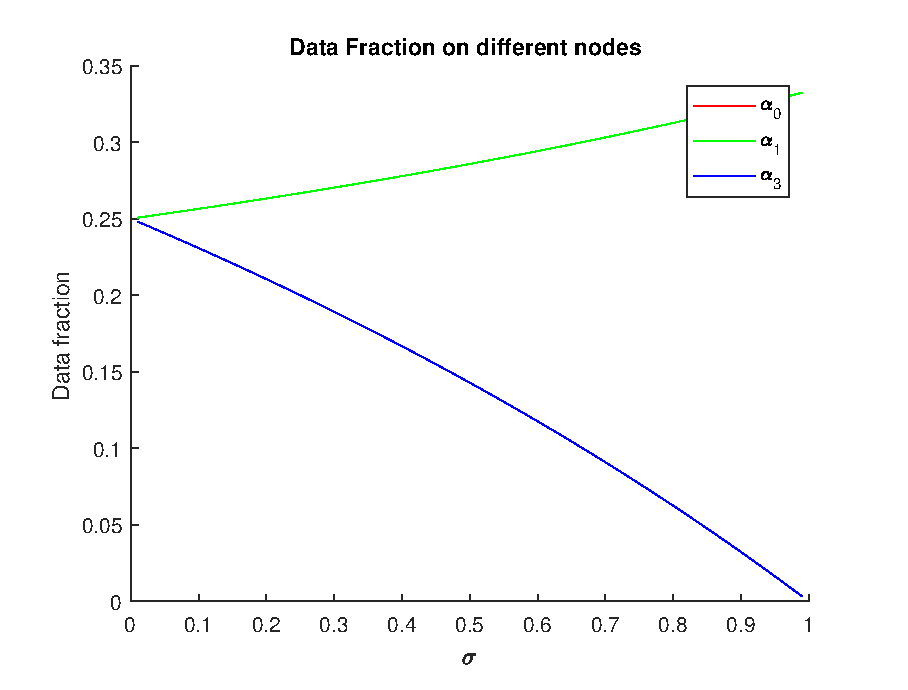
\includegraphics[width=1\columnwidth]{figure/2t2fraction}
\caption{2*2 regular network.  $\alpha_{0}$, $\alpha_{1}$, $\alpha_{2}$, $\alpha_{3}$ value curve}
\label{fig:2t2fraction}
\end{figure}
\newpage 

In \Fig{2t2fraction},  $P_{0}$, $P_{1}$, $P_{2}$ three processors have the same data fraction workload, so the curve of $\alpha_{0}$ and $\alpha_{1}$ coincide.  
The figure says that as $\sigma$ grows,  the value $\alpha_{3}$ drops.  In other words, as the communication capacity decreases, there is less data workload assigned to $P_{3}$.  Further, it means it will be economical to keep the load local on $P_{0}$ nor distribute it to other processors.  

The speedup is:
$$Speedup = \frac{T_{f, 0}}{T_{f, n}}= \frac{\omega T_{cp}}{\alpha_{0}\omega T_{cp}} = \frac{1}{\alpha_{0}} = 4- \sigma$$
\newpage 

\subsubsection{2*3 Regular Network}
In \Fig{2t3} regular network, $L$ happens on processor $P_{0}$.  There are $6$ processors to be processing.  
\begin{figure}[!ht]
\centering
\includegraphics[width=0.5\columnwidth]{figure/2t3.JPG}
\caption{The 2*3 regular network and the data injection happens on corner processor $P_{0}$}
\label{fig:2t3}
\end{figure}

Here $P_{0}$, $P_{1}$ and $P_{2}$ start processing at the same time.  Processor $P_{3}$ and $P_{4}$ start to work when they receive the data from processor $P_{1}$, $P_{2}$.  That is, $P_{3}$ and $P_{4}$ have to wait the fraction of $\alpha_{1}$ and $\alpha_{2}$ are transmitted completely.\\
The last processor $P_{5}$ starts to execute until the work load fraction $\alpha_{0}$, $\alpha_{1}$, $\alpha_{2}$, $\alpha_{3}$, $\alpha_{4}$ are transmitted completed.  According to the divisible load theory\cite{bharadwaj2003divisible}, we obtain the timing diagram \Fig{2t3d}.  

\newpage 
\begin{figure}[!ht]
\centering
\includegraphics[width=0.5\columnwidth]{figure/2t3d.JPG}
\caption{The timing diagram for a 2*3 regular network and the data injection happens on processor $P_{0}$}
\label{fig:2t3d}
\end{figure}

\newpage

The equations as follows:
\begin{empheq}
[left=\empheqlbrace]
{align}
\alpha_{0} \omega T_{cp} = T_{f, m}\\
\alpha_{1} \omega T_{cp} = T_{f, m}\\
\alpha_{2} \omega T_{cp} = T_{f, m}\\
\alpha_{1}zT_{cm} + \alpha_{3}\omega T_{cp} = T_{f, m}\\
\alpha_{2}zT_{cm} + \alpha_{4}\omega T_{cp} = T_{f, m}\\
(\alpha_{1} + \alpha_{3})zT_{cm} + \alpha_{5}\omega T_{cp} = T_{f, m}\\
\alpha_{0} + \alpha_{1} + \alpha_{2} + \alpha_{3} + \alpha_{4} + \alpha_{5} = 1\\
\sigma = \frac{zT_{cm}}{\omega T_{cp}}\\
0 < \sigma < 1 \\
0 < \alpha_{0} \leq 1\\
0 \leq \alpha_{1},  \alpha_{2},  \alpha_{3} , \alpha_{4} , \alpha_{5} < 1
\end{empheq}
\\

The flow matrix closed-form formula is:
\begin{equation}
{
\left[ \begin{array}{cccc}
1 & 2 & 2 & 1\\
1 & -1 & 0 & 0\\
0 & \sigma-1 & 1 & 0\\
0 & \sigma-1 & \sigma & 1
\end{array} 
\right ]} \times \left[ \begin{array}{c}
\alpha_{0} \\
\alpha_{1} \\
\alpha_{3} \\
\alpha_{5}
\end{array} 
\right ] = \left[ \begin{array}{c}
1 \\
0 \\
0 \\
0
\end{array} 
\right ]
\end{equation}
The explicit solution is:
\begin{empheq}[left=\empheqlbrace]
{align}
\sigma = \frac{zT_{cm}}{\omega T_{cp}}\\
\alpha_{0} = \frac{1}{\sigma^2- 4 \times \sigma + 6}\\
\alpha_{1} = \frac{1}{\sigma^2- 4 \times \sigma + 6}\\
\alpha_{3} = \frac{1 - \sigma}{\sigma^2 - 4 \times \sigma + 6}\\
\alpha_{5} = \frac{\sigma^2 - 2 \times \sigma + 1}{\sigma^2 - 4 \times \sigma + 6}
\end{empheq}
\\
The $\alpha$ calculation result are shown in \Fig{2t3fraction}.  
$P_{0}$,  $P_{1}$ have the same fraction so the curve of $\alpha_{0}$ and $\alpha_{1}$ coincide.  

\begin{figure}[!ht]
\centering
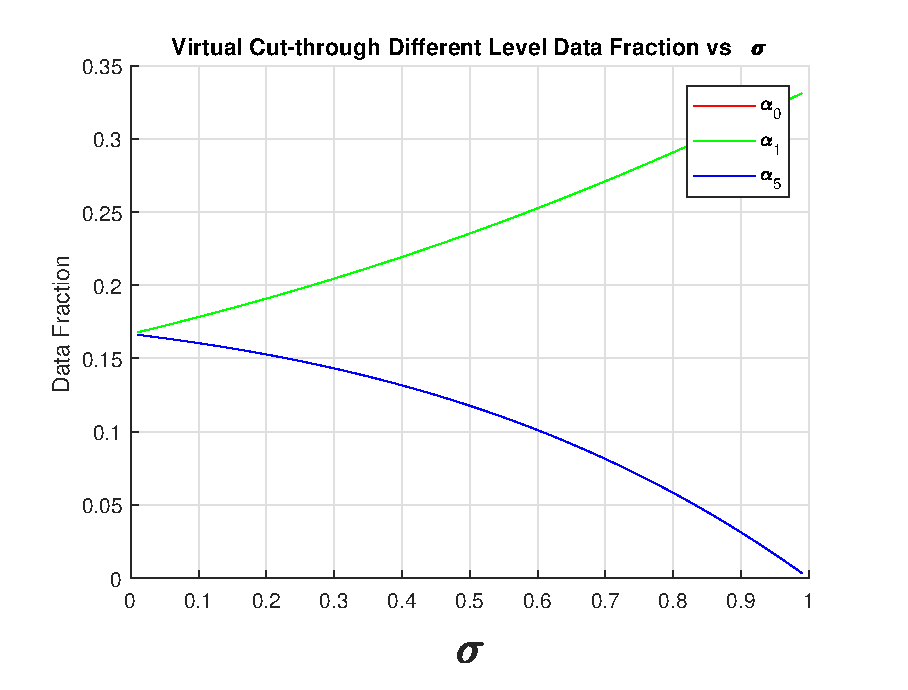
\includegraphics[width=1\columnwidth]{figure/2t3fraction.eps}
\caption{2*2 regular network.  $\alpha_{0}$, $\alpha_{1}$, $\alpha_{3}$, $\alpha_{5}$ data fraction value}
\label{fig:2t3fraction}
\end{figure}

\newpage
\subsubsection*{2*N Regular Network}
The $2*n$ \Fig{2t10} homogeneous regular network address $L_{1}$ at the same time and $L$ happens on $P_{0}$.  

\begin{figure}[!ht]
\centering
\includegraphics[width=0.6\columnwidth]{figure/2t10.JPG}
\caption{The 2*n (n = 10) regular network and the workload happens on $P_{0}$}
\label{fig:2t10}
\end{figure}
\newpage

Similarly to the analysis of \Fig{2t2d} and \Fig{2t3d},  the timing diagram for \Fig{2t10} is shown in \Fig{2t10d}

\begin{figure}[!ht]
\centering
\includegraphics[width=0.7\columnwidth]{figure/2t10d.jpg}
\caption{The timing diagram for 2*10 regular network and the data injection happens on $P_{0}$}
\label{fig:2t10d}
\end{figure}

The equations are presented as:
\begin{empheq}[left=\empheqlbrace]
{align}
\alpha_{0} \omega T_{cp} = T_{f, m}\\
\alpha_{1} \omega T_{cp} = T_{f, m}\\
\alpha_{2} \omega T_{cp} = T_{f, m}\\
\alpha_{1}zT_{cm} + \alpha_{3}\omega T_{cp} = T_{f, m}\\
\alpha_{2}zT_{cm} + \alpha_{4}\omega T_{cp} = T_{f, m}\\
(\alpha_{1} + \alpha_{3})zT_{cm} + \alpha_{5}\omega T_{cp} = T_{f, m}\\
\vdots \\
(\alpha_{1} + \alpha_{3} +\cdots + \alpha_{2 \times n - 1})zT_{cm} +\alpha_{2 \times n - 1} \omega T_{cp} = T_{f, m}\\
\alpha_{0} + \cdots + \alpha_{2 \times n - 1} = 1\\
\sigma = \frac{zT_{cm}}{\omega T_{cp}}\\
0 < \sigma < 1 \\
0 < \alpha_{0} \leq 1\\
0 \leq \quad \alpha_{1} \quad \alpha_{2} \quad  \cdots  \quad \alpha_{2 \times n - 1} < 1
\end{empheq}
\\

The flow matrix closed-form is shown:
\begin{equation}
{
\left[ \begin{array}{ccccccc}
1 & 2 & 2 & \cdots & 2 & 2 & 1\\
1 & -1 & 0 & \cdots& 0 & 0 & 0\\
0 & \sigma-1 & 1 & \cdots & 0 & 0 & 0 \\
0 & \sigma-1 & \sigma & 1 & 0 & \cdots & 0 \\
0 & \sigma-1 & \sigma & \sigma & 1 & 0 & 0 \\
\vdots & \vdots & \vdots  &   \vdots & \ddots & \ddots\\
0 & \sigma-1 & \sigma & \cdots & \sigma & \sigma & 1
\end{array} 
\right ]} \times \left[ \begin{array}{c}
\alpha_{0} \\
\alpha_{1} \\
\alpha_{3} \\
\alpha_{5} \\
\vdots \\
\alpha_{2 \times n - 3}\\
\alpha_{2 \times n - 1}
\end{array} 
\right ] = \left[ \begin{array}{c}
1 \\
0 \\
0 \\
0 \\
\vdots \\
0 \\
0
\end{array} 
\right ]
\end{equation}

According to the \textbf{\textit{Cramer's rule}},the explicit solution for the group of equations is:
\begin{empheq}[left=\empheqlbrace]
{align}
\alpha_{i} = \left |\frac{\det A^{\star}_{i}}{\det A}\right |
\end{empheq}
where $A^{\star}_{i}$ is the matrix formed by replacing the $i$-th column of A by the column vector b.\\
Especially,
\begin{equation}
{
A^{\star}_{0} = \left[ \begin{array}{ccccccc}
1 & 2 & 2 & \cdots & 2 & 2 & 1\\
0 & -1 & 0 & \cdots& 0 & 0 & 0\\
0 & \sigma-1 & 1 & \cdots & 0 & 0 & 0 \\
0 & \sigma-1 & \sigma & 1 & 0 & \cdots & 0 \\
0 & \sigma-1 & \sigma & \sigma & 1 & 0 & 0 \\
\vdots & \vdots & \vdots  &   \vdots & \ddots & \ddots\\
0 & \sigma-1 & \sigma & \cdots & \sigma & \sigma & 1
\end{array} 
\right ]}
\end{equation}

$$\alpha_{0} = \left |\frac{\det A^{\star}_{0}}{\det A} \right |$$
$$\det A^{\star}_{0} = -1$$

Finally, the speedup is:
$$Speedup = \frac{T_{f, 0}}{T_{f, n}}= \frac{\omega T_{cp}}{\alpha_{0}\omega T_{cp}} = \frac{1}{\alpha_{0}} =  \left|-\det A\right|$$.

Further, we prove the matrix $\det A \neq 0$. 
\renewcommand{\qedsymbol}{$\blacksquare$}

\begin{equation}
{
C = \left[ \begin{array}{cccccc}
-1 & 0 & \cdots& 0 & 0 & 0\\
\sigma-1 & 1 & \cdots & 0 & 0 & 0 \\
\sigma-1 & \sigma & 1 & 0 & \cdots & 0 \\
\sigma-1 & \sigma & \sigma & 1 & 0 & 0 \\
\vdots & \vdots & \vdots  &   \vdots & \ddots & \ddots\\
\sigma-1 & \sigma & \cdots & \sigma & \sigma & 1
\end{array} 
\right ]
}
\end{equation}

$C$ is a lower triangular matrix and the diagonal elements are not $0$.  So $C$ is non-degenerate, that is, the matrix is column linear independence.

After a series of column reduction and row reduction actions, we get
\begin{equation*}
     {A = \left[ \begin{array}{ccccccc}
1 & 2 & 2 & \cdots & 2 & 2 & 1\\
1 & -1 & 0 & \cdots& 0 & 0 & 0\\
0 & \sigma-1 & 1 & \cdots & 0 & 0 & 0 \\
0 & \sigma-1 & \sigma & 1 & 0 & \cdots & 0 \\
0 & \sigma-1 & \sigma & \sigma & 1 & 0 & 0 \\
\vdots & \vdots & \vdots  &   \vdots & \ddots & \ddots\\
0 & \sigma-1 & \sigma & \cdots & \sigma & \sigma & 1
\end{array} 
\right ]
\xrightarrow[\text{Reduction}]{\text{Column}}\\
\left[ \begin{array}{ccccccc}
1 & 0 & 0 & \cdots & 0 & 0 & 0\\
1 & -3 & -2 & \cdots& -2 & -2 & -1\\
0 & \sigma-1 & 1 & \cdots & 0 & 0 & 0 \\
0 & \sigma-1 & \sigma & 1 & 0 & \cdots & 0 \\
0 & \sigma-1 & \sigma & \sigma & 1 & 0 & 0 \\
\vdots & \vdots & \vdots  &   \vdots & \ddots & \ddots\\
0 & \sigma-1 & \sigma & \cdots & \sigma & \sigma & 1
\end{array} 
\right ]
}
\end{equation*}

\begin{equation*}
{\xrightarrow[\text{Reduction}]{\text{Row}}\\
\left[ \begin{array}{ccccccc}
1 & 0 & 0 & \cdots & 0 & 0 & 0\\
0 & -3 & -2 & \cdots& -2 & -2 & -1\\
0 & \sigma-1 & 1 & \cdots & 0 & 0 & 0 \\
0 & \sigma-1 & \sigma & 1 & 0 & \cdots & 0 \\
0 & \sigma-1 & \sigma & \sigma & 1 & 0 & 0 \\
\vdots & \vdots & \vdots  &   \vdots & \ddots & \ddots\\
0 & \sigma-1 & \sigma & \cdots & \sigma & \sigma & 1
\end{array} 
\right ]
}
\end{equation*}
Considering the matrix $\hat{C}$
\begin{equation}
{
\hat{C} = \left[ \begin{array}{cccccc}
-3 & -2 & \cdots& -2 & -2 & -1\\
\sigma-1 & 1 & \cdots & 0 & 0 & 0 \\
\sigma-1 & \sigma & 1 & 0 & \cdots & 0 \\
\sigma-1 & \sigma & \sigma & 1 & 0 & 0 \\
\vdots & \vdots & \vdots  &   \vdots & \ddots & \ddots\\
\sigma-1 & \sigma & \cdots & \sigma & \sigma & 1
\end{array} 
\right ]
}
\end{equation}
, which is still column linear independence.  Considering $0 < \sigma < 1$, the flow matrix is full rank. So $\det A \neq 0$.

After three user cases' investigation, we find a crucial rule:
\textbf{$$\forall D_{i} = D_{j}, \quad then \quad \alpha_{i} = \alpha_{j},  \quad  0 \leq i,  j \leq m*n-1$$}

\newpage

\subsubsection*{m*n Regular Network}
Considering a general $m*n$ regular network,  such as \Fig{3t8} \Fig{5t5}.  

\begin{figure}[!ht]
\centering
\includegraphics[width=0.55\columnwidth]{figure/3t8.JPG}
\caption{3*8 regular network.  The data injection position is $P_{0}$}
\label{fig:3t8}
\end{figure}

\begin{figure}[!ht]
\centering
\includegraphics[width=0.55\columnwidth]{figure/5t5.JPG}
\caption{5*5 regular network.  The data injection position is $P_{0}$}
\label{fig:5t5}
\end{figure}

Utilizing the rule, we obtain the closed-form flow matrix equations for \Fig{3t8}:
\begin{equation}
{
\left[ \begin{array}{cccccccccc}
1 & 2 & 3 & 3 & 3 & 3 & 3 & 3 & 2 & 1\\
1 & -1 & 0 & 0 & 0 & 0 & 0 & 0 & 0 & 0\\
0 & \sigma-1 & 1 & 0 & 0 & 0 & 0 & 0 & 0 & 0 \\
0 & \sigma-1 & \sigma & 1 & 0 & 0 & 0 & 0 & 0 & 0 \\
0 & \sigma-1 & \sigma & \sigma & 1 & 0 & 0 & 0 & 0 & 0\\
0 & \sigma-1 & \sigma & \sigma & \sigma & 1 & 0 & 0 & 0 & 0\\
0 & \sigma-1 & \sigma & \sigma & \sigma & \sigma & 1 & 0 & 0 & 0\\
0 & \sigma-1 & \sigma & \sigma & \sigma & \sigma & \sigma & 1 & 0 & 0\\
0 & \sigma-1 & \sigma & \sigma & \sigma & \sigma & \sigma & \sigma & 1 & 0\\
0 & \sigma-1 & \sigma & \sigma & \sigma & \sigma & \sigma & \sigma & \sigma & 1 \\
\end{array} 
\right ]} \times \left[ \begin{array}{c}
\alpha_{0} \\
\alpha_{1} \\
\alpha_{3} \\
\alpha_{6} \\
\alpha_{9} \\
\alpha_{12}\\
\alpha_{15}\\
\alpha_{18}\\
\alpha_{21}\\
\alpha_{23}
\end{array} 
\right ] = \left[ \begin{array}{c}
1 \\
0 \\
0 \\
0 \\
0 \\
0 \\
0 \\
0 \\
\vdots \\
0
\end{array} 
\right ]
\end{equation}

Also, the flow matrix equations for \Fig{5t5}:
\begin{equation}
{
\left[ \begin{array}{ccccccccc}
1 & 2 & 3 & 4 & 5 & 4 & 3 & 2 & 1\\
1 & -1 & 0 & 0 & 0 & 0 & 0 & 0& 0\\
0 & \sigma-1 & 1 & 0 & 0 & 0 &0 & 0 & 0 \\
0 & \sigma-1 & \sigma & 1 & 0 & 0 & 0 & 0 & 0 \\
0 & \sigma-1 & \sigma & \sigma & 1 & 0 & 0 & 0 & 0\\
0 & \sigma-1 & \sigma & \sigma & \sigma & 1 & 0& 0 & 0\\
0 & \sigma-1 & \sigma & \sigma & \sigma & \sigma & 1 & 0 & 0\\
0 & \sigma-1 & \sigma & \sigma & \sigma & \sigma & \sigma & 1 & 0\\
0 & \sigma-1 & \sigma & \sigma & \sigma & \sigma & \sigma & \sigma & 1\\
\end{array} 
\right ]} \times \left[ \begin{array}{c}
\alpha_{0} \\
\alpha_{1} \\
\alpha_{3} \\
\alpha_{6} \\
\alpha_{10} \\
\alpha_{15}\\
\alpha_{19}\\
\alpha_{22}\\
\alpha_{24}
\end{array} 
\right ] = \left[ \begin{array}{c}
1 \\
0 \\
0 \\
0 \\
0 \\
0 \\
0 \\
\vdots \\
0
\end{array} 
\right ]
\end{equation}

We use the similar method to prove $\det A \neq 0$, so the speedup is:
$$Speedup = \frac{T_{f, 0}}{T_{f, n}}= \frac{\omega T_{cp}}{\alpha_{0}\omega T_{cp}} = \frac{1}{\alpha_{0}} = \left |-\det A \right |$$.

\subsection{Data Injection On The Boundary Processor}
After the corner scenario,  we extend the rule to boundary processor condition.  \\
If the single data injection roots on the boundary processor, for example \Fig{3t3b}.  
\begin{figure}[!ht]
\centering
\includegraphics[width=0.5\columnwidth]{figure/3t3b.JPG}
\caption{The 3*3 regular network and the root processor is $P_{0}$}
\label{fig:3t3b}
\end{figure}
\newpage 

The timing diagram is \Fig{3t3bd}:
\begin{figure}[!ht]
\centering
\includegraphics[width=0.5\columnwidth]{figure/3t3bd.JPG}
\caption{The timing diagram for 3*3 regular network and the data injection occurs on $P_{0}$}
\label{fig:3t3bd}
\end{figure}
\newpage 

The equations are:
\begin{empheq}[left=\empheqlbrace]
{align}
\alpha_{0} \omega T_{cp} = T_{f, m}\\
\alpha_{1} \omega T_{cp} = T_{f, m}\\
\alpha_{2} \omega T_{cp} = T_{f, m}\\
\alpha_{3} \omega T_{cp} = T_{f, m}\\
\alpha_{1}zT_{cm} + \alpha_{4}\omega T_{cp} = T_{f, m}\\
\alpha_{2}zT_{cm} + \alpha_{5}\omega T_{cp} = T_{f, m}\\
\alpha_{3}zT_{cm} + \alpha_{6}\omega T_{cp} = T_{f, m}\\
(\alpha_{1} + \alpha_{4})zT_{cm} + \alpha_{7}\omega T_{cp} = T_{f, m}\\
(\alpha_{2} + \alpha_{5})zT_{cm} + \alpha_{8}\omega T_{cp} = T_{f, m}\\
\alpha_{0} + \cdots + \alpha_{8} = 1\\
\sigma = \frac{zT_{cm}}{\omega T_{cp}}\\
0 < \sigma < 1 \\
0 < \alpha_{0} \leq 1\\
0 \leq  \quad \alpha_{1} \quad \alpha_{2} \quad  \cdots  \quad \alpha_{8} < 1\\
\end{empheq}
\newpage

And the flow matrix form is :
\begin{equation}
{
\left[ \begin{array}{cccc}
1 & 3 & 3 & 2\\
1 & -1 & 0 & 0\\
0 & \sigma-1 & 1 & 0\\
0 & \sigma-1 & \sigma & 1
\end{array} 
\right ]} \times \left[ \begin{array}{c}
\alpha_{0} \\
\alpha_{1} \\
\alpha_{4} \\
\alpha_{7}
\end{array} 
\right ] = \left[ \begin{array}{c}
1 \\
0 \\
0 \\
0
\end{array} 
\right ]
\end{equation}
The explicit solution is:
\begin{empheq}[left=\empheqlbrace]
{align}
\alpha_{0} = \frac{1}{9 - 7\times \sigma + 2 \times \sigma^{2}}\\
\alpha_{1} = \frac{1}{9 - 7\times \sigma + 2 \times \sigma^{2}}\\
\alpha_{4} = \frac{1-\sigma}{9 - 7\times \sigma + 2 \times \sigma^{2}}\\
\alpha_{7} = \frac{(1-\sigma)^{2}}{9 - 7\times \sigma + 2 \times \sigma^{2}}\\
\end{empheq}

The simulation result is shown:
\begin{figure}[!ht]
\centering
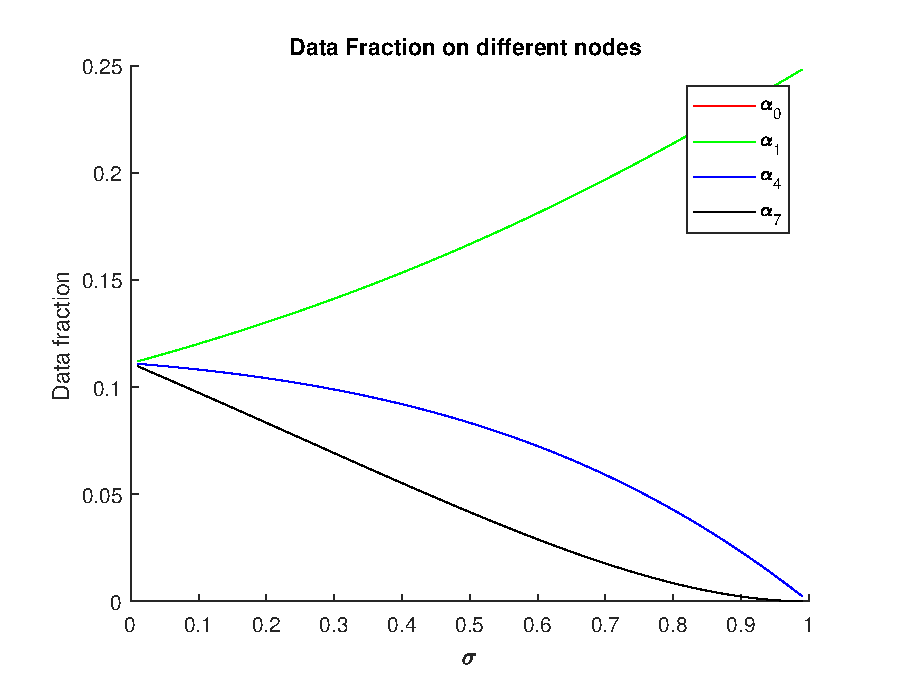
\includegraphics[width=1\columnwidth]{figure/3t3bfraction.eps}
\caption{The data fraction simulation result of 3*3 regular network and the data injection happens on the boundary $P_{0}$}
\label{fig:3t3bfraction}
\end{figure}
$P_{0}$ and $P_{1}$ have the same $\alpha$, so the curve of $\alpha_{0}$ and $\alpha_{1}$ coincide.  
\newpage 
\subsection{Data Injection On The Inner Grid Processor}

\Fig{3t3i} shows that $L$ loads on the inner grid processor $P_{0}$, 
\begin{figure}[!ht]
\centering
\includegraphics[width=0.5\columnwidth]{figure/3t3i.JPG}
\caption{3*3 regular network.  The data injection position is inner grid point $P_{0}$}
\label{fig:3t3i}
\end{figure}
\newpage

The timing diagram for this user case is illustrated as \Fig{3t3id}:
\begin{figure}[!ht]
\centering
\includegraphics[width=0.55\columnwidth]{figure/3t3id.JPG}
\caption{The timing diagram for 3*3 regular network and the data injection is inner grid $P_{0}$}
\label{fig:3t3id}
\end{figure}
\newpage 

The group of equations are:
\begin{empheq}[left=\empheqlbrace]
{align}
\alpha_{0} \omega T_{cp} = T_{f, m}\\
\alpha_{1} \omega T_{cp} = T_{f, m}\\
\alpha_{2} \omega T_{cp} = T_{f, m}\\
\alpha_{3} \omega T_{cp} = T_{f, m}\\
\alpha_{4} \omega T_{cp} = T_{f, m}\\
\alpha_{1}zT_{cm} + \alpha_{5}\omega T_{cp} = T_{f, m}\\
\alpha_{1}zT_{cm} + \alpha_{6}\omega T_{cp} = T_{f, m}\\
\alpha_{1}zT_{cm} + \alpha_{7}\omega T_{cp} = T_{f, m}\\
\alpha_{1}zT_{cm} + \alpha_{8}\omega T_{cp} = T_{f, m}\\
\sigma = \frac{zT_{cm}}{\omega T_{cp}}\\
0 < \sigma < 1 \\
0 < \alpha_{0} \leq 1\\
0 \leq \quad \alpha_{1} \quad \alpha_{2} \quad  \cdots  \quad \alpha_{8} < 1
\end{empheq}
\\

The flow matrix form is :
\begin{equation}
{
\left[ \begin{array}{ccc}
1 & 4 & 4 \\
1 & -1 & 0\\
0 & \sigma-1 & 1\\
\end{array} 
\right ]} \times \left[ \begin{array}{c}
\alpha_{0} \\
\alpha_{1} \\
\alpha_{5} \\
\end{array} 
\right ] = \left[ \begin{array}{c}
1 \\
0 \\
0 
\end{array} 
\right ]
\end{equation}
\newpage 

The simulation result is \Fig{3t3ifraction}:
$P_{0}$ and $P_{1}$ have the same $\alpha$ value, so the curve of $\alpha_{0}$ and $\alpha_{1}$ coincide.  

\begin{figure}[!ht]
\centering
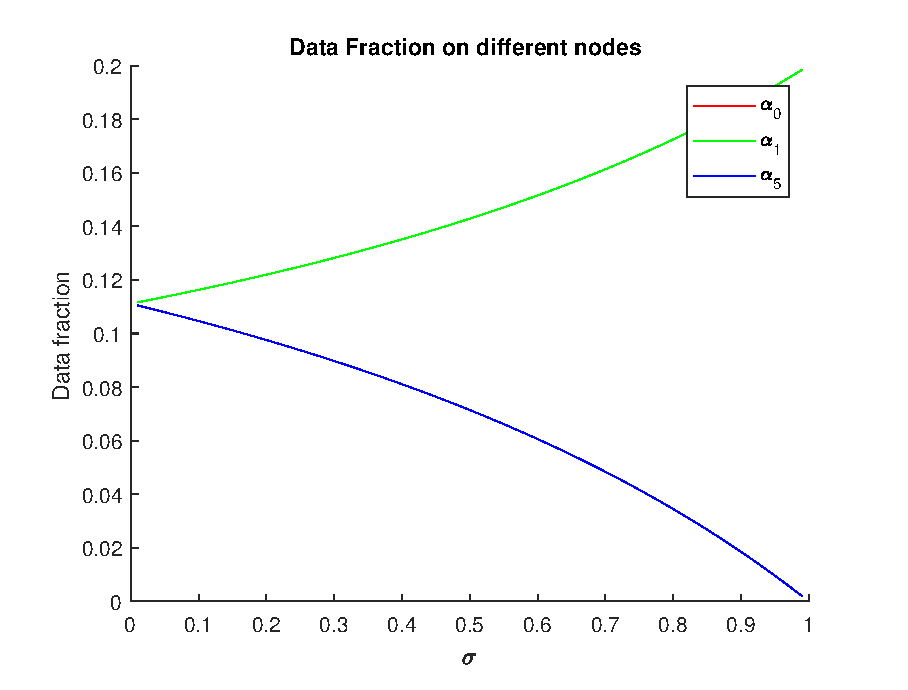
\includegraphics[width=1\columnwidth]{figure/3t3ifraction.eps}
\caption{3*3 regular network.  The data injection position is inner grid point $P_{0}$}
\label{fig:3t3ifraction}
\end{figure}
\subsection{Sensitivity Analysis With Front-end Processors}
From Chapter $2$, we know the speedup is :
$$Speedup = \frac{T_{f, 0}}{T_{f, n}}= \frac{\omega T_{cp}}{\alpha_{0}\omega T_{cp}} = \frac{1}{\alpha_{0}} = \left |-\det A \right |$$.
\subsubsection{Data Injection On The Corner Processor}
The simulation result of sensitivity analysis of $2*n$ regular mesh \Fig{2t10} is as follows:
\begin{figure}[!ht]
\centering
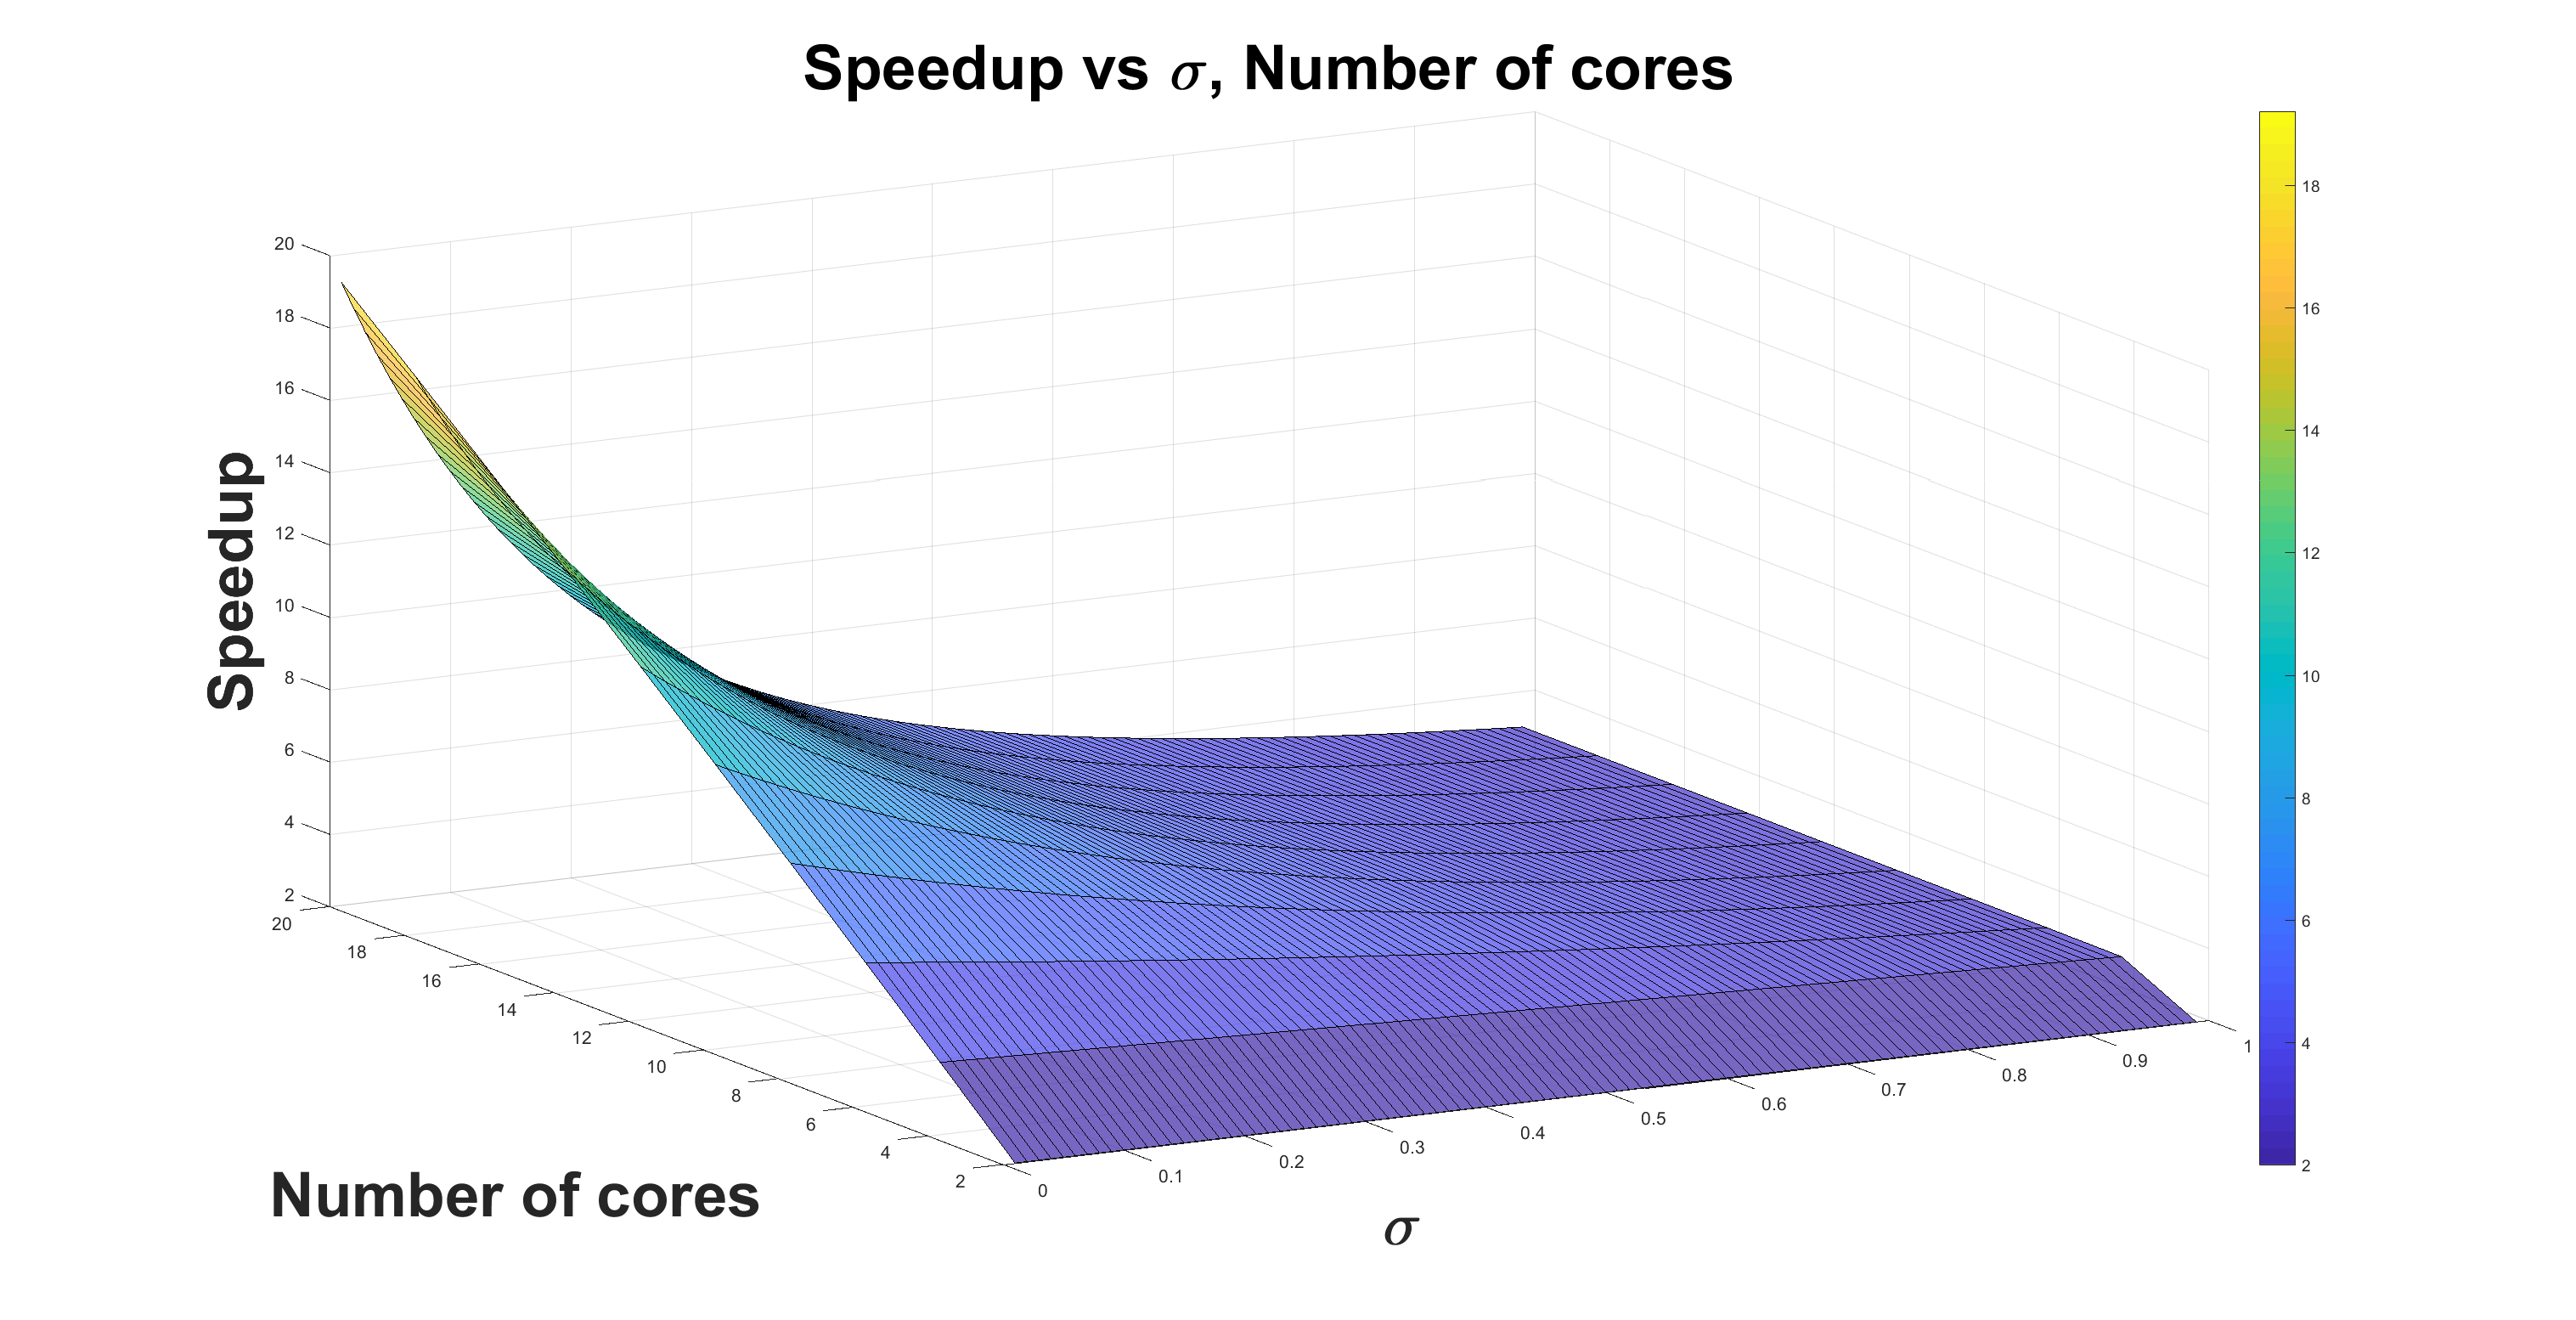
\includegraphics[width=1\columnwidth]{figure/sa2t10c.eps}
\caption{Sensitivity analysis result of 2*10 regular mesh result}
\label{fig:sa2t10c}
\end{figure}

\newpage
\subsubsection{Data Injection On The Boundary Processor}
Talking to \Fig{3t8}, the data injection happens on boundary processor $P_{2}$. 
\begin{figure}[!ht]
\centering
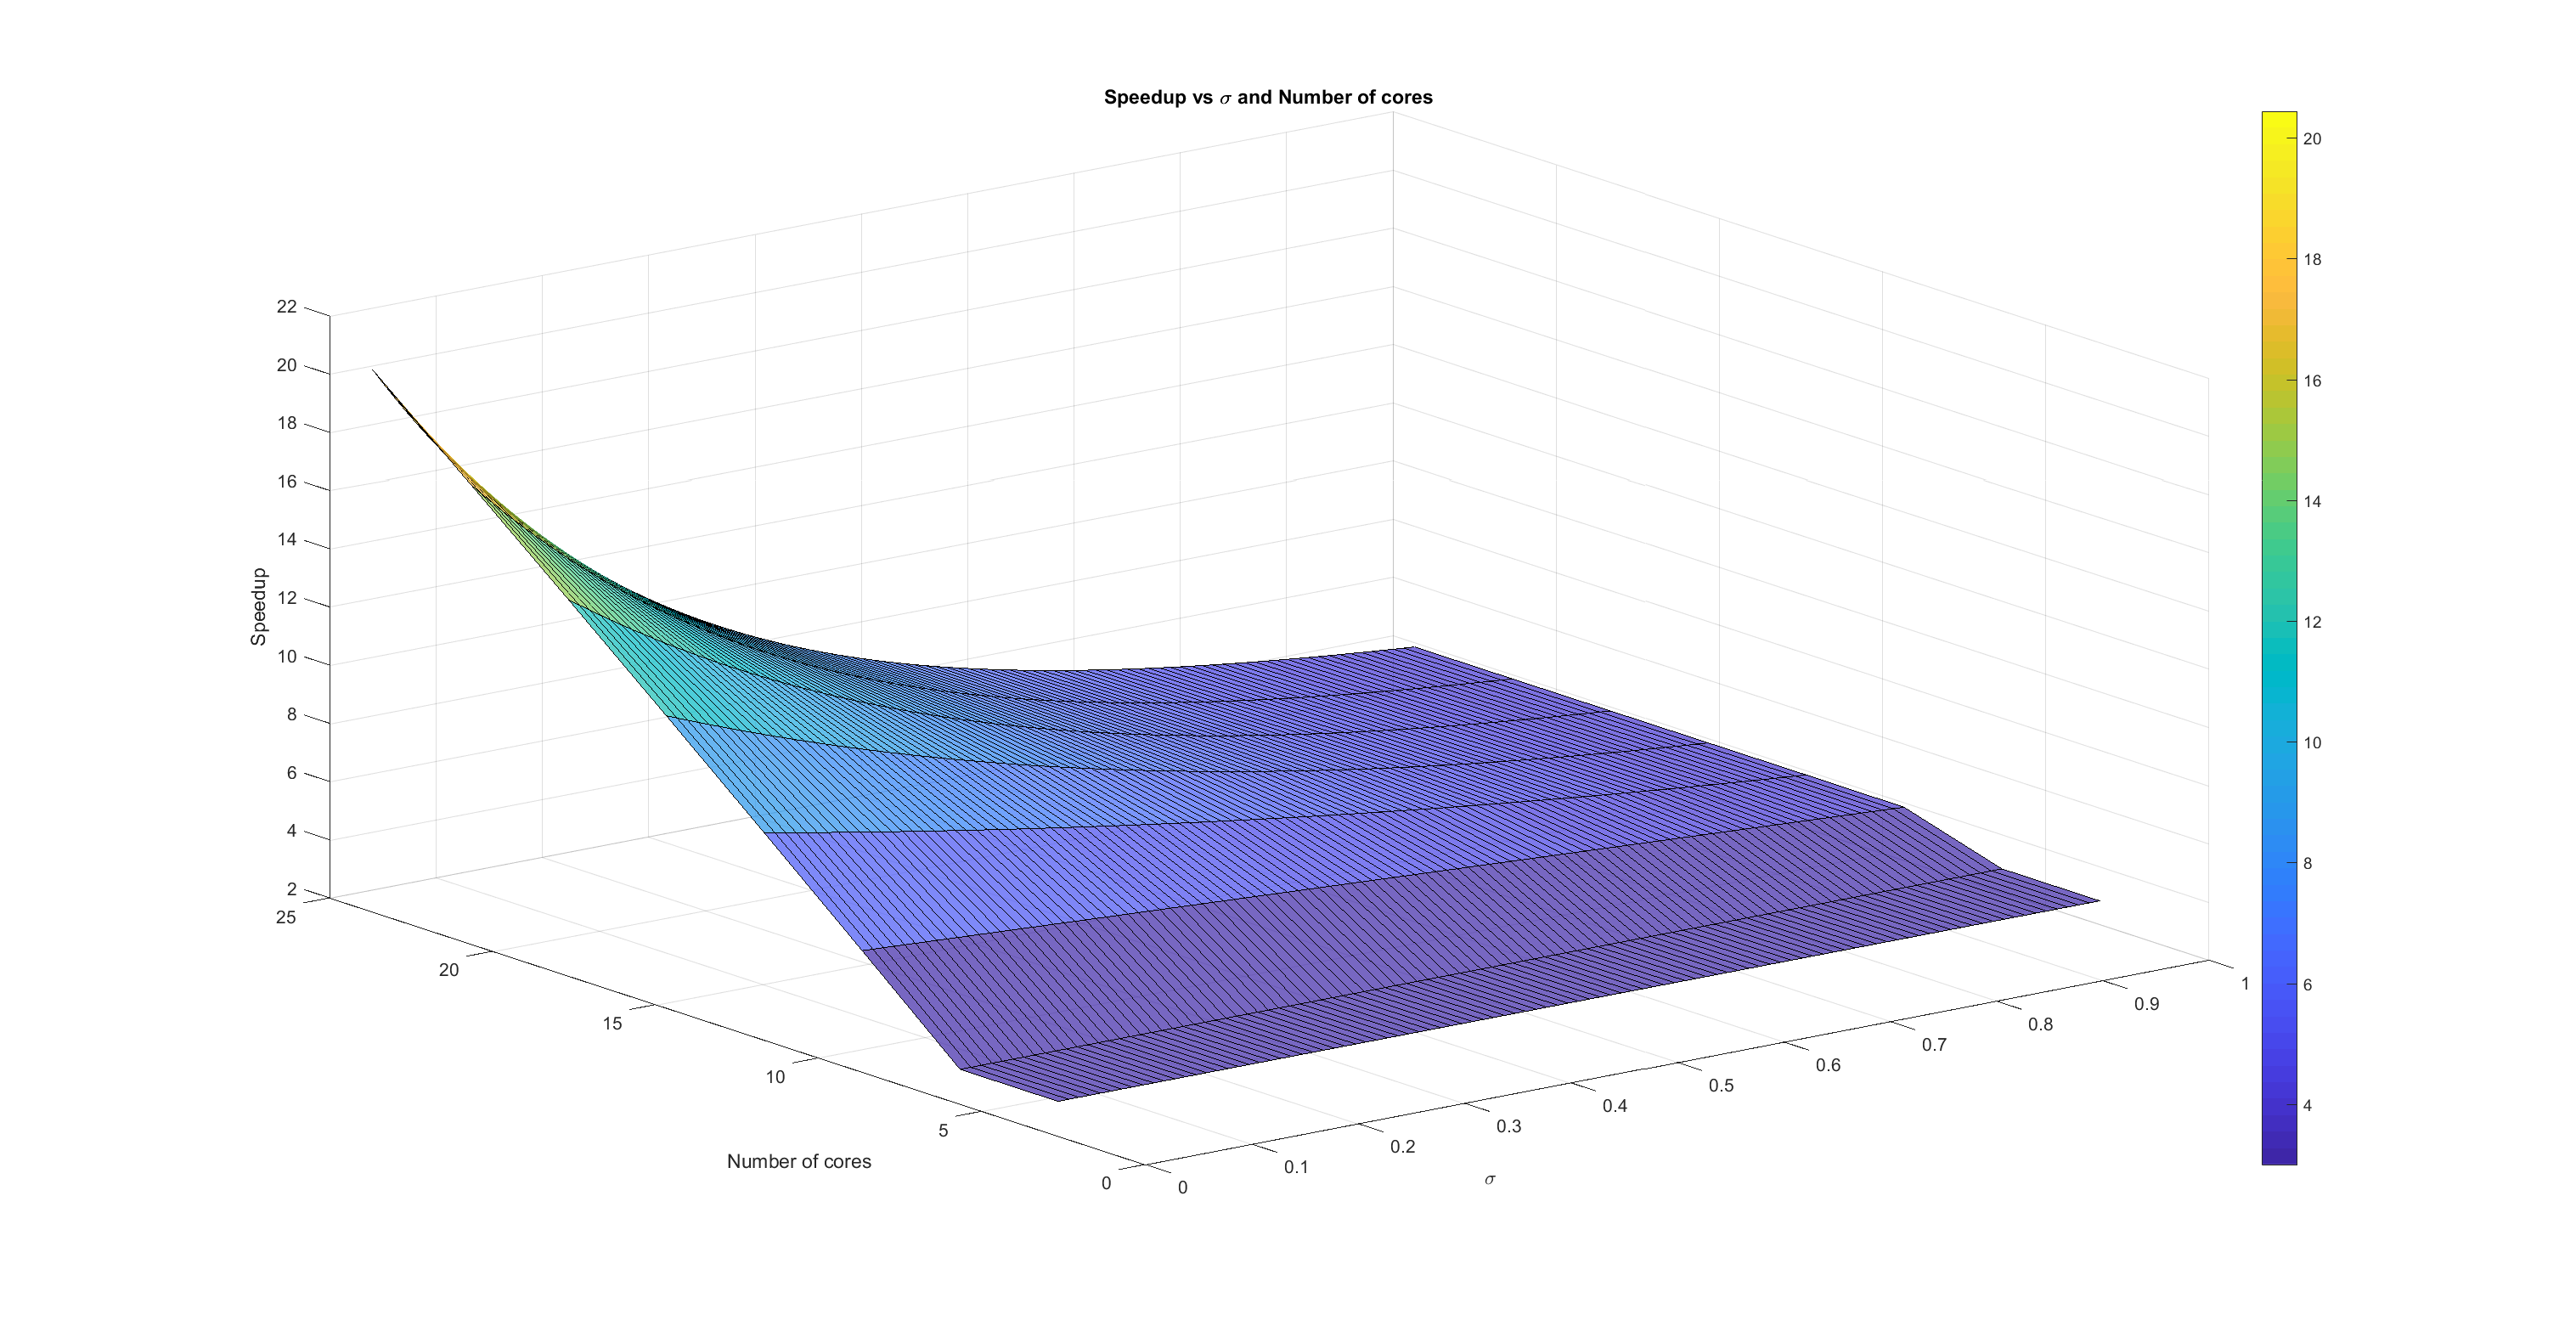
\includegraphics[width=1\columnwidth]{figure/sa3t8b.eps}
\caption{Sensitivity analysis result of 3*8 regular network and the injection position on boundary processor $P_{2}$}
\label{fig:sa3t8b}
\end{figure}
\Fig{sa3t8b} shows that if the value $\sigma > 0.2$, the speedup simulation effect is obvious.   If the value $\sigma < 0.1$, the number of cores has linear impact on the speedup performance.   If the number of cores $>$ 5, the bottom effect with front-end, the cluster at least get about $4$ times speedup.   The reason is $P_{0}$ has $3$ $level_{1}$ processors.  

\newpage

\subsubsection{Data Injection On The Inner Grid Processor}
\Fig{5t5}, $L$ incurs on $P_{12}$ and the simulation result says:
\begin{figure}[!ht]
\centering
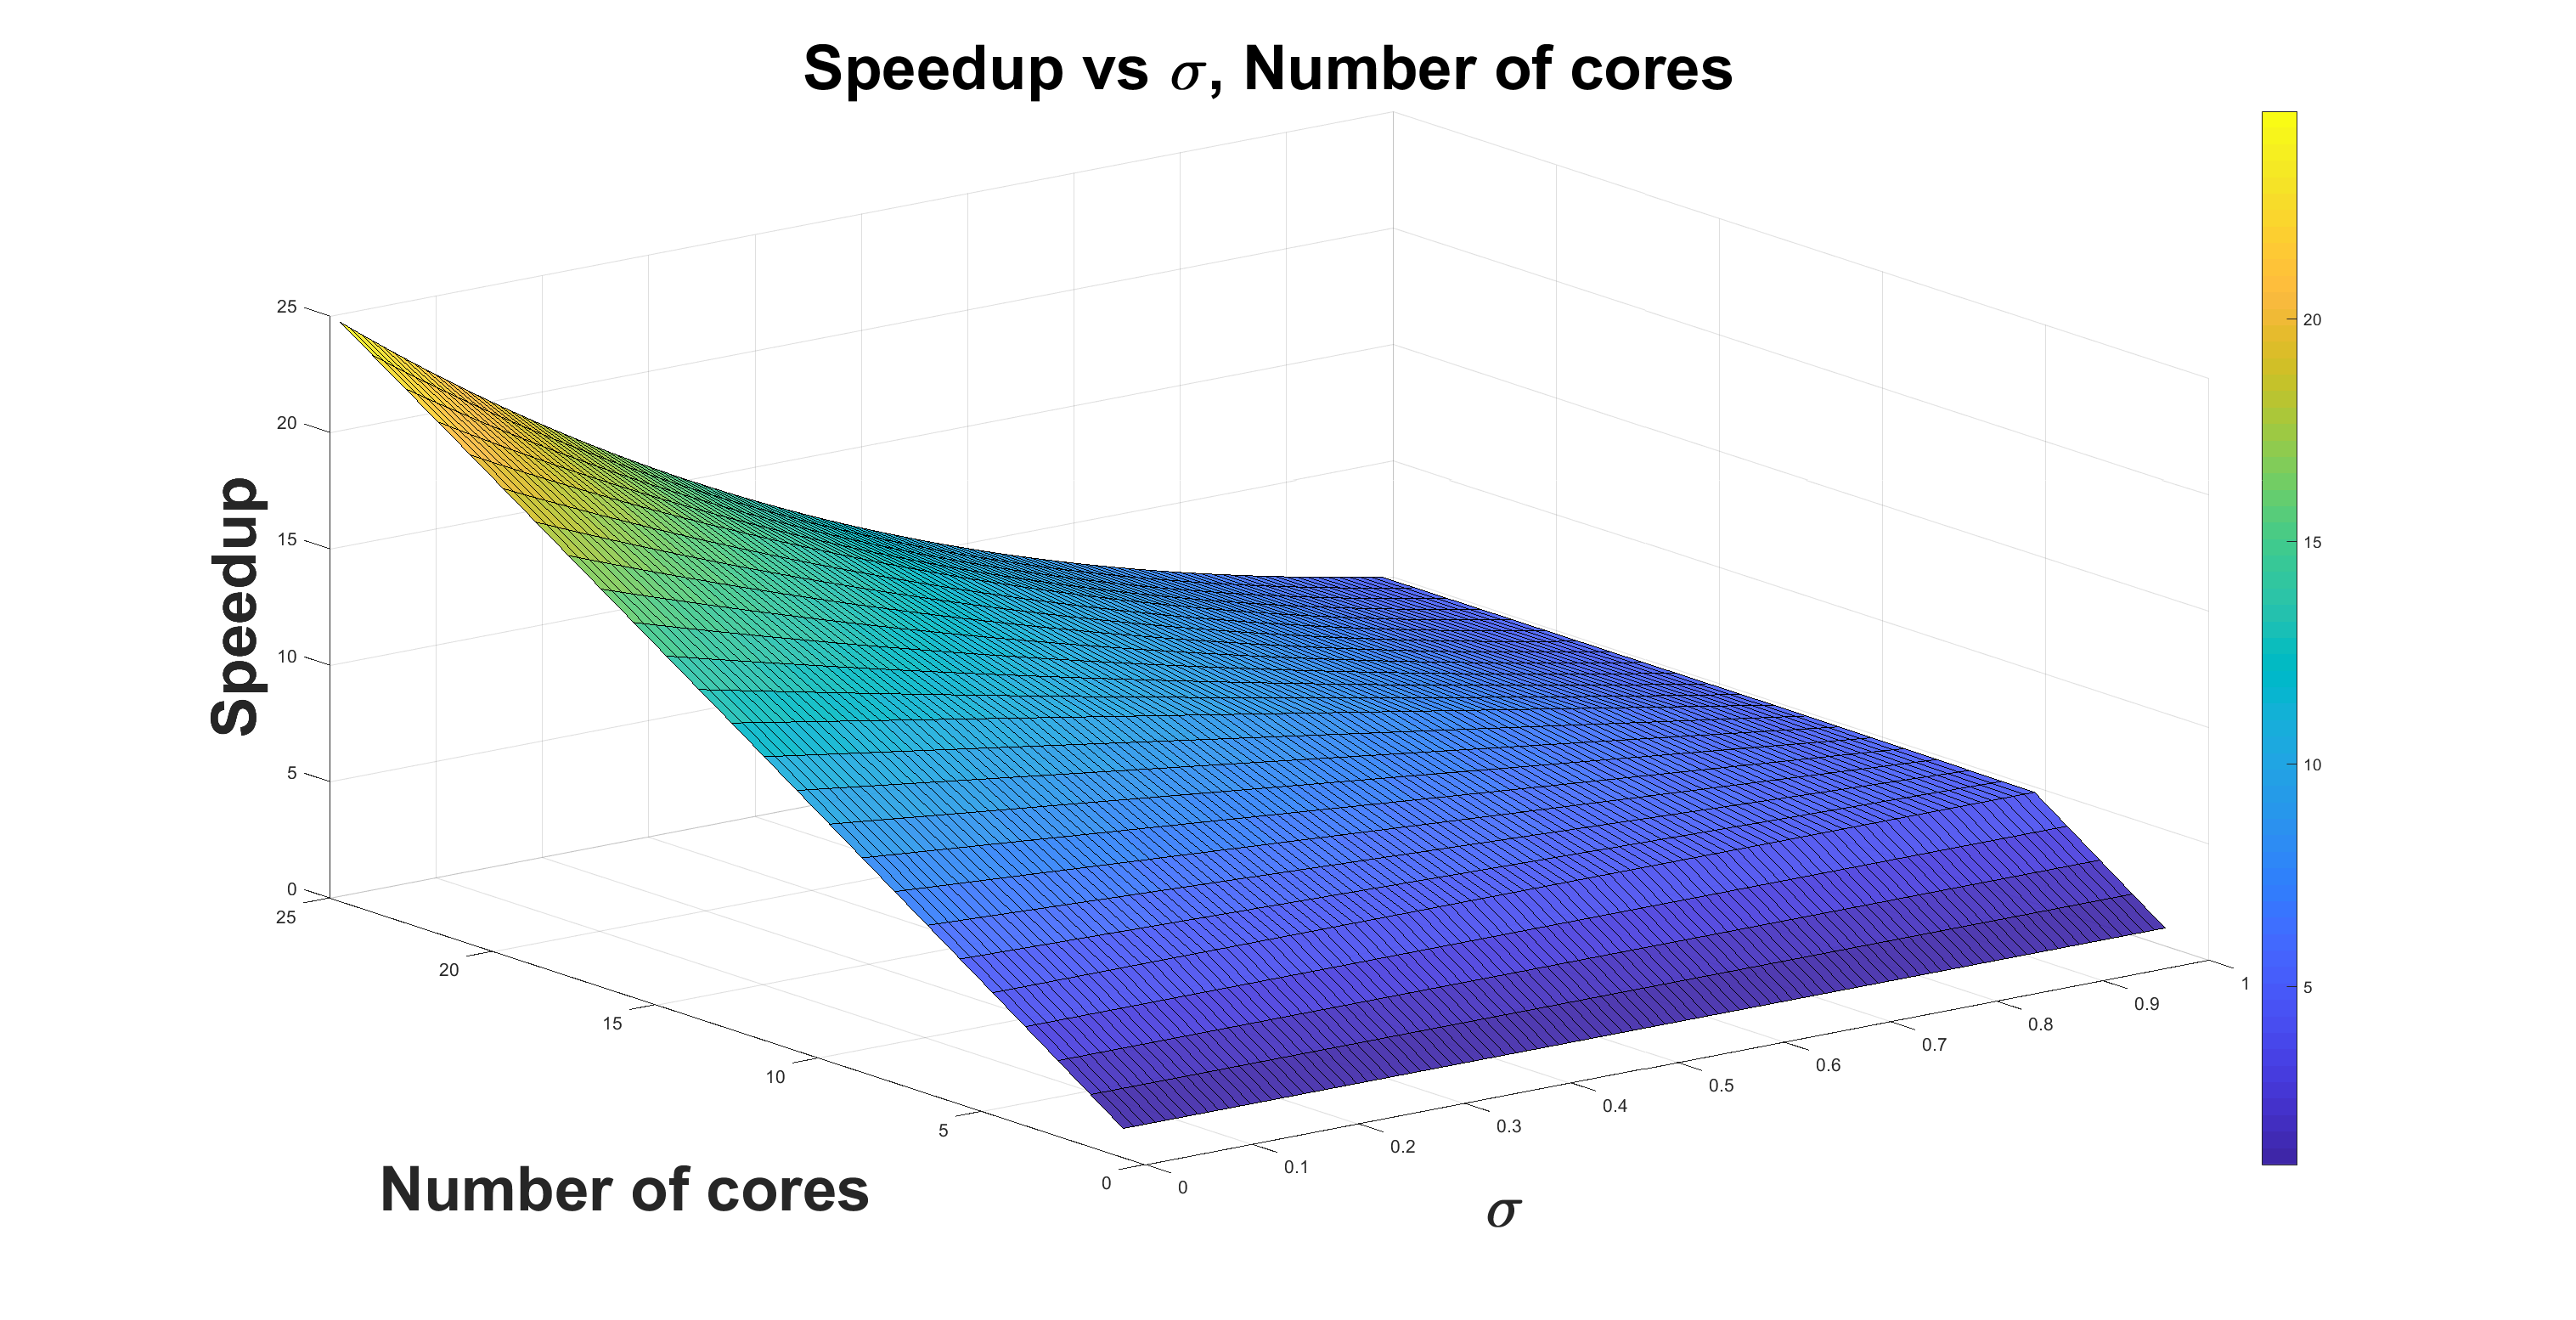
\includegraphics[width=1\columnwidth]{figure/sa5t5i.eps}
\caption{Sensitivity analysis result of data injection position on inner grid processor}
\label{fig:sa5t5i}
\end{figure}
If the number of processor large than $5$, the cluster equivalence computation ability is at least $5$ time speedup.  It is the inner grid has $4$ $level_{1}$ neighbor processors.  
\newpage

\input{RegularMesh_Multi_even.tex}
\input{RegularMesh_Multi_no_even.tex}
\section{Without Front-end Scenario}

In the without front-end scenario, the processors solely start to process as soon as each processor receives its entire load assignment\cite{gamboa2011simple}.  

This subsection concerns the processors without front-end.  Because of without front-end, the processors simultaneously receive the data and solely start to process it as soon as each processor receives its entire load assignment.  \\
We consider the timing diagram for \Fig{2t2}, \Fig{2t3}, \Fig{2t10} and so on.   In addition, we also give the new closed-form matrix equations for the previous user cases.  \\
The rule also plays a dominate role in establish the mathematics model.  \\
\subsection{Data Injection on The Corner Processor}
\subsubsection{2*2 Regular Network}
The timing diagram of \Fig{2t2} is shown:

\begin{figure}[!ht]
\centering
\includegraphics[width=0.5\columnwidth]{figure/2t2d_no.JPG}
\caption{The timing diagram for 2*2 regular network without front-end.  }
\label{fig:2t2d_no}
\end{figure}
\newpage 

$P_{0}$ starts to process the assigned workload and it starts to transfer the $\alpha_{1}$, $\alpha_{2}$  and $\alpha_{3}$ fraction workload after it totally receive its $\alpha_{0}$ task.  That is,  $P_{1}$ and $P_{2}$ are idle until the $L$ finish its data injection to $P_{0}.  $The similar situation happens to $P_{1}$ and $P_{2}$ and they both start to transmit the $\alpha_{3}$ after they totally receive the appropriate workload.  In other words, $P_{3}$ has to wait until the previous two layer processors obtain their own data. 

The corresponding group of equations are as follows:

\begin{empheq}[left=\empheqlbrace]
{align}
\alpha_{0} \omega T_{cp} = T_{f, m}\\
\alpha_{1}zT_{cm} + \alpha_{1} \omega T_{cp} = T_{f, m}\\
\alpha_{2}zT_{cm} + \alpha_{2} \omega T_{cp} = T_{f, m}\\
(\alpha_{1} + \alpha_{3})zT_{cm} + \alpha_{3}\omega T_{cp} = T_{f, m}\\
\sigma = \frac{zT_{cm}}{\omega T_{cp}}\\
\alpha_{0} + \alpha_{1} +\alpha_{2} + \alpha_{3} = 1\\
0 < \sigma < 1 \\
0 < \alpha_{0} \leq 1\\
0 \leq \alpha_{1},  \alpha_{2},  \alpha_{3}  < 1
\end{empheq}
\\
The matrix closed-from is presented as:
\begin{equation}
{
\left[ \begin{array}{ccc}
1 & 2 & 1\\
1 & -(\sigma + 1) & 0\\
1 & -\sigma & -(\sigma + 1)
\end{array} 
\right ]} \times \left[ \begin{array}{c}
\alpha_{0} \\
\alpha_{1} \\
\alpha_{3} 
\end{array} 
\right ] = \left[ \begin{array}{c}
1 \\
0 \\
0 
\end{array} 
\right ]
\end{equation}
\\
The explicit solution is:
\begin{empheq}[left=\empheqlbrace]
{align}
\alpha_{0} = (\frac{\sigma + 1}{\sigma + 2})^{2}\\
\alpha_{1} = \frac{\sigma + 1}{(\sigma + 2)^{2}}\\
\alpha_{3} = \frac{1}{(\sigma + 2)^{2}}
\end{empheq}
\\
The simulation result for \Fig{2t2} is provided in \Fig{2t2_no_fraction}:
\begin{figure}[!ht]
\centering
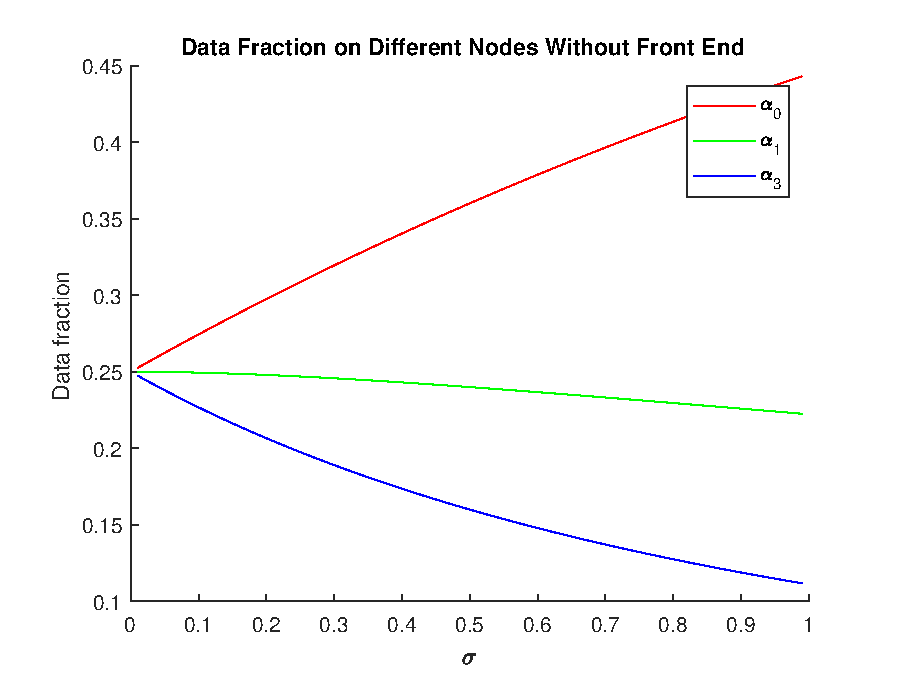
\includegraphics[width=1\columnwidth]{figure/2t2_no_fraction.eps}
\caption{The data fraction deployed based on the radius value }
\label{fig:2t2_no_fraction}
\end{figure}
\newpage

\Fig{2t2_no_fraction} explains that as the value $\sigma$ grows up,  as the fraction assigned to $P_{0}$ increases, the fractions distributed to $level_{1}$ and $level_{2}$ reduces.  In other words, if the communication capability decreases, there are more data processed locally, which is reasonable.  If the ability of the link degrades, asymptotically equaling to the processor computation capacity, there is solely $11\%$ data is deployed to the $level_{2}$.  In addition, if the $\sigma > 1$,  it means that the transmitting power is less than the processor's processing ability.  In this scenario, keeping the data locally is more economical than transmitting it.  
\newpage

\subsubsection*{2*3 Regular Network}

$P_{0}$ starts to process the assigned workload and it starts to transfer the $\alpha_{1}$, $\alpha_{2}$, $\alpha_{3}$, $\alpha_{4}$, $\alpha_{5}$ fraction workload after it totally receive its $\alpha_{0}$ task.  That is,  $P_{1}$ and $P_{2}$ are idle until the $L$ finishes its data injection to $P_{0}$.  According to the $level_{1}$, the similar situation happens to $P_{1}$ and $P_{2}$ and they both start to transmit the $\alpha_{3}$ after they totally receive the appropriate workload.  In other words, $P_{3}$ has to wait until the previous three layers,  $level_{0}$,  $level_{1}$ and $level_{2}$ processors obtain their own data.  

\begin{figure}[!ht]
\centering
\includegraphics[width=0.65\columnwidth]{figure/2t3d_no.JPG}
\caption{The timing diagram for 2*3 regular network without front-end.  }
\label{fig:2t3d_no}
\end{figure}

In addition,  the group of equations are as follows:
\begin{empheq}[left=\empheqlbrace]
{align}
\alpha_{0} \omega T_{cp} = T_{f, m}\\
\alpha_{1}zT_{cm} + \alpha_{1} \omega T_{cp} = T_{f, m}\\
\alpha_{2}zT_{cm} + \alpha_{2} \omega T_{cp} = T_{f, m}\\
(\alpha_{1} + \alpha_{3})zT_{cm} + \alpha_{3}\omega T_{cp} = T_{f, m}\\
(\alpha_{1} + \alpha_{4})zT_{cm} + \alpha_{4}\omega T_{cp} = T_{f, m}\\
(\alpha_{1} + \alpha_{3} + \alpha_{5})zT_{cm} + \alpha_{5}\omega T_{cp} = T_{f, m}\\
\sigma = \frac{zT_{cm}}{\omega T_{cp}}\\
\alpha_{0} + \alpha_{1} +\alpha_{2} + \alpha_{3} + \alpha_{4} + \alpha_{5} = 1\\
0 < \alpha_{0} \leq 1\\
0 \leq \alpha_{1} \quad \alpha_{2} \quad \alpha_{3} \quad \alpha_{4} \quad \alpha_{5} < 1
\end{empheq}

The flow matrix is :
\begin{equation}
{
\left[ \begin{array}{cccc}
1 & 2 & 2 & 1\\
1 & -(\sigma + 1) & 0 & 0\\
1 & -\sigma & -(\sigma + 1) & 0\\
1 & -\sigma & -\sigma & -(\sigma + 1)
\end{array} 
\right ]} \times \left[ \begin{array}{c}
\alpha_{0} \\
\alpha_{1} \\
\alpha_{3} \\
\alpha_{5}
\end{array} 
\right ] = \left[ \begin{array}{c}
1 \\
0 \\
0 \\
0
\end{array} 
\right ]
\end{equation}
\\
The speedup is 
$$Speedup = \frac{T_{f, 0}}{T_{f, n}}= \frac{\omega T_{cp}}{\alpha_{0}\omega T_{cp}} = \frac{1}{\alpha_{0}}$$

The explicit solution is:
\begin{empheq}[left=\empheqlbrace]
{align}
\alpha_{0} = (\frac{\sigma + 1}{\sigma + 2})^{3}\\
\alpha_{1} = \frac{(\sigma + 1)^{2}}{(\sigma + 2)^{3}}\\
\alpha_{3} = \frac{\sigma + 1}{(\sigma + 2)^{3}}\\
\alpha_{5} = \frac{1}{(\sigma + 2)^{3}}
\end{empheq}
\\
The simulation result is:

\begin{figure}[!ht]
\centering
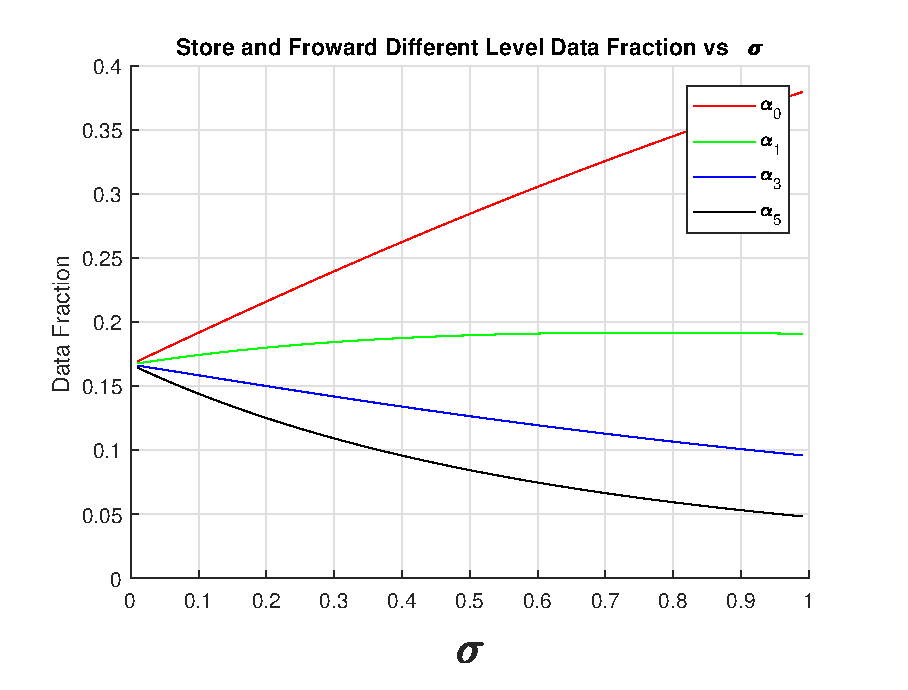
\includegraphics[width=1\columnwidth]{figure/2t3_no_fraction.eps}
\caption{The data fraction deployed based on the radius value }
\label{fig:2t3_no_fraction}
\end{figure}
\newpage

\subsubsection{2*n Regular Network}

Considering \Fig{2t10}, the equations are demonstrated as follows:

\begin{empheq}[left=\empheqlbrace]
{align}
\alpha_{0} \omega T_{cp} = T_{f, m}\\
\alpha_{1}zT_{cm} + \alpha_{1} \omega T_{cp} = T_{f, m}\\
\alpha_{2}zT_{cm} + \alpha_{2} \omega T_{cp} = T_{f, m}\\
(\alpha_{1} + \alpha_{3})zT_{cm} + \alpha_{3}\omega T_{cp} = T_{f, m}\\
(\alpha_{1} + \alpha_{4})zT_{cm} + \alpha_{4}\omega T_{cp} = T_{f, m}\\
(\alpha_{1} + \alpha_{3} + \alpha_{5})zT_{cm} + \alpha_{5}\omega T_{cp} = T_{f, m}\\
\vdots\\
(\alpha_{1} + \alpha_{3} +\cdots + \alpha_{2 \times n - 1})zT_{cm} +\alpha_{2 \times n - 1} \omega T_{cp} = T_{f, m}\\
\sigma = \frac{zT_{cm}}{\omega T_{cp}}\\
0 < \sigma < 1 \\
0 < \alpha_{0} \leq 1\\
0 \leq \quad \alpha_{1} \quad \alpha_{3} \quad  \cdots  \quad \alpha_{2 \times n - 1} < 1
\end{empheq}

Use $\sigma^{\star}$ to present $-(\sigma + 1)$ and the flow matrix form for the group of equations is :

\begin{equation}
{
\left[ \begin{array}{ccccccc}
1 & 2 & 2 & \cdots & 2 & 2 & 1\\
1 & \sigma^{\star} & 0 & \cdots& 0 & 0 & 0\\
1 & -\sigma & \sigma^{\star} & \cdots & 0 & 0 & 0 \\
1 & -\sigma & -\sigma & \sigma^{\star} & 0 & \cdots & 0 \\
1 & -\sigma & -\sigma & -\sigma & \sigma^{\star} & 0 & 0 \\
\vdots & \vdots & \vdots  &   \vdots & \ddots & \ddots\\
1 & -\sigma & -\sigma & \cdots & -\sigma & -\sigma & \sigma^{\star}
\end{array} 
\right ]} \times \left[ \begin{array}{c}
\alpha_{0} \\
\alpha_{1} \\
\alpha_{3} \\
\alpha_{5} \\
\vdots \\
\alpha_{2 \times n - 3}\\
\alpha_{2 \times n - 1}
\end{array} 
\right ] = \left[ \begin{array}{c}
1 \\
0 \\
0 \\
0 \\
\vdots \\
0
\end{array} 
\right ]
\end{equation}

According to the \textbf{\textit{Cramer's rule}},the explicit solution for the group of equations is:
\begin{empheq}[left=\empheqlbrace]
{align}
\alpha_{i} = \left |\frac{\det A^{\star}_{i}}{\det A}\right |
\end{empheq}
where $A^{\star}_{i}$ is the matrix formed by replacing the $i$-th column of A by the column vector b.
\newpage

We use  $-\sigma - 2 = \epsilon$ and $\sigma^{\star} -2 = \beta$.  After a series of column reduction and row reduction, the flow matrix changes as follows :
\begin{equation*}
     {A = \left[ \begin{array}{ccccccc}
1 & 2 & 2 & \cdots & 2 & 2 & 1\\
1 & {\sigma}^{\star} & 0 & 0 & 0 & 0 &0\\
1 & -\sigma & {\sigma}^{\star} & 0 & 0 & 0 & 0 \\
1 & -\sigma & -\sigma & {\sigma}^{\star} & 0 & 0 & 0 \\
1 & -\sigma & -\sigma & -\sigma & {\sigma}^{\star} & 0 & 0\\
1 & -\sigma & -\sigma & -\sigma & -\sigma & {\sigma}^{\star} & 0\\
1 & -\sigma & -\sigma & -\sigma & -\sigma & -\sigma & {\sigma}^{\star}\\
\end{array} 
\right ]
\xrightarrow[\text{Reduction}]{\text{Column}}\\
\left[ \begin{array}{ccccccc}
1 & 0 & 0 & \cdots & 0 & 0 & 0\\
1 & \beta & -2 & \cdots& -2 & -2 & -1\\
1 & \epsilon & \beta & \cdots & 0 & 0 & 0 \\
1 & \epsilon & \epsilon & \beta & 0 & \cdots & 0 \\
1 & \epsilon & \epsilon & \epsilon & \beta & 0 & 0 \\
\vdots & \vdots & \vdots  &   \vdots & \ddots & \ddots\\
1 & \epsilon & \epsilon & \cdots & \epsilon & \epsilon & \beta
\end{array} 
\right ]
}
\end{equation*}

\begin{equation*}
{\xrightarrow[\text{Reduction}]{\text{Row}}\\
\left[ \begin{array}{ccccccc}
1 & 0 & 0 & \cdots & 0 & 0 & 0\\
0 & \beta & -2 & \cdots& -2 & -2 & -1\\
0 & \epsilon & \beta & \cdots & 0 & 0 & 0 \\
0 & \epsilon & \epsilon & \beta & 0 & \cdots & 0 \\
0 & \epsilon & \epsilon & \epsilon & \beta & 0 & 0 \\
\vdots & \vdots & \vdots  &   \vdots & \ddots & \ddots\\
0 & \epsilon & \epsilon & \cdots & \epsilon & \epsilon & \beta
\end{array} 
\right ]
}
\end{equation*}

We define
\begin{equation*}
{C = \left[ \begin{array}{cccccc}
{\sigma}^{\star} & 0 & 0 & 0 & 0 &0\\
-\sigma & {\sigma}^{\star} & 0 & 0 & 0 & 0 \\
-\sigma & -\sigma & {\sigma}^{\star} & 0 & 0 & 0 \\
-\sigma & -\sigma & -\sigma & {\sigma}^{\star} & 0 & 0\\
-\sigma & -\sigma & -\sigma & -\sigma & {\sigma}^{\star} & 0\\
-\sigma & -\sigma & -\sigma & -\sigma & -\sigma & {\sigma}^{\star}\\
\end{array} 
\right ]
}
\end{equation*}

$0 < \sigma < 1$, then $-2 < \sigma^{\star} < -1$, which means $C$ is column linear independent, after column and row reduction. \\
Further, we define
\begin{equation*}
{\hat{C} = \left[ \begin{array}{cccccc}
\beta & -2 & \cdots& -2 & -2 & -1\\
\epsilon & \beta & \cdots & 0 & 0 & 0 \\
\epsilon & \epsilon & \beta & 0 & \cdots & 0 \\
\epsilon & \epsilon & \epsilon & \beta & 0 & 0 \\
\vdots & \vdots & \vdots  &   \vdots & \ddots & \ddots\\
\epsilon & \epsilon & \cdots & \epsilon & \epsilon & \beta
\end{array} 
\right ]
}
\end{equation*}

$C^{\star}$ is full rank.\\
So the flow matrix $A$ is full rank, that is, $\det A \neq 0$ and $\det A^{*} \neq 0$.
The speedup is  
$$Speedup = \frac{T_{f, 0}}{T_{f, n}}= \frac{\omega T_{cp}}{\alpha_{0}\omega T_{cp}} = \frac{1}{\alpha_{0}} = \frac{\det A}{\det A^{\star}} = \left |\frac{\det A}{(\sigma^{\star})^{n-1}}\right|$$
\newpage 

\subsubsection{m*n Regular Network}
Referring to \Fig{5t5}, we utilize ${\sigma}^{\star}$ to present the $-(\sigma + 1)$.  The matrix closed-form is:
\begin{equation}
{
\left[ \begin{array}{ccccccccc}
1 & 2 & 3 & 4 & 5 & 4 & 3 & 2 & 1\\
1 & {\sigma}^{\star} & 0 & 0 & 0 & 0 & 0 & 0 & 0\\
1 & -\sigma & {\sigma}^{\star} & 0 & 0 & 0 & 0& 0 & 0 \\
1 & -\sigma & -\sigma & {\sigma}^{\star} & 0 &0 & 0 & 0 & 0 \\
1 & -\sigma & -\sigma & -\sigma & {\sigma}^{\star} & 0 & 0 & 0 & 0\\
1 & -\sigma & -\sigma & -\sigma & -\sigma & {\sigma}^{\star} & 0 & 0 & 0\\
1 & -\sigma & -\sigma & -\sigma & -\sigma & -\sigma & {\sigma}^{\star} & 0 & 0\\
1 & -\sigma & -\sigma & -\sigma & -\sigma & -\sigma & -\sigma & {\sigma}^{\star} &0\\
1 & -\sigma & -\sigma & -\sigma & -\sigma & -\sigma & -\sigma & -\sigma & {\sigma}^{\star}\\
\end{array} 
\right ]} \times \left[ \begin{array}{c}
\alpha_{0} \\
\alpha_{1} \\
\alpha_{3} \\
\alpha_{6} \\
\alpha_{10} \\
\alpha_{15}\\
\alpha_{19}\\
\alpha_{22}\\
\alpha_{24}
\end{array} 
\right ] = \left[ \begin{array}{c}
1 \\
0 \\
0 \\
0 \\
0\\
0\\
0\\
0\\
0
\end{array} 
\right ]
\end{equation}
\newpage

\subsection{Data Injection on The Boundary Processor}
\Fig{3t3b} shows an example of boundary processor $P_{0}$ receiving $L$.
The timing diagram for \Fig{3t3b} is \Fig{3t3bd_no}.  

\begin{figure}[!ht]
\centering
\includegraphics[width=0.5\columnwidth]{figure/3t3bd_no.JPG}
\caption{The timing diagram for 3*3 boundary data injection on $P_{0}$ }
\label{fig:3t3bd_no}
\end{figure}
The equations are:
\begin{empheq}[left=\empheqlbrace]
{align}
\alpha_{0} \omega T_{cp} = T_{f, m}\\
\alpha_{1}zT_{cm} + \alpha_{1} \omega T_{cp} = T_{f, m}\\
\alpha_{2}zT_{cm} + \alpha_{2} \omega T_{cp} = T_{f, m}\\
\alpha_{3}zT_{cm} + \alpha_{3} \omega T_{cp} = T_{f, m}\\
(\alpha_{1} + \alpha_{4})zT_{cm} + \alpha_{4}\omega T_{cp} = T_{f, m}\\
(\alpha_{2} + \alpha_{5})zT_{cm} + \alpha_{5}\omega T_{cp} = T_{f, m}\\
(\alpha_{3} + \alpha_{6})zT_{cm} + \alpha_{6}\omega T_{cp} = T_{f, m}\\
(\alpha_{1} + \alpha_{4} +\alpha_{7})zT_{cm} + \alpha_{7}\omega T_{cp} = T_{f, m}\\
(\alpha_{1} + \alpha_{4} +\alpha_{8})zT_{cm} + \alpha_{8}\omega T_{cp} = T_{f, m}\\
\sigma = \frac{zT_{cm}}{\omega T_{cp}}\\
0 < \sigma < 1 \\
0 < \alpha_{0} \leq 1\\
0 \leq \quad \alpha_{1} \quad \alpha_{3} \quad \alpha_{4} \quad \alpha_{5} \quad \alpha_{6} \quad \alpha_{7} \quad \alpha_{8}  < 1
\end{empheq}
The flow matrix is :
\begin{equation}
{
\left[ \begin{array}{cccc}
1 & 3 & 3 & 2\\
1 & -(\sigma + 1) & 0 & 0\\
1 & -\sigma & -(\sigma + 1) & 0\\
1 & -\sigma & -\sigma & -(\sigma + 1)
\end{array} 
\right ]} \times \left[ \begin{array}{c}
\alpha_{0} \\
\alpha_{1} \\
\alpha_{4} \\
\alpha_{7}
\end{array} 
\right ] = \left[ \begin{array}{c}
1 \\
0 \\
0 \\
0
\end{array} 
\right ]
\end{equation}
\newpage 
The simulation result is shown in :
\begin{figure}[!ht]
\centering
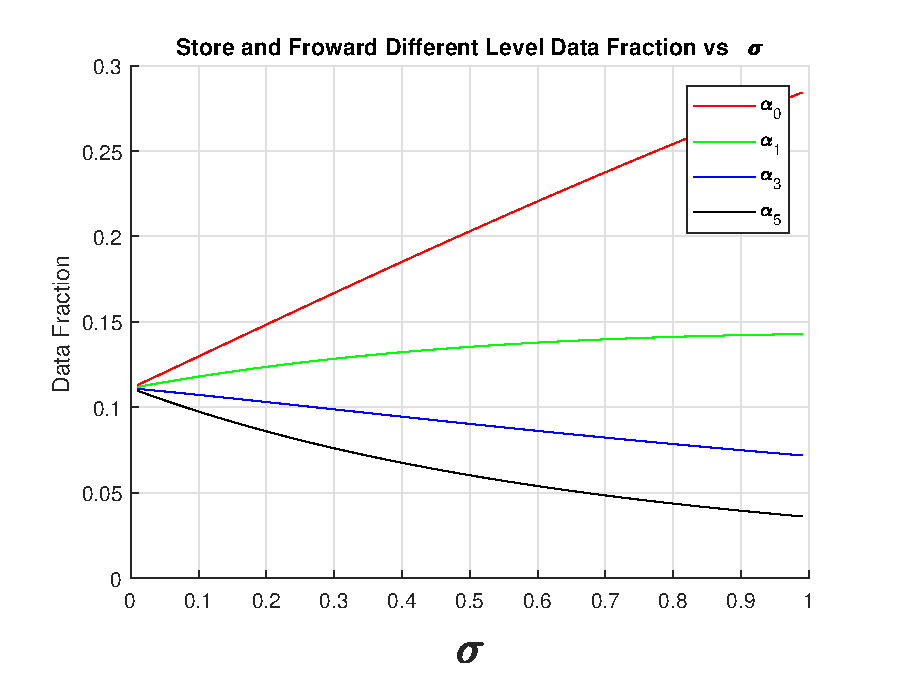
\includegraphics[width=1\columnwidth]{figure/3t3b_no_fraction.eps}
\caption{The fraction curve for 3*3 boundary data injection on $P_{0}$ }
\label{fig:3t3b_no_fraction}
\end{figure}

\newpage

\subsection{Data Injection on The Inner Grid Processor}
The equations are:
\begin{empheq}[left=\empheqlbrace]
{align}
\alpha_{0} \omega T_{cp} = T_{f, m}\\
\alpha_{1}zT_{cm} + \alpha_{1} \omega T_{cp} = T_{f, m}\\
\alpha_{2}zT_{cm} + \alpha_{2} \omega T_{cp} = T_{f, m}\\
\alpha_{3}zT_{cm} + \alpha_{3} \omega T_{cp} = T_{f, m}\\
\alpha_{4}zT_{cm} + \alpha_{4} \omega T_{cp} = T_{f, m}\\
(\alpha_{1} + \alpha_{5})zT_{cm} + \alpha_{5}\omega T_{cp} = T_{f, m}\\
(\alpha_{2} + \alpha_{6})zT_{cm} + \alpha_{6}\omega T_{cp} = T_{f, m}\\
(\alpha_{3} + \alpha_{7})zT_{cm} + \alpha_{7}\omega T_{cp} = T_{f, m}\\
(\alpha_{4} + \alpha_{8})zT_{cm} + \alpha_{8}\omega T_{cp} = T_{f, m}\\
\sigma = \frac{zT_{cm}}{\omega T_{cp}}\\
0 < \sigma < 1 \\
0 < \alpha_{0} \leq 1\\
0 \leq \quad \alpha_{1} \quad \alpha_{3} \quad \alpha_{4} \quad \alpha_{5} \quad \alpha_{6} \quad \alpha_{7} \quad \alpha_{8}  < 1
\end{empheq}
The flow matrix closed-form is:
\begin{equation}
{
\left[ \begin{array}{ccc}
1 & 4 & 4 \\
1 & -(\sigma + 1) & 0\\
1 & -\sigma & -(\sigma + 1)\\
\end{array} 
\right ]} \times \left[ \begin{array}{c}
\alpha_{0} \\
\alpha_{1} \\
\alpha_{5} \\
\end{array} 
\right ] = \left[ \begin{array}{c}
1 \\
0 \\
0 
\end{array} 
\right ]
\end{equation}

The simulation result shows:
\begin{figure}[!ht]
\centering
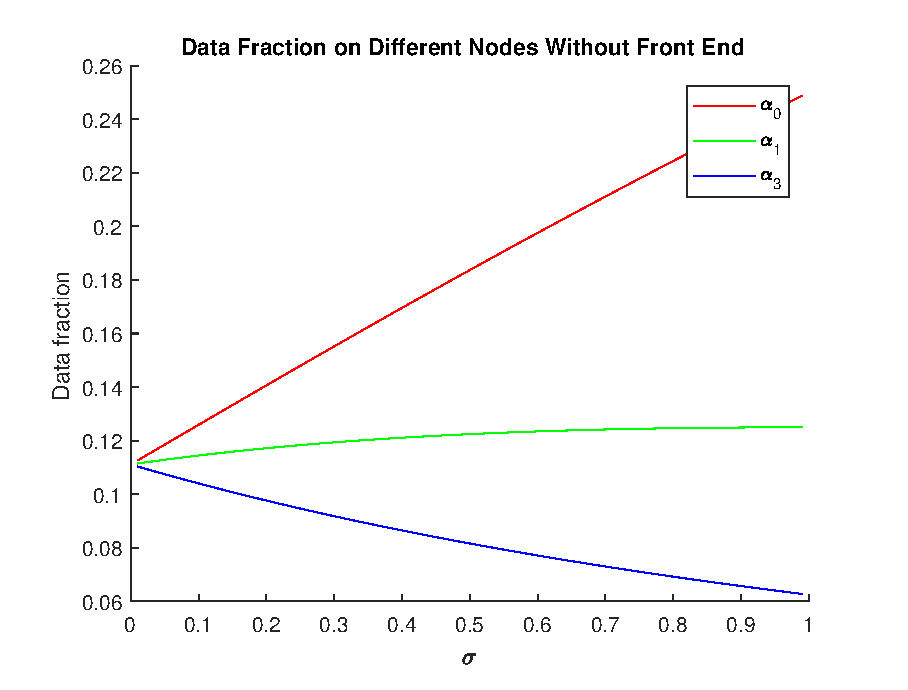
\includegraphics[width=1\columnwidth]{figure/4t4i_no_fraction.eps}
\caption{The timing diagram for 3*3 inner grid injection $P_{0}$ }
\label{fig:4t4i_no_fraction}
\end{figure}
\newpage
\subsection{Sensitivity Analysis Without Front-end Processors}
\subsubsection{Data Injection on The Corner Processor}
The simulation result of sensitivity analysis of $2*n$ regular network \Fig{2t10} is as follows:
\begin{figure}[!ht]
\centering
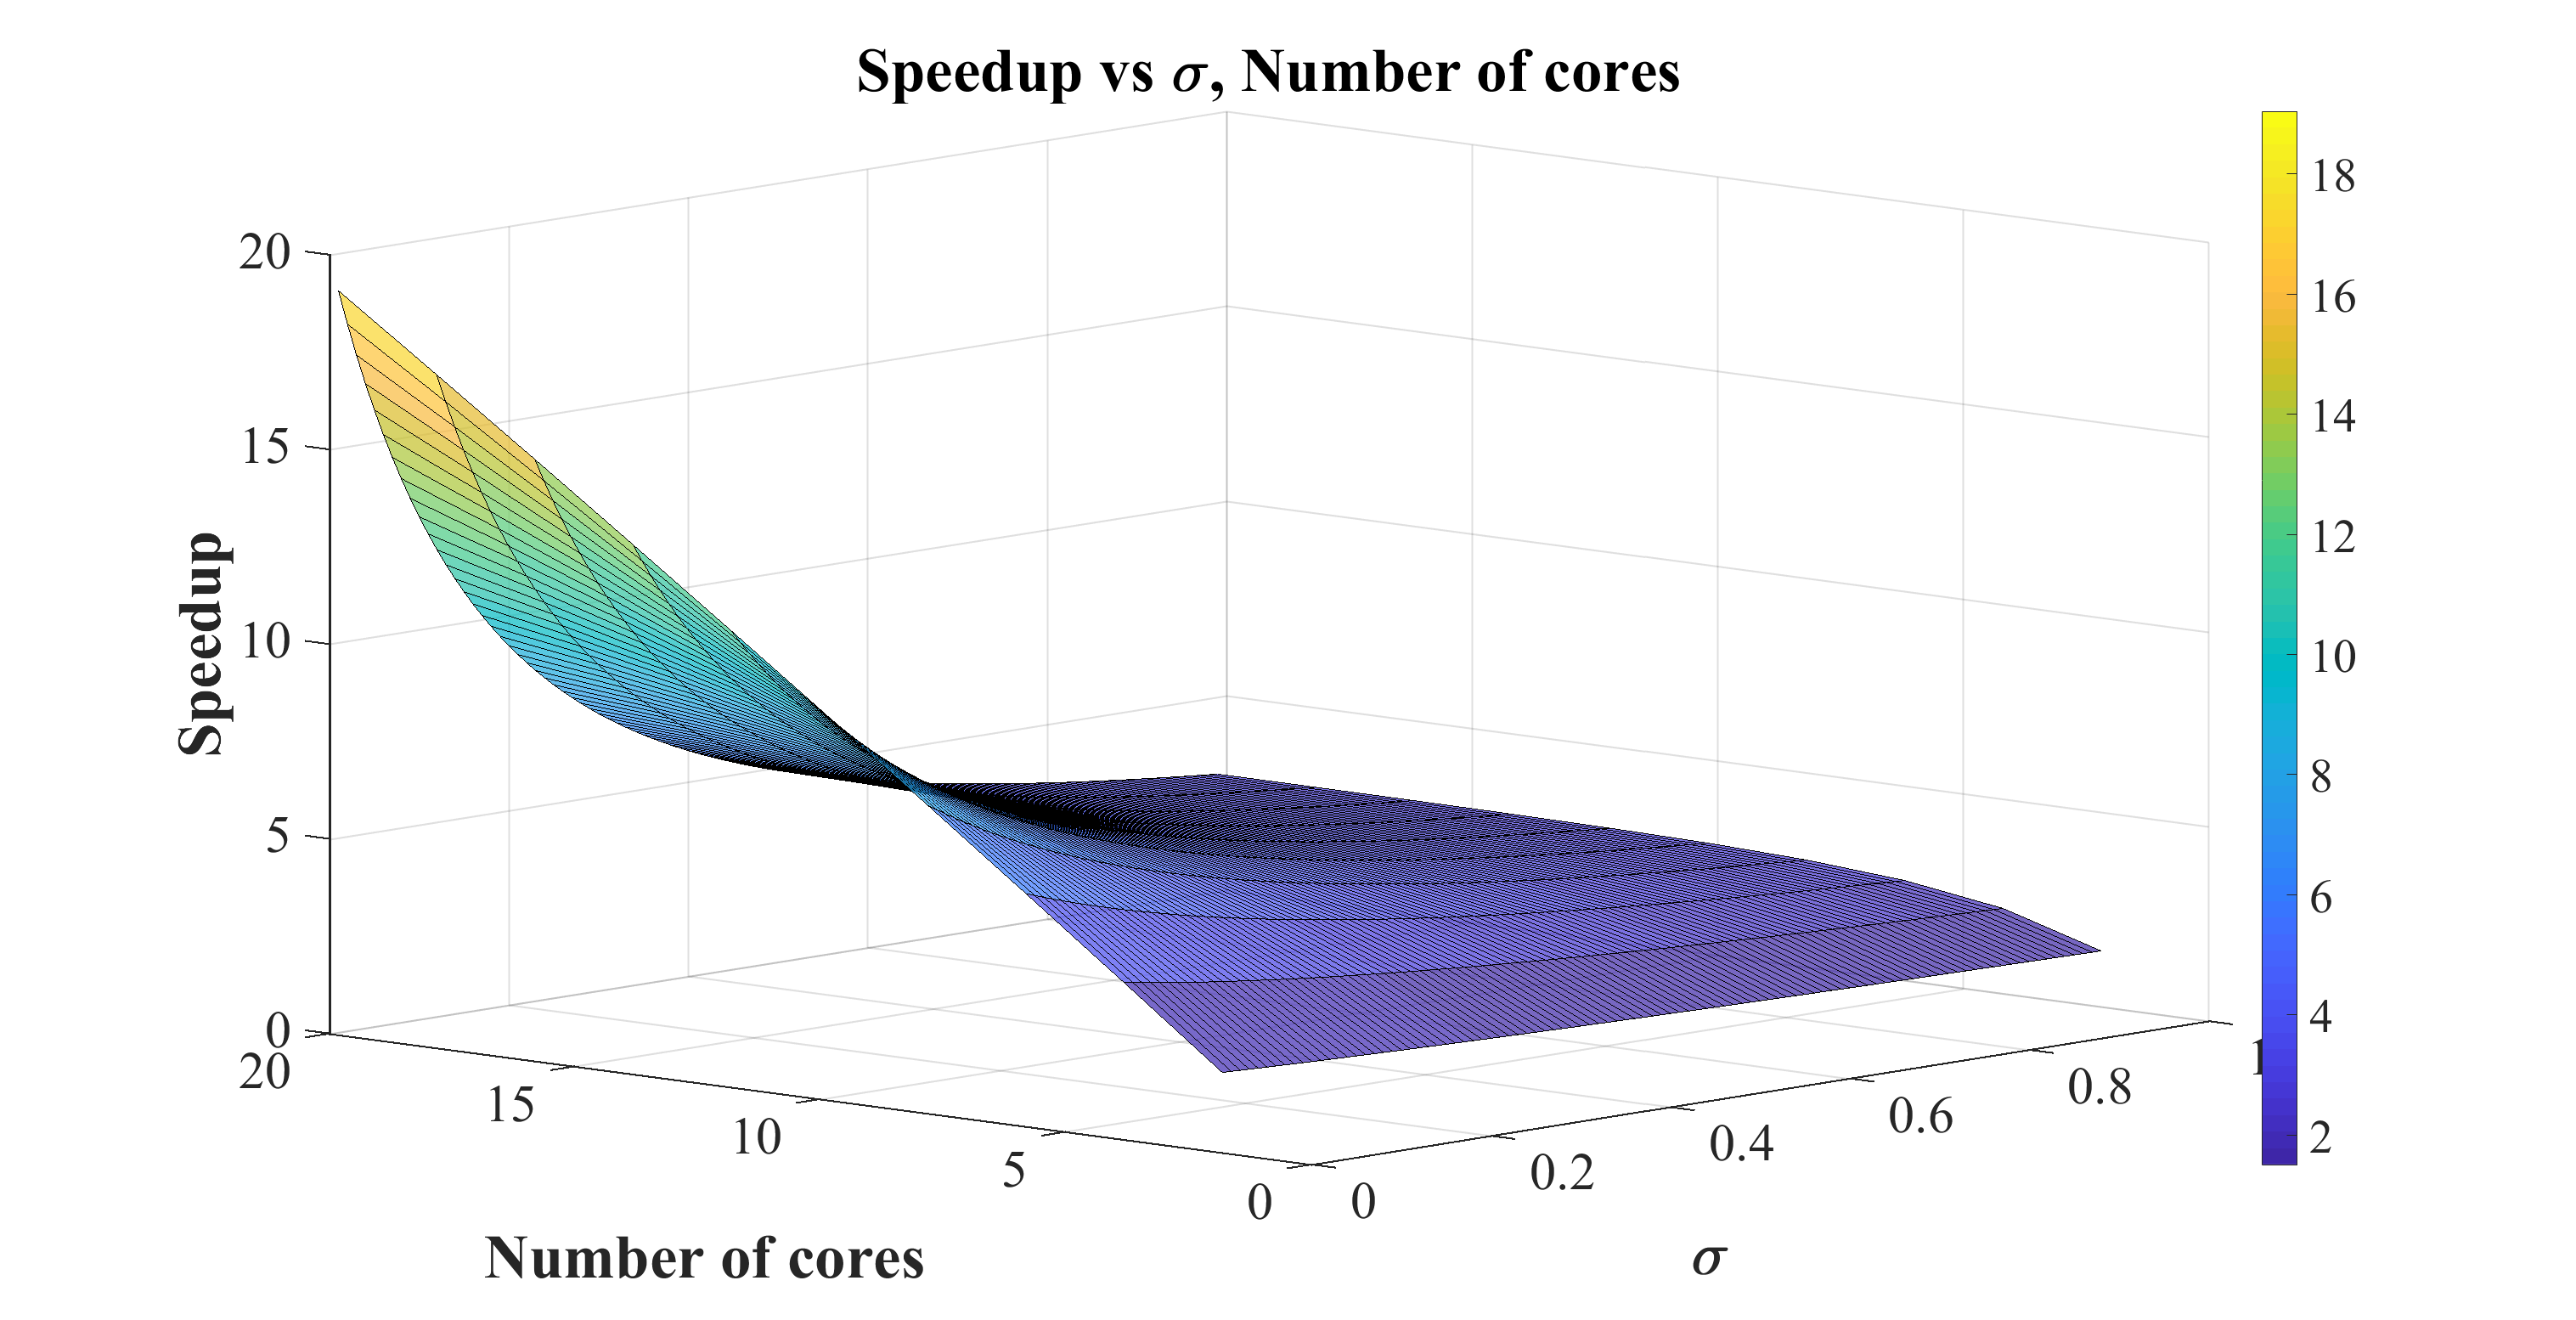
\includegraphics[width=1\columnwidth]{figure/sa2t10c_no.eps}
\caption{Sensitivity analysis result of 2*10 regular network result}
\label{fig:sa2t10c_no}
\end{figure}

The figure illustrates that if $\sigma < 0.  1$, the number of cores grow up, the speedup efficiency is likely linear increasing.   Alternatively speaking, if $\sigma < 0.  1$, the number of cores dominate the efficiency.   If the $\sigma > 0.  2$, the efficiency drops dramatically.   That is, the $\sigma$ value plays more critical role in the speedup simulation.   This important investigation benefit the multi-source assignment problem.   In addition, if the number of cores is bigger than $4$, the bottom speedup effect is about $3$ time.   
\newpage

\subsubsection{Data Injection on The Boundary Processor}
\begin{figure}[!ht]
\centering
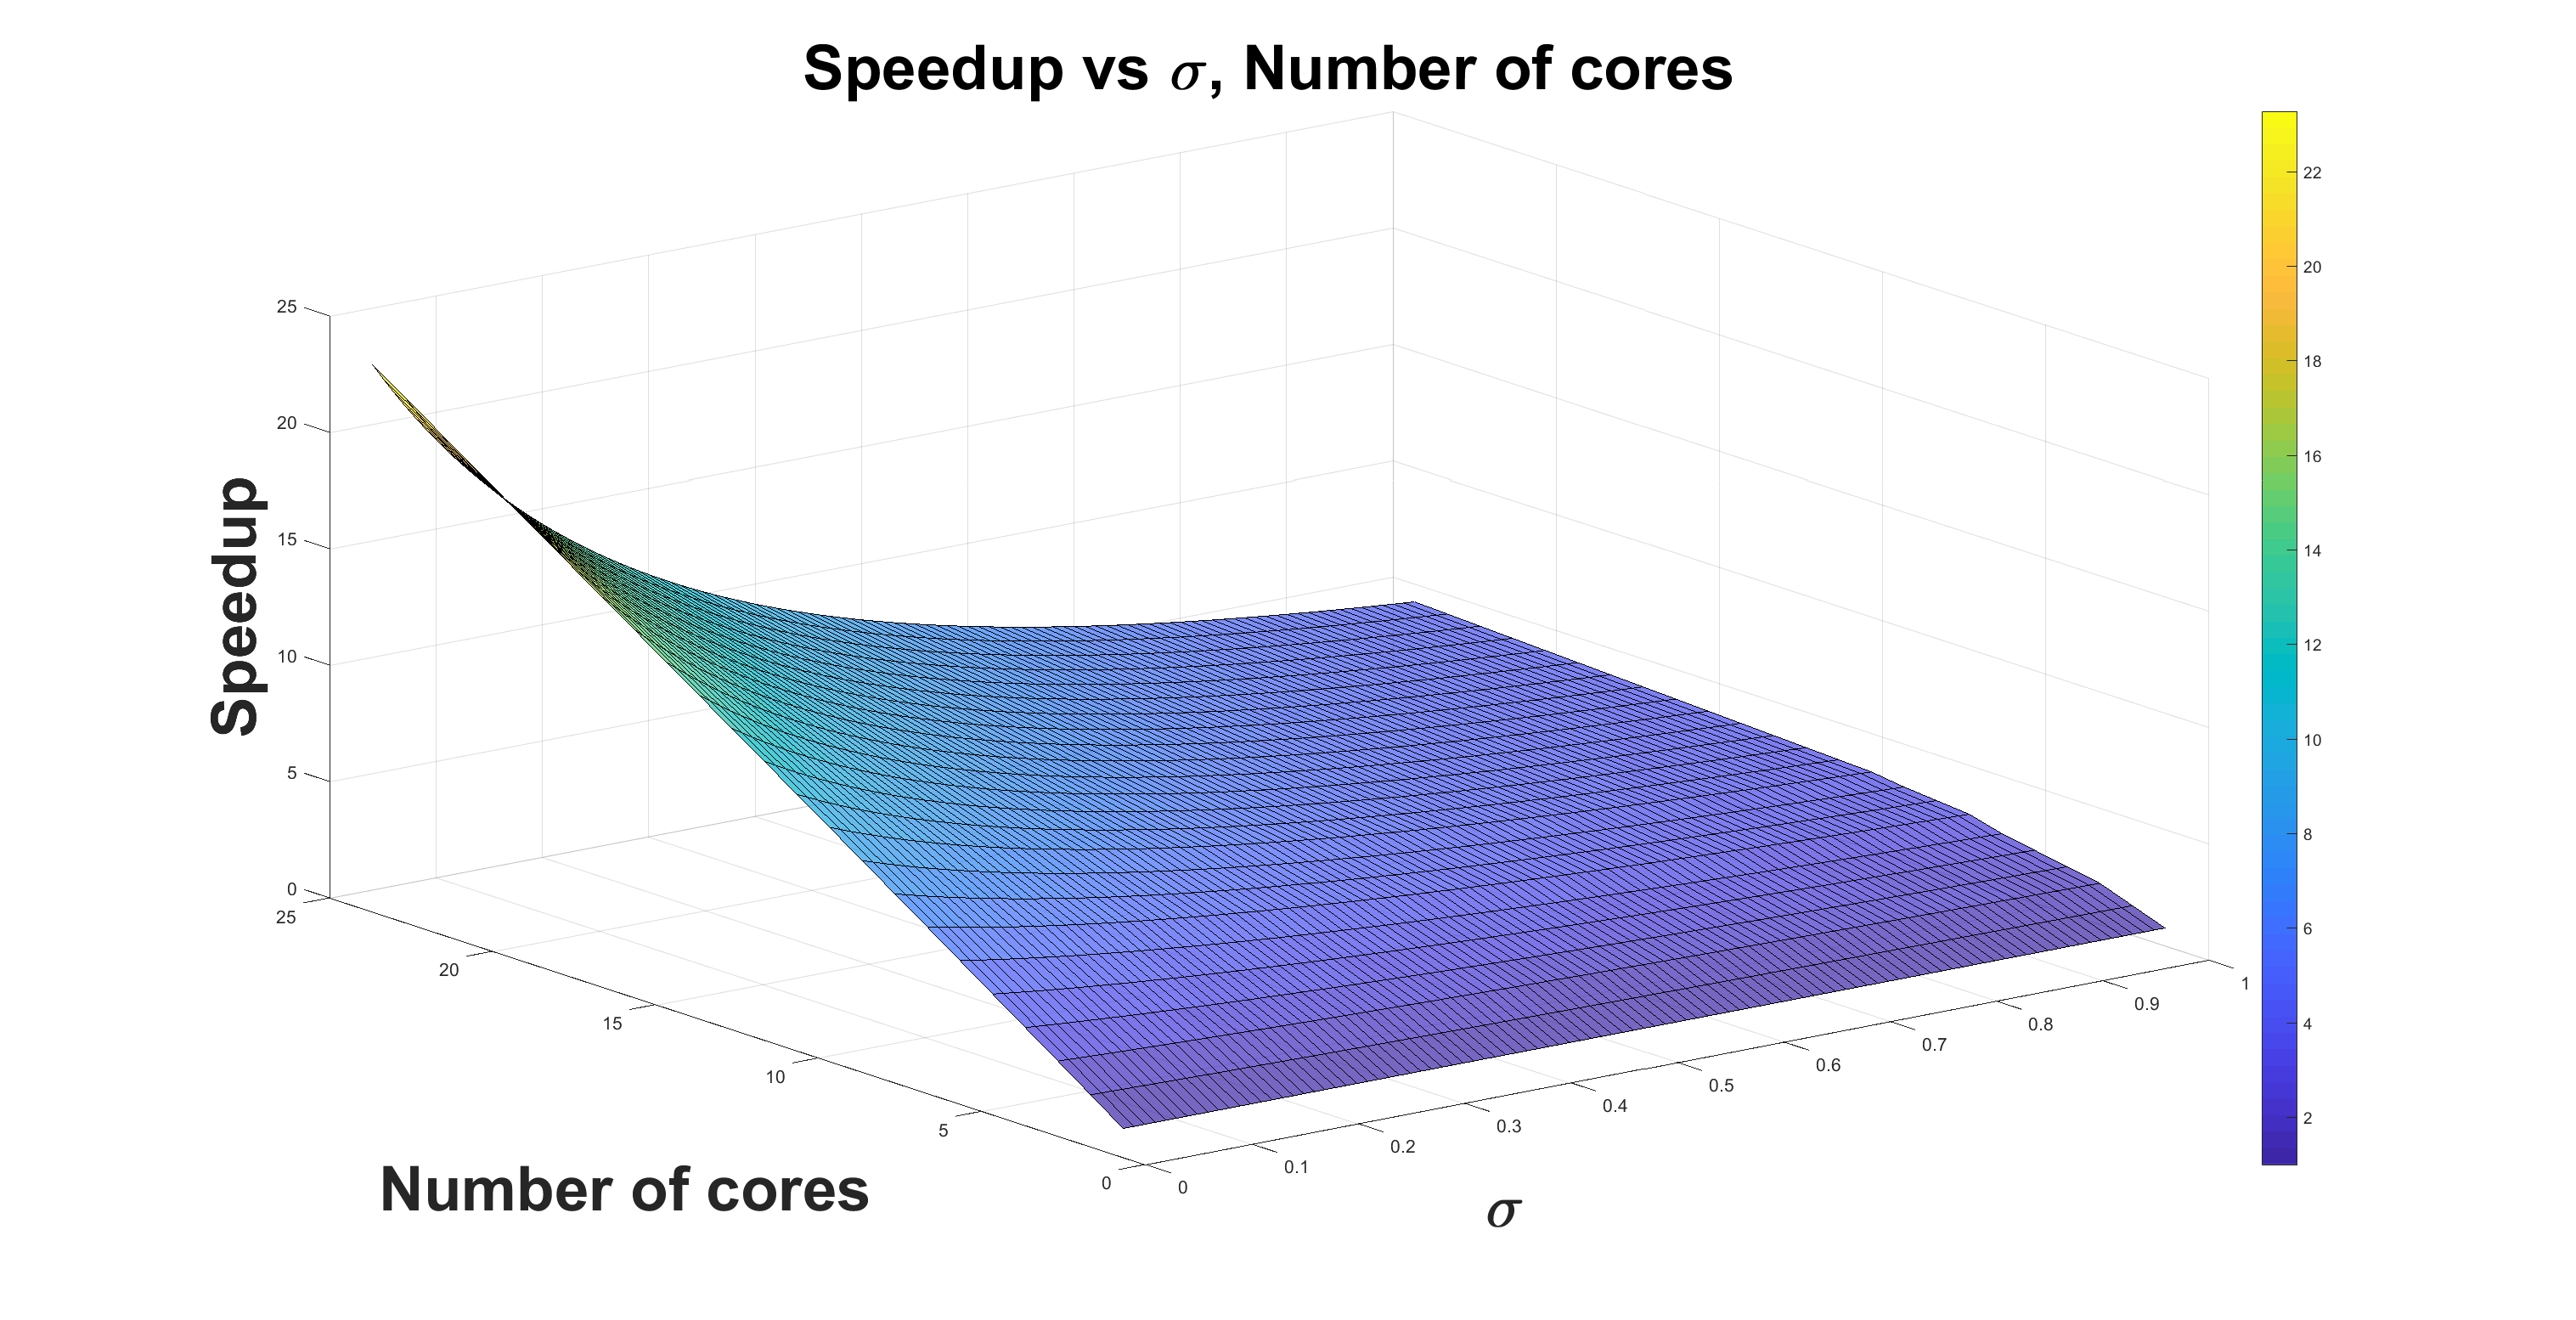
\includegraphics[width=1\columnwidth]{figure/sa3t8b_no.eps}
\caption{Sensitivity analysis result of 3*8 regular network result}
\label{fig:sa3t8b_no}
\end{figure}

\Fig{sa3t8b_no} tells the simulation result for the data injection on the boundary.  

\newpage 
\subsubsection{Data Injection on The Inner Grid Processor}
\begin{figure}[!ht]
\centering
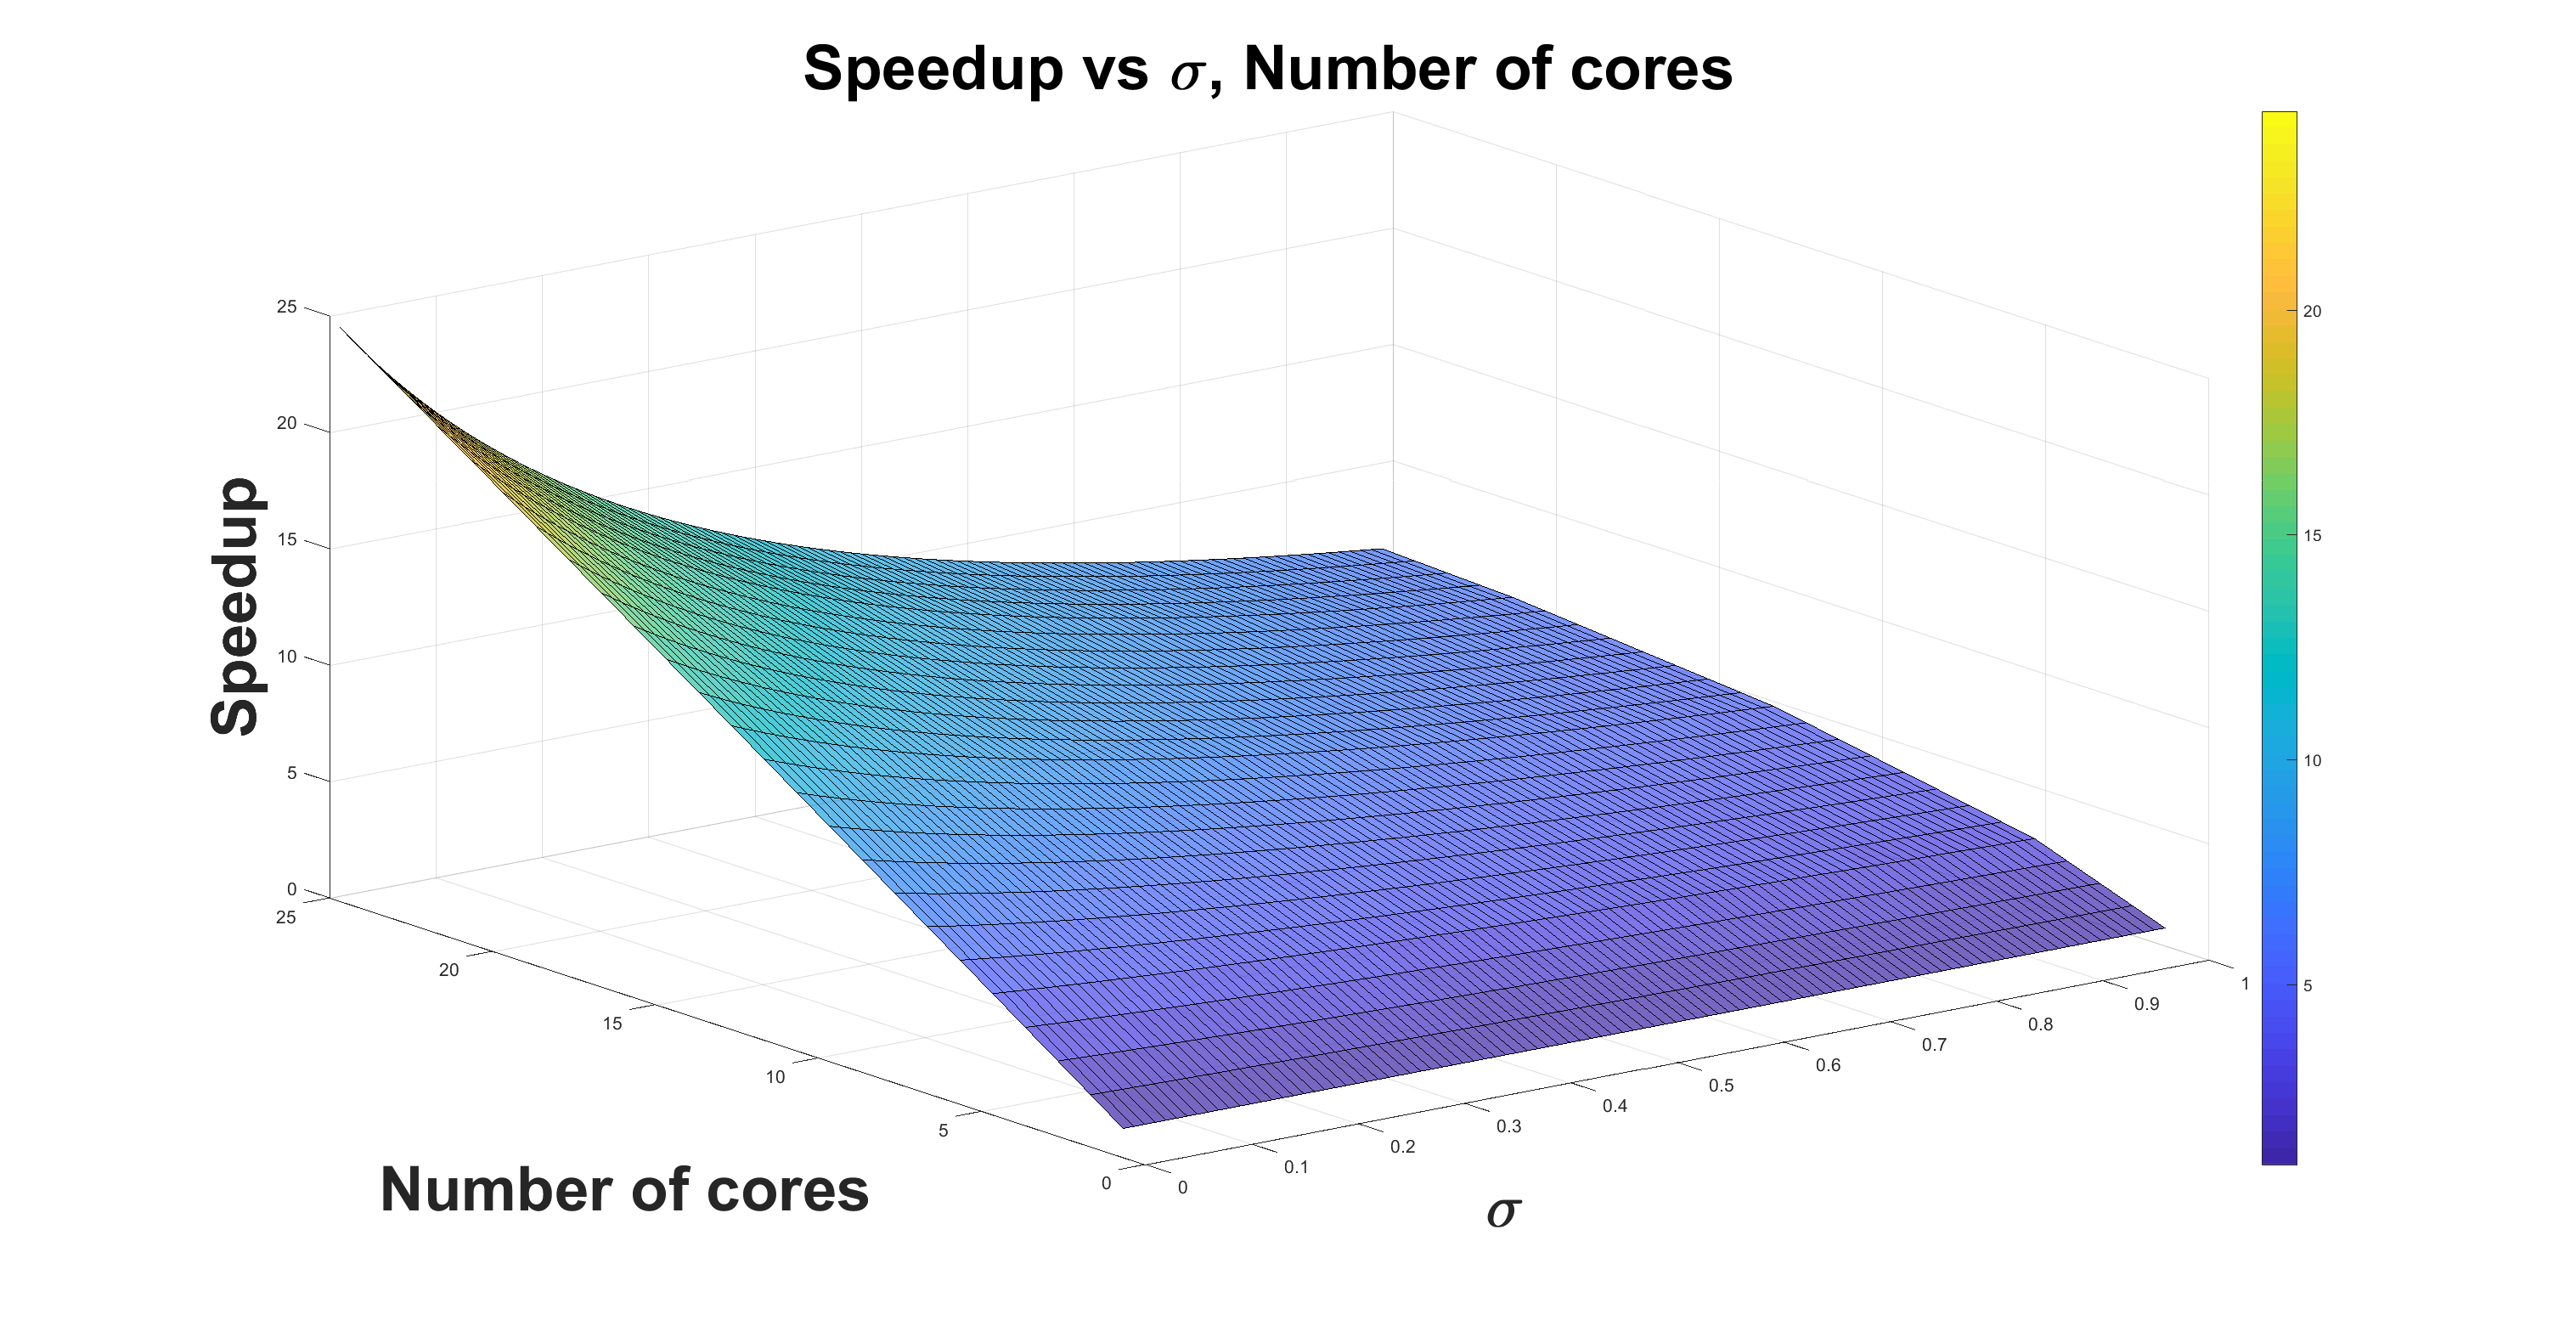
\includegraphics[width=1\columnwidth]{figure/sa5t5i_no.eps}
\caption{Sensitivity analysis result of data injection position on inner grid processor}
\label{fig:sa5t5i_no}
\end{figure}

\Fig{sa5t5i_no} displays the simulation result for the data injection position $P_{12}$.   If $\sigma < 0.1$, the speedup linear grows up and the best speedup is $24$, which happens on the $\sigma < 0.1$.   
\input{RegularMesh_no_Multi_even.tex}
\input{RegularMesh_no_Multi_no_even.tex}
       % Mathematical Models
\chapter{Numerical Implementations}
\label{Chap:Numerical}

As mentioned earlier, the simulation of parachute system involves three 
major parts: computational structure dynamics, computational fluid 
dynamics and fluid-structure interaction. 
In this chapter, we discuss the detailed numerical methods for each part. 
The data structures and many functionalities are based on \FronTierp 
library developed for front tracking method \cite{GliGroLi99a,DuFixGli05}.



\section{ODE Solvers}
\label{Sec:ODES}

\subsection{Rigid Body Rotation}
As discussed in the \Sec{RGD}, the governed equations for rigid body 
rotation are \Eqn{eulers_equation2} which is an ODE system. 
We use the fourth-order Runge Kutta method, \Eqn{4th_RK}, to solve for the 
angular velocity $\mathbf{w}$. 
\begin{eqnarray}
\begin{aligned}
u^{n+1} &= u^{n} + h(k_{1} + 2k_{2} + 2k_{3} + k_{4})/6, \\
k_{1} &= \mathscr{L}(t_n, u^{n}), \\
k_{2} &= \mathscr{L}(t_n + h/2, u^{n} + hk_{1}/2), \\
k_{3} &= \mathscr{L}(t_n + h/2, u^{n} + hk_{2}/2), \\
k_{4} &= \mathscr{L}(t_n + h, u^{n} + hk_{3}),
\end{aligned}
\label{eqn:4th_RK}
\end{eqnarray}
where $h$ is the step size and $\mathscr{L}$ is a discretization spatial
operator.

The Euler angles ($\phi$, $\theta$, $\psi$) are visually straightforward.
However, they are difficult to use in numerical computation because of the
involve of trigonometric functions in the rotation matrix 
\Eqn{rotation_matrix1}, which could lead to singularity.
For numerical purpose, we use the four-parameter representation, Euler 
parameters $\mathbf{e} = (e_{0}, e_{1}, e_{2}, e_{3})$, for propagation 
of the rigid bodies, with the constraint \Eqn{Euler_params_constraint}. 
\begin{equation}
e_0^2 + e_1^2 + e_2^2 + e_3^2 = 1
\label{eqn:Euler_params_constraint}
\end{equation}

Euler's rotation theorem states that, in three-dimensional space, any 
displacement of a rigid body such taht a point on the rigid body remain 
fixed, is equivalend to a single rotation about some axis that runs 
through the fixed point. 
This fixed point can be considered as the rotation center. 
The Euler parameters are an interpretation of Euler's rotation theorem, which
is related to an angle of rotation $\alpha$ and a unit vector along the axis 
of rotation $\mathbf{u}$. 
\begin{eqnarray}
\begin{aligned}
e_0 &= \cos(\alpha / 2) \\
\left(
\begin{array}{c}
e_1 \\ e_2 \\ e_3 \\
\end{array}
\right) &= \mathbf{u} \sin(\alpha / 2)
\end{aligned}
\label{eqn:Euler_parameters}
\end{eqnarray}
The initial status means no rotation happens.
Therefore, initially, the Euler parameters are $\mathbf{e} = (1, 0, 0, 0)$.
The relationship between the Euler parameters $\mathbf{e}$ and the angular
velocity $\mathbf{w}$ is given by
\Eqn{euler_parameters_and_angular_velocity}. 
\begin{equation}
\left(
\begin{array}{c}
\dot{e}_0 \\ \dot{e}_1 \\ \dot{e}_2 \\ \dot{e}_3 \\
\end{array}
\right) = \frac{1}{2}
\left(
\begin{array}{ccc}
-e_1 & -e_2 & -e_3 \\
e_0 & e_3 & -e_2 \\
-e_3 & e_0 & e_1 \\
e_2 & -e_1 & e_0 \\
\end{array}
\right)
\left(
\begin{array}{c}
w_1 \\ w_2 \\ w_3 \\
\end{array}
\right)
\label{eqn:euler_parameters_and_angular_velocity}
\end{equation}
As well, fourth-order Runge Kutta method \Eqn{4th_RK} is applied.

Under this circumstance, the rotation matrix $A$ can be written in terms of 
the Euler parameters $\mathbf{e}$ as
\begin{equation}
A =\left(
\begin{array}{ccc}
e_0^2+e_1^2-e_2^2-e_3^2 & 2(e_1e_2+e_0e_3) & 2(e_1e_3-e_0e_2) \\
2(e_1e_2-e_0e_3) & e_0^2-e_1^2+e_2^2-e_3^2 & 2(e_2e_3+e_0e_1) \\
2(e_1e_3+e_0e_2) & 2(e_2e_3-e_0e_1) & e_0^2-e_1^2-e_2^2+e_3^2 \\
\end{array}
\right)
\label{eqn:rotation_matrix}
\end{equation}
The transpose $A^T$ is also the inverse of the rotation matrix $A$. 
$x' = Ax$ represents the rotation process from the world/space coordinates 
system to the body-fixed coordinates system, and $x = A^Tx'$ does the 
opposite process. 
Because the order of rotation in 3 dimensional cases matters, when 
propagating the rigid body from time $t_n$ to $t_{n+1}$, we have the 
following equation.
\begin{equation}
x_{n+1} = A^T_{n+1} A_n x_n
\end{equation}
The subscripts $n$ and $n+1$ are the time step index. This means we always 
first convert to the body-fixed coordinates system before apply the updated 
rotation matrix. 



\subsection{Spring Solver}
\label{Sec:SS}
For the spring-mass model, explicit integration with fourth order 
Runge-Kutta method \Eqn{4th_RK} is adopted to solve the ODE system 
\Eqn{sm_ODEs}.

The explicit scheme requires us to pay attention to the numerical stability 
of the spring solver. 
Based on the previous analysis and numerical verification in 
\cite{LiChernKimLi12, KimLiLi12}, the spring-mass system is a conservative 
system without external forces, and there exists an upper bound for the 
eigenfrequency of the oscillation 
\begin{equation}
w_{max} \leq \sqrt{\frac{2Mk}{m}}, 
\label{eqn:eigenfrequency}
\end{equation}
where $M$ is the maximum number of neighbors that a spring vertex has, $k$ 
is the tensile stiffness and $m$ is the point mass. 
The Delingette's modification adds variation to the spring model, but the 
upper bound is still valid except that the maximum tensile stiffness is used 
in \Eqn{eigenfrequency} instead. 
Therefore, for stability and accuracy purpose, we choose $w_{max}h < 0.1$ for 
simulations.



\section{PDE Solvers}
\label{Sec:PDES}

There have been many techniques to solve the governed equations that describes 
the motion of the fluid. 
For compressible fluid, \Eqn{Euler_eqns_con}, since it is a hyperbolic system, 
we apply the 5th Weighted Essentially Non-Oscillatory (WENO) scheme. 
For incompressible fluid, a pressure correction projection method is used, 
which can achieve second order accuracy. 

\subsection{WENO Scheme}
High-order numerical methods have been widely used to effectively resolve 
complex flow features such as turbulent or vertical flows 
\cite{Ekaterinaris2005192}. 
High-order shock-capturing schemes such as the Essentially Non-Oscillatory 
(ENO) and Weighted ENO (WENO) \cite{Liu1994200,Jiang1996202} schemes not 
only make the computational fluid dynamics (CFD) solvers get rid of 
extremely fine mesh for complex flows, but also perfectly eliminate the 
oscillations near discontinuities. 
WENO scheme is used to reconstruct the spatial derivative term and then the 
hyperbolic system is converted to an ODE system and propagated by 3rd order 
Total Variation Diminishing (TVD) Runge-Kutta method. 

Take one-dimensional Euler equation \Eqn{1d_Euler} for example
\begin{equation}
\mathbf{U}_{t}+\mathbf{F}\left(\mathbf{U}\right)_{x} = 0
\label{eqn:1d_Euler}
\end{equation}
where 
\begin{equation}
\mathbf{U} = 
\left(
\begin{array}{c}
\rho\\ \rho u\\ E
\end{array}
\right),\ 
\mathbf{F}(\mathbf{U}) = 
\left(
\begin{array}{c}
\rho u\\ \rho u^{2}+p\\ (E+p)u
\end{array}
\right)
\end{equation}
\begin{equation}
E = \rho (e+\frac{u^{2}}{2}),\ p = \rho e (\gamma - 1)
\end{equation}
$\rho$, $u$, $P$, $e$ and $\gamma$ denote the density, velocity,
pressure, internal energy per unit mass and ratio of specific heats,
respectively. The Jacobian matrix of the Euler equations is defined as 
\begin{equation}
\mathbf{A} = \frac{\partial \mathbf{F}(\mathbf{U})}{\partial \mathbf{U}}
\end{equation}
The eigenvalues of the Jacobian matrix $A$ are 
\begin{equation}
\lambda_{1} = u-c,\ \lambda_{2}=u,\ \lambda_{3}=u+c
\end{equation}
where $c=\sqrt{\frac{\gamma p}{\rho}}$ is the sound speed, and the
corresponding right eigenvectors are 
\begin{equation}
\mathbf{r}_{1} = 
\left(
\begin{array}{c}
1\\ u-a\\ H-ua
\end{array}
\right),\ 
\mathbf{r}_{2} = 
\left(
\begin{array}{c}
1\\ u\\ \frac{u^{2}}{2}
\end{array}
\right),\ 
\mathbf{r}_{3} = 
\left(
\begin{array}{c}
1\\ u + a\\ H + u a
\end{array}
\right)
\label{eqn:Euler_eigvec}
\end{equation}
where $H$ is the total specific enthalpy, which is related to the
specific enthalpy $h$ and other variables, namely 
\begin{equation}
H = \frac{E + p}{\rho} = \frac{1}{2}u^{2} + h,\ h = e + \frac{P}{\rho}
\end{equation}
We denote the matrix whose columns are eigenvectors in \Eqn{Euler_eigvec} by 
\begin{equation}
\mathbf{R} = \left(\mathbf{r}_{1},\mathbf{r}_{2},\mathbf{r}_{3}\right)
\end{equation}
and denote $\mathbf{L} = \mathbf{R}^{-1}$. The eigenvalue decomposition
of $\mathbf{A}$ is 
\begin{equation}
\mathbf{A} = \mathbf{R \Lambda L}
\end{equation}
where $\mathbf{\Lambda} = diag(u-c,u,u+c)$. Then, \Eqn{1d_Euler} can be 
transformed as 
\begin{equation}
\mathbf{(LU)}_{t} + \Lambda(\mathbf{LU})_{x} = 0
\label{eq:1d_transEuler}
\end{equation}
which consists of three independent one-dimensional hyperbolic equations. 
The advection term in each equation can be reconstructed using WENO scheme 
then solved by advection solver. 

\subsection{Projection Method}
Projection method is an effective way to numerically solve the time-dependent 
incompressible fluid flow problems. 
We apply the pressure-Poisson version of projection method 
\cite{Chorin68, KimMoin85, Brown2001accurate} is adopted to solve the 
Navier-Stokes \Eqn{navierstoke_eqns}. 
\begin{itemize}
\item step 1: Solve for the intermediate velocity $u^*$.
    \begin{eqnarray}
    \begin{aligned}
    \frac{u^* - u^n}{\Delta t} + \frac{1}{\rho} \nabla q &= -[(u \cdot \nabla) u]^{n + \frac{1}{2}} + \frac{\mu}{2\rho} \nabla^2 (u^* + u^n), \\
    B(u^{*}) &= 0, 
    \end{aligned}
    \label{eqn:projection_1}
    \end{eqnarray}
    where $q$ represents an approximation of $p^{n+\frac{1}{2}}$ and 
    $B(u^{*})$ is the boundary condition for $u^{*}$. 
    The term $[(u \cdot \nabla) u]^{n + \frac{1}{2}}$ represents an 
    approximation of the advection term, which is done by WENO scheme. 
    Crank-Nicolson scheme is used to solve this advection-diffusion equation. 
\item step 2: Perform the projection
    \begin{eqnarray}
    \begin{aligned}
    u^* &= u^{n+1} + \Delta t \nabla \phi^{n+1} \\
    \nabla \cdot u^{n+1} &= 0
    \end{aligned}
    \label{eqn:projection_2}
    \end{eqnarray}
    using the boundary conditions consistent with $B(u^{*}) = 0$ and 
    $u^{n+1}|_{\partial \Omega} = u^{n+1}_{b}$. 
    After elimimating $u^{n+1}$, the above two equation becomes a Poisson 
    equation of $\phi$ which is solved by iterative methods. 
\item step 3: Update the pressure.
    \begin{equation}
    p^{n+\frac{1}{2}} = q + \phi^{n+1} - \frac{\mu \Delta t}{2\rho} \nabla^2 \phi^{n+1}.
    \label{eqn:projection_3}
    \end{equation}
    The last term in the above equation gives the second-order accuracy. 
\end{itemize}



\section{Fluid-Structure Interaction}
\label{Sec:FSI}
The interaction between fluid and fabric surface structure is a crucial part 
of the parachute system simulation. 
As mentioned above, the canopy experiences three forces, the gravitational 
force due to the weight of the material, the fluid-generated force due to 
the pressure difference on two sides of the canopy, and the internal spring 
force (both restoring force and friction force). 

\subsection{Force Calculation}
We handle this by the impulse method \cite{KimLiLi12} on the \FronTierp 
platform. 
For each mass point in the spring system, we divide the impulse into three 
components, the gravitational impulse, the fluid impulse and the internal 
impulse due to the spring system, that is, 
\begin{equation}
\mathbf{I}_i^C = \mathbf{I}_{gi}^C + \mathbf{I}_{pi}^C + \mathbf{I}_{si}^C.
\end{equation}
Since no fluid interaction with the string chord is considered in our model, 
the impulse splitting for these mass points is 
\begin{equation}
\mathbf{I}_i^S = \mathbf{I}_{gi}^S + \mathbf{I}_{si}^S.
\end{equation}
The gravitational impulse is straightforward and has the same formula for 
the spring vertex on both the canopy and string chords. 
\begin{equation}
\mathbf{I}_{gi} = \int_{0}^{t} m_{i} \mathbf{g} ds.
\end{equation}
The fluid impulse is 
\begin{equation}
\mathbf{I}_{pi} = \int_{0}^{t} \sigma (p^{-} - p^{+}) \mathbf{n} ds, 
\end{equation}
where $\sigma$ is the mass density of canopy per unity area, $p^{-}$ and 
$p^{+}$ are the pressure on the lower side and upper side of the canopy, 
and $n$ is the unit normal vector pointing from lower to upper side of the 
canopy. 
This follows \cite{Kalro00} for its simplicity. 
A more accurate calculation should also include the velocity shear near the 
canopy surface and stress to the surface. 

For the calculation of the reacting impulse between the canopy and the 
fluid, we apply the immersed boundary method which treats the reaction of 
the canopy as the normal force approximated by the smoothed delta function, 
that is Peskin's delta function, 
\begin{equation}
\mathbf{f}(\mathbf{x}, t) = \int \mathbf{F}(\mathbf{x}, t) \delta(x - \mathbf{X}(s, t)) ds.
\label{eqn:peskin_delta}
\end{equation}
The difference is that we use the impulse of the mass point as a result 
of the superposition of three forces from the spring system, 
\begin{equation}
\mathbf{F}(\mathbf{x}_{i}, t) = d(\mathbf{I}_{g} + \mathbf{I}_{p} + \mathbf{I}_{s}) / dt.
\end{equation}
Numerically, the surface force is the product of the normal component of 
the acceleration and mass density at the canopy surface 
\begin{equation}
\mathbf{F}(s, t) = \rho_{c} (\mathbf{a} \cdot \mathbf{n}) \mathbf{n}, 
\end{equation}
where $\mathbf{n}$ is the unit normal vector on the canopy surface, and 
$\rho_{c}$ is the mass density of canopy per unit area.

\subsection{Local Index Coating}
Our simulation of the parachute system is performed on the \FronTierp 
platform, which uses the front tracking method. 
This method is widely used for tracing the fluid interface in multi-phase 
flow problems, such as the Rayleigh-Taylor instability 
\cite{GliMcBMen86, GliLiMen90}, Richtmyer–Meshkov instability 
\cite{GarGliGro88}, and the jet problems \cite{GliKim04, GliLiOh02}. 
In problems like these, the fluid interface is topologically a manifold, 
the two sides of each surface are the boundaries of two separate domains. 
However, it is not the case in the simulation of parachute system where 
the canopy surface is thinness and forms an open boundary. 
You cannot tell which side of the canopy surface it belongs when a point is 
far away from it. 
But, for points that are sufficiently close to the canopy surface, we can 
still distinguish which side it belongs. 

The reason that we pay attention to this is that the local side information 
of space points that are near the canopy surface contributes to the 
calculation of the pressure difference, and thus the fluid force on the 
canopy. 
The pressure on two sides of the canopy surface is not continuous and it 
should be interpolated using the pressure information on its own side, which 
is realized by locally mesh coating algorithm.
Assign the domain in which the canopy is immersed with index $l$, and the 
local index coating algorithm follows three steps: 
\begin{itemize}
\item For any grid point $P$ with a distance $d \leq h$ away from the canopy, 
where $h$ is the grid spacing, find the nearest point on the canopy surface 
(\FronTierp is well equipped with these geometry functions) $P_{s}$. 
Using the sign of the scalar product $\overline{PP_{s}} \cdot \mathbf{n}_{s}$, 
we can determine the side of the point. 
Reassign domain index to $l-1$ if the point $P$ is on the negative side, 
otherwise reassign the index to $l+1$.
\item Reassign any grid point adjacent to a point indexed $l-1$ to the same; 
reassign any grid point adjacent to a point indexed $l+1$ to the same. 
Repeat this assignment for three sweeps. 
The resulting landscape of the grid index will look like \Fig{local_coating}. 
\item The interpolation of side-sensitive variables will use grid points of 
the same locally coated index.
\end{itemize}
\begin{figure}[!ht]
\centering
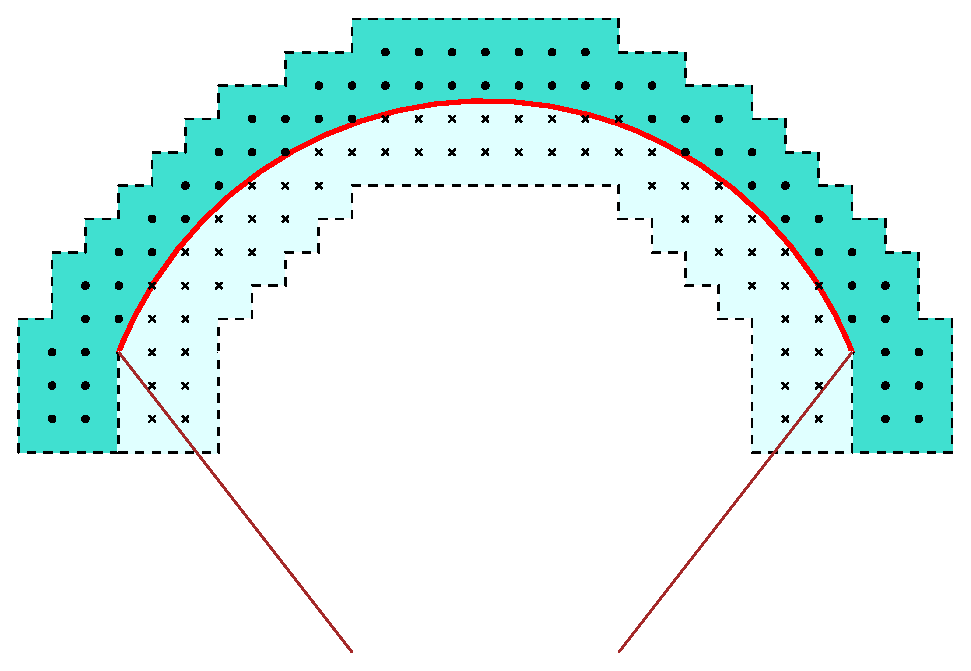
\includegraphics[width=0.7\columnwidth]{figures/local_coating}
\caption{The parachute canopy is an open surface and cannot separate the 
space into sub-domains. But we can still coat different index for mesh 
cells close to the surface using the local geometrical information. The 
light and dark shaded polygons represent the sets of mesh cells on the 
positive and negative sides of the canopy, respectively. An interpolation 
is carried out on vertex of the same color.}
\label{fig:local_coating}
\end{figure}



\section{Collision Features}
\label{Sec:CF}
Collision module for structures is a new feature added to the computational
framework.
With triangulized meshes, the proximity and collision checks can be broken
down into two major cases: a point against a triangle, an edge against
another edge.
For example, when there is collision detected between a pair of triangles,
15 tests need to be done in total.
\begin{itemize}
\item each point of one triangle against the other triangle
\item each edge of one triangle against each edge of the other triangle
\end{itemize}
When strings are taken into account, the comparison pairs can be not only
triangle-triangle, but also edge-edge and edge-triangle, because a string is
represented by a group of connected edges.
Similarly, there is 1 check for a edge-edge pair, and 5 checks for a
edge-triangle pair.

When there are movable rigid bodies involved in collision, we make use of the
impact zone technique which is first proposed in \cite{Provot1997} and further
developed in \cite{Bridson2002collsn}.
This technique was initially proposed to deal with multiple collisions and
maintain collision consistency.
The idea of the impact zone technique is to collect the points in multiple
collisions into separated zones, and treat them as rigid bodies.
Therefore, we can construct each movable rigid body as one independent impact
zone before resolving collisions.
Similar handling as cloth is applied to movable rigid bodies, but we adopted
some differences.
\begin{itemize}
\item The impulse added to each mass point due to collision consists of two
components: inelastic impulse and elastic impulse.
    \begin{itemize}
    \item If the two structures that collid are the same type, i.e. two
    elastic structures or two rigid structures, the inelastic impulse is
    distributed according to the mass
    \begin{equation}
    I_{in, i} = m_{1}m_{2}v_{n} / (m_1 + m_2); 
    \end{equation}
    otherwise, it is distributed evenly
    \begin{equation}
    I_{in,i} = 0.5 m_{i}v_{n}. 
    \end{equation}
    In above, $m_{1}$ and $m_{2}$ are masses and $v_{n}$ is the magnitude of
    relative velocity in the normal direction.
    \item When there is elastic structure(s) involved in the collision,
    the elastic impulse performs like a repulsion due to the elasticity
    \begin{equation}
    I_{el, i} = -min(\Delta t k d, m_{i}(0.1d/\Delta t - v_{n})); 
    \end{equation}
    otherwise, it is the case of two rigid structures
    \begin{equation}
    I_{el, i} = cr I_{in, i}. 
    \end{equation}
    Here, $d$ is the overlap length, $k$ is the string stiffness and $cr$ is
    the restitution coefficient.
    \end{itemize}
\item Whenever an impulse acts on some point on a movable rigid body, it is
spread, via impact zone connection, to all the points on that rigid body.
This is the constraint to maintain the geometric shape of the rigid bodies.
\item The impulse due to cloth-involved collision and that due to rigid
collision are recorded and averaged separately.
Because there will be much more collision detected with cloth, while fewer
between rigid bodies.
\end{itemize}



\newpage
   % Numerical Methods
\chapter{Hypercube Network}
\section{With Front-end Scenario}
The hypercube topology has two nodes along each dimension and $\log_2 n$ dimensions.  The construction of a hypercube goes as follows, in general a $d-$dimensional hypercube is constructed by connecting corresponding nodes of two $(d-1)$ dimensional hypercubes \Fig{hypercube_basic}.\\

\begin{figure}[!ht]
\centering
\includegraphics[width=1\columnwidth]{figure/hypercube_basic.JPG}
\caption{Hypercube in $0$, $1$, $2$, $3$ dimension. \cite{Informatik5}}
\label{fig:hypercube_basic}
\end{figure}

In this work, we have two tasks as follows :
\begin{itemize}
\item One data injection, we propose a method of finding an optimal distribution of a divisible job among a cluster of processors connected by communication links and forming a hypercube network.  The methodology we apply is similar to the flow matrix technique.\\
\item Sensitivity analysis of the hypercube structure by adding more processors or dimensions.
\item The multi-source sub-optimal algorithms to speedup job execution.
\begin{itemize}
\item The data injection fractions are even.
\item The data injection fractions are different with each other.
\end{itemize}
\end{itemize}

\subsection{Data Injection On The Grid Processor}
For the hypercube of dimension $d$ there are $2^{d}$ processor in the system.  Each of the processors has direct links to $d$ neighbors.  A method of naming the processors is to use label consisting of a binary string $d-$ position long.  Further, the label of a processor is a binary number from the interval $[0, 2^{d}-1]$

To address the qualitative model of computation, the critical problem is to calculate the number of processor on each $D_{i}$.  Each node is connected by link and the hamming distance of their's label is $1$.  According to the lemma of \cite{blazewicz1995scheduling}, \\

\begin{lemma}
In each layer $i$ of $d-$dimensional hypercube, there are ${n \choose i}$ processors each of which can be accessed through $i$ communications links and is capable of transmitting to $d-i$ still idle processors.
\end{lemma}

According to a $2-D$ hypercube \Fig{2t2}, the flow matrix is  
\begin{equation}
{
A = \left[ \begin{array}{ccc}
{2 \choose 0} & {2 \choose 1} & {2 \choose 2}\\
1 & -1 & 0\\
0 & \sigma-1 & 1
\end{array} 
\right ]
=
\left[ \begin{array}{ccc}
1 & 2 & 1\\
1 & -1 & 0\\
0 & \sigma-1 & 1
\end{array} 
\right ]
} 
\end{equation}
, which is investigated in Regular Network Chapter.\\

According to a $3-D$ hypercube, the flow matrix is \\

\begin{equation}
{
A = \left[ \begin{array}{cccc}
{3 \choose 0} & {3 \choose 1} & {3 \choose 2} & {3 \choose 3}\\
1 & -1 & 0 & 0\\
0 & \sigma-1 & 1 & 0\\
0 & \sigma-1 & \sigma & 1\\
\end{array} 
\right ]
=
\left[ \begin{array}{cccc}
1 & 2 & 2 & 1\\
1 & -1 & 0 & 0\\
0 & \sigma-1 & 1 & 0\\
0 & \sigma -1 & \sigma & 1
\end{array} 
\right ]
} 
\end{equation}
\\

The speedup is $\left | -\det A \right |$.
\newpage
A general case, $D-$dimension network, the flow matrix is :
\begin{equation*}
     {A = \left[ \begin{array}{ccccccc}
{n \choose 0} & {n \choose 1} & {n \choose 2}  & \cdots & {n \choose n-2} &{n \choose n-1} & {n \choose n} \\
1 & -1 & 0 & \cdots& 0 & 0 & 0\\
0 & \sigma-1 & 1 & \cdots & 0 & 0 & 0 \\
0 & \sigma-1 & \sigma & 1 & 0 & \cdots & 0 \\
0 & \sigma-1 & \sigma & \sigma & 1 & 0 & 0 \\
\vdots & \vdots & \vdots  &   \vdots & \ddots & \ddots\\
0 & \sigma-1 & \sigma & \cdots & \sigma & \sigma & 1
\end{array} 
\right ]}
\end{equation*}




\subsection{Sensitivity Analysis With Front-end Processors}
\newpage
\input{Hyper_Multi_even.tex}
\input{Hyper_Multi_no_even.tex}
\section{Without Front-end Scenario}
In this work, we have two tasks as follows :
\begin{itemize}
\item One data injection, we propose a method of finding an optimal distribution of a divisible job among a cluster of processors connected by communication links and forming a hypercube network.  The methodology we apply is similar to the flow matrix technique.\\
\item Sensitivity analysis of the hypercube structure by adding more processors or dimensions.
\item The multi-source sub-optimal algorithms to speedup job execution.
\begin{itemize}
\item The data injection fractions are even.
\item The data injection fractions are different with each other.
\end{itemize}
\end{itemize}

\subsection{Data Injection On The Grid Processor}

According to a $2-D$ hypercube \Fig{2t2}, the flow matrix is  
\begin{equation}
{
A = \left[ \begin{array}{ccc}
{2 \choose 0} & {2 \choose 1} & {2 \choose 2}\\
1 & -(\sigma + 1) & 0\\
1 & -\sigma & -(\sigma + 1)
\end{array} 
\right ]
=
\left[ \begin{array}{ccc}
1 & 2 & 1\\
1 & -(\sigma + 1) & 0\\
1 & -\sigma & -(\sigma + 1)
\end{array} 
\right ]
} 
\end{equation}
, which is investigated in Regular Network Chapter.\\

According to a $3-D$ hypercube, the flow matrix is \\

\begin{equation}
{
A = \left[ \begin{array}{cccc}
{3 \choose 0} & {3 \choose 1} & {3 \choose 2} & {3 \choose 3}\\
1 & -(\sigma + 1) & 0 & 0\\
1 & -\sigma & -(\sigma + 1) & 0\\
1 & -\sigma & -\sigma & -(\sigma + 1)\\
\end{array} 
\right ]
=
\left[ \begin{array}{cccc}
1 & 2 & 2 & 1\\
1 & -(\sigma + 1) & 0 & 0\\
1 & -\sigma & -(\sigma + 1) & 0\\
1 & -\sigma & -\sigma & -(\sigma + 1)\\
\end{array} 
\right ]
} 
\end{equation}
\\

The speedup is $\left | -\det A \right |$.
\newpage
A general case, $D-$dimension network, the flow matrix is :
We use $\sigma^{\star}$ to represents $-(\sigma + 1)$.
\begin{equation*}
     {A = \left[ \begin{array}{ccccccc}
{n \choose 0} & {n \choose 1} & {n \choose 2}  & \cdots & {n \choose n-2} &{n \choose n-1} & {n \choose n} \\
1 & \sigma^{\star} & 0 & \cdots& 0 & 0 & 0\\
1 & -\sigma & \sigma^{\star} & \cdots & 0 & 0 & 0 \\
1 & -\sigma & -\sigma & \sigma^{\star} & 0 & \cdots & 0 \\
1 & -\sigma & -\sigma & -\sigma & \sigma^{\star} & 0 & 0 \\
\vdots & \vdots & \vdots  &   \vdots & \ddots & \ddots\\
1 & -\sigma & -\sigma & \cdots & -\sigma & -\sigma & \sigma^{\star}
\end{array} 
\right ]}
\end{equation*}
\subsection{Sensitivity Analysis Without Front-end Processors}
\newpage
\input{Hyper_no_Multi_even.tex}
\input{Hyper_no_Multi_no_even.tex} 	   % Numerical Results
\chapter{Parallelization}
ccuracy and robustness are the fundamental goals in computational
simulation of physics problems, which can be  achieved by adopting high
order numerical schemes and advanced algorithms.
Besides, the computational efficiency becomes more and more important with
the development of the advancing computational technology.
This requires intelligent and careful implementation of the numerical
schemes and algorithms.

In our \FronTierp platform, we make use of the hardware and implement CPU
parallelization code by MPI and GPU parallelization code with CUDA.
The computational platform consists of one head node, $21$ computing nodes
($20$ CPU (Central Processing Unit) nodes and $1$ GPU (Graphic Processing
Unit) node), connected with $56Gb/s$ InfiniBand and $1000MB/s$ Ethernet.
Each node was populated with dual Eight-Core Intel $E5-2630v3$ ``Haswell"
$2.4GHz$ processors with different size of RAM (Random-access Memory) and
Storage.
The head node and compute node have $32GB$ of RAM for each, and the GPU node
has $128GB$ of RAM. A $32TB$ of network file system using RAID6 (Redundant
Array of Independent Disks) is installed in the head node, and is shared with
other nodes.
Each node also has a clone of the operation system on its local disk: $2TB$
SSD on head node, $1TB$ SATA drive on compute nodes, and $240GB$ SSD on GPU
node.
The parallel computing can be further accelerated by including the GPU node,
which contains seven NVIDIA Tesla K$40$ GPUs with $12GB$ of RAM for each
device.
A detailed description of the hardware is summarized in \Tab{hardware}.
\begin{table}
\centering
\small
\setlength\tabcolsep{2pt}
\begin{tabular}{|c|c|c|c|c|c|}
\hline
Node Type & CPU & RAM & Storage for data & Storage for OS & GPU\\
\hline
Head node & 2x8-core Intel E5-2630v3 & 32GB  & 32TB (RAID 6)  &  2TB (SSD) & none \\
CPU node & 2x8-core Intel E5-2630v3 & 32GB  & none  &  1TB (SATA) & none \\
GPU node & 2x8-core Intel E5-2630v3 & 128GB & none  &  240GB (SSD) & 7 Tesla K40 \\
\hline
\end{tabular}
\caption{Summary of the hardware}
\label{tab:hardware}
\end{table}

\Fig{sm_flow_chart} is the complete flow chart of the algorithm.
Upon testing, we identified that the fluid solver (the panel marked as red)
is the most time consuming part.
Beside, the spring model solver (the panel marked as blue) also takes
significant percent of the computational time, especially when the number of
mass points is large.
\begin{figure}[!ht]
\centering
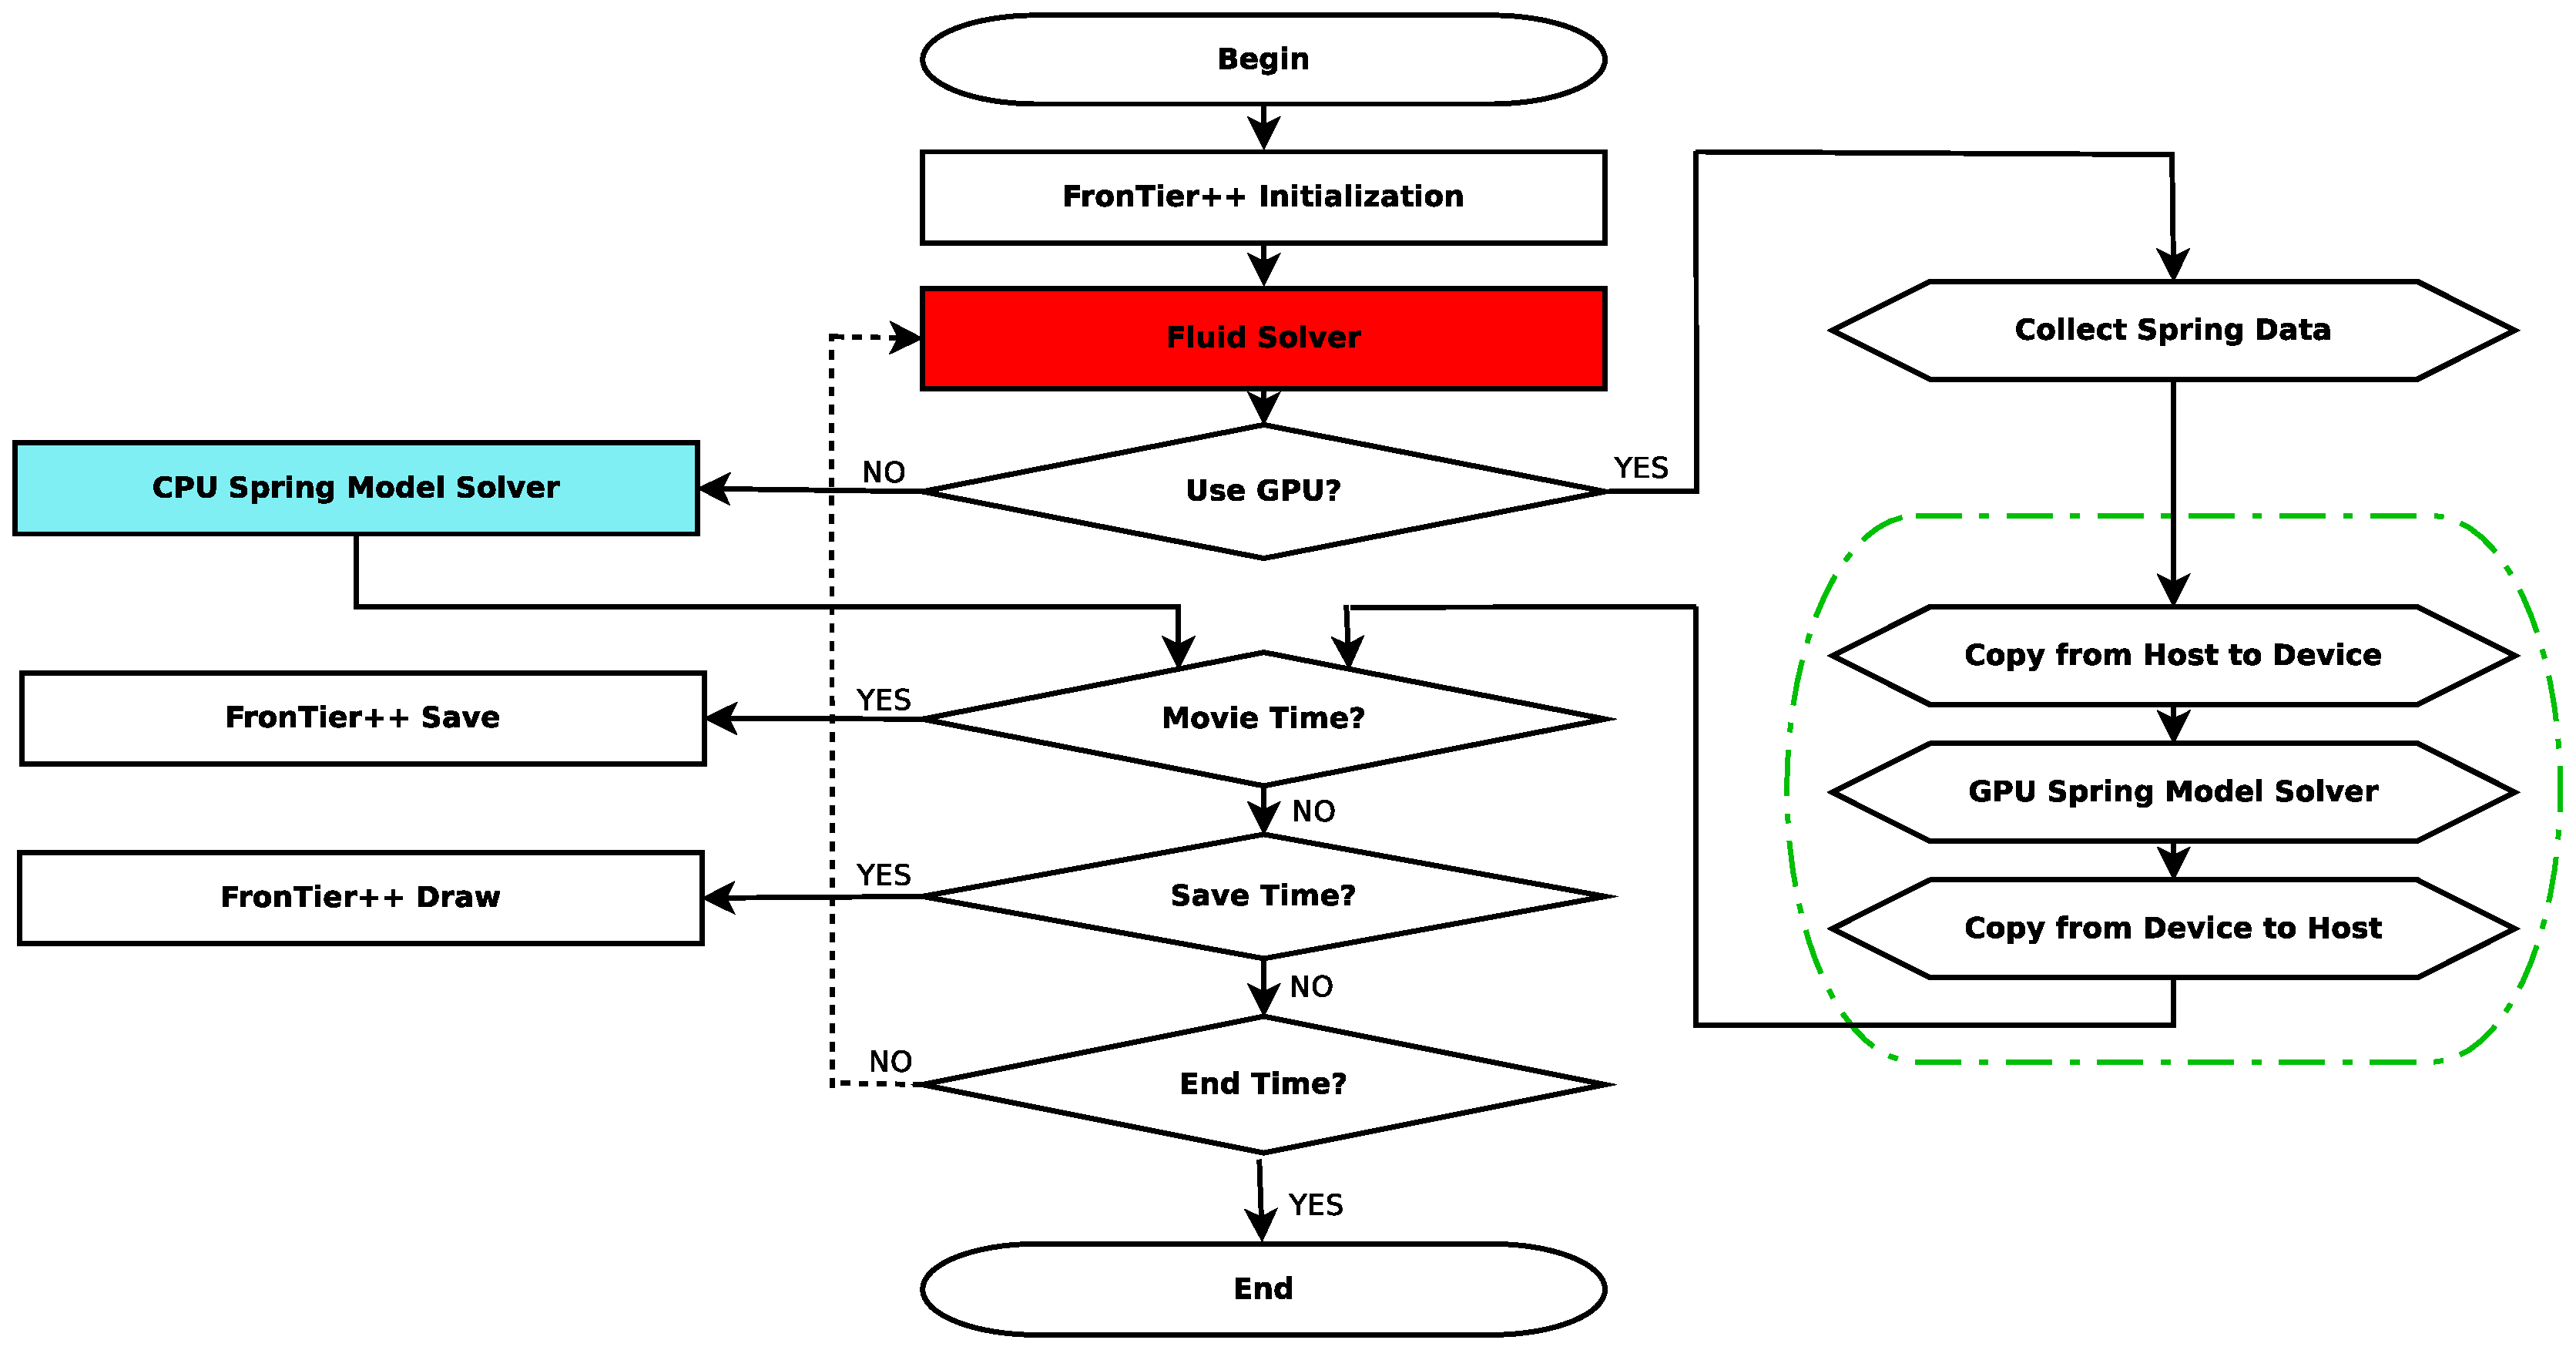
\includegraphics[width=1.0\textwidth]{figures/flowchart}
\caption{Flow chart of the complete simulation algorithm that involves
both fluid dynamics and elastic structure dynamics. The part inside the green
dash-dotted line is the work involves done by GPU.}
\label{fig:sm_flow_chart}
\end{figure}

Graphics Processing Unit (GPU) compution \cite{kirk2010programming} is to
use the GPUs together with CPUs to accelerate a general-pourpose scientific
and engineering application.
For the blue panel, we make use of the GPU technique to accelerate the
numerical calculation, i.e. the part inside the green dash-dotted line in
\Fig{sm_flow_chart}.
Solving the spring model by 4-th order Runge-Kutta method consists the
following steps:
\begin{enumerate}
\item Find the positions of all the neighbors of each spring vertex.
\item Calculate the total force on each spring vertex using Delingette method.\label{itm:2}
\item Calculate the acceleration of each vertex and update the location of
them.
\item Go to \ref{itm:2} if this is not the end of the Runge-Kutta; finish this
time step, otherwise.
\end{enumerate}
To accelerate the calculation of this part, we then shift it to the GPU
cores for massively parallel processing.
When we apply the GPU code to the complete parachute system, including both
the parachute canopy and all the suspension lines, we can achieve 16-21
$\times$ faster then pure CPU code for different types of parachutes, as
shown in \Tab{gpu_speedup}.
\begin{table*}
\centering
\begin{tabular}{cccccc}
\hline\hline
Parachute type & CPU/GPU & Time(s) & Avg time per step(s) & Speedup\\
\hline
\multirow{2}{*}{C-9} & CPU & 2805.85 & 3.39 & 1.00 \\
 & GPU & 131.90 & 0.16  & 21.2 \\
\hline
\multirow{2}{*}{G-11} & CPU & 5101.47 & 5.41 & 1.00 \\
 & GPU & 243.18 & 0.26 & 20.81 \\
\hline
\multirow{2}{*}{Intruder} & CPU & 1252.65 & 2.00 & 1.00 \\
 & GPU & 69.67 & 0.11 & 18.18 \\
\hline
\multirow{2}{*}{T-10} & CPU & 5540.02 & 5.99 & 1.00 \\
{} & GPU & 282.74 & 0.36 & 16.64\\
\hline
\multirow{2}{*}{T-11} & CPU & 6791.9 & 5.12 & 1.00 \\
{} & GPU & 352.07 & 0.29 & 17.66\\
\hline
\end{tabular}
\caption{A comparison of computational time between different parachute
types using CPU and GPU code. The speedup is calculated based on the
computing time by CPU.}
\label{tab:gpu_speedup}
\end{table*}

The solution for the red panel is to use multiple CPU cores; each CPU is in
charge of the calculation of one part of the computational domain.
The fluid computational domain is partitioned according to the computational
mesh grid, however, it is not the case for the canopy surface.
Intuitively, cutting the canopy surface through its edges is not reasonable
in the spring-mass model.
Therefore, a modified partitioning algorithm is applied which cut the canopy
surface according to the particles on it, as demonstrated in
\Fig{cpu_parallel} with $2 \times 2$ partitioning.
\begin{figure}[!ht]
\centering
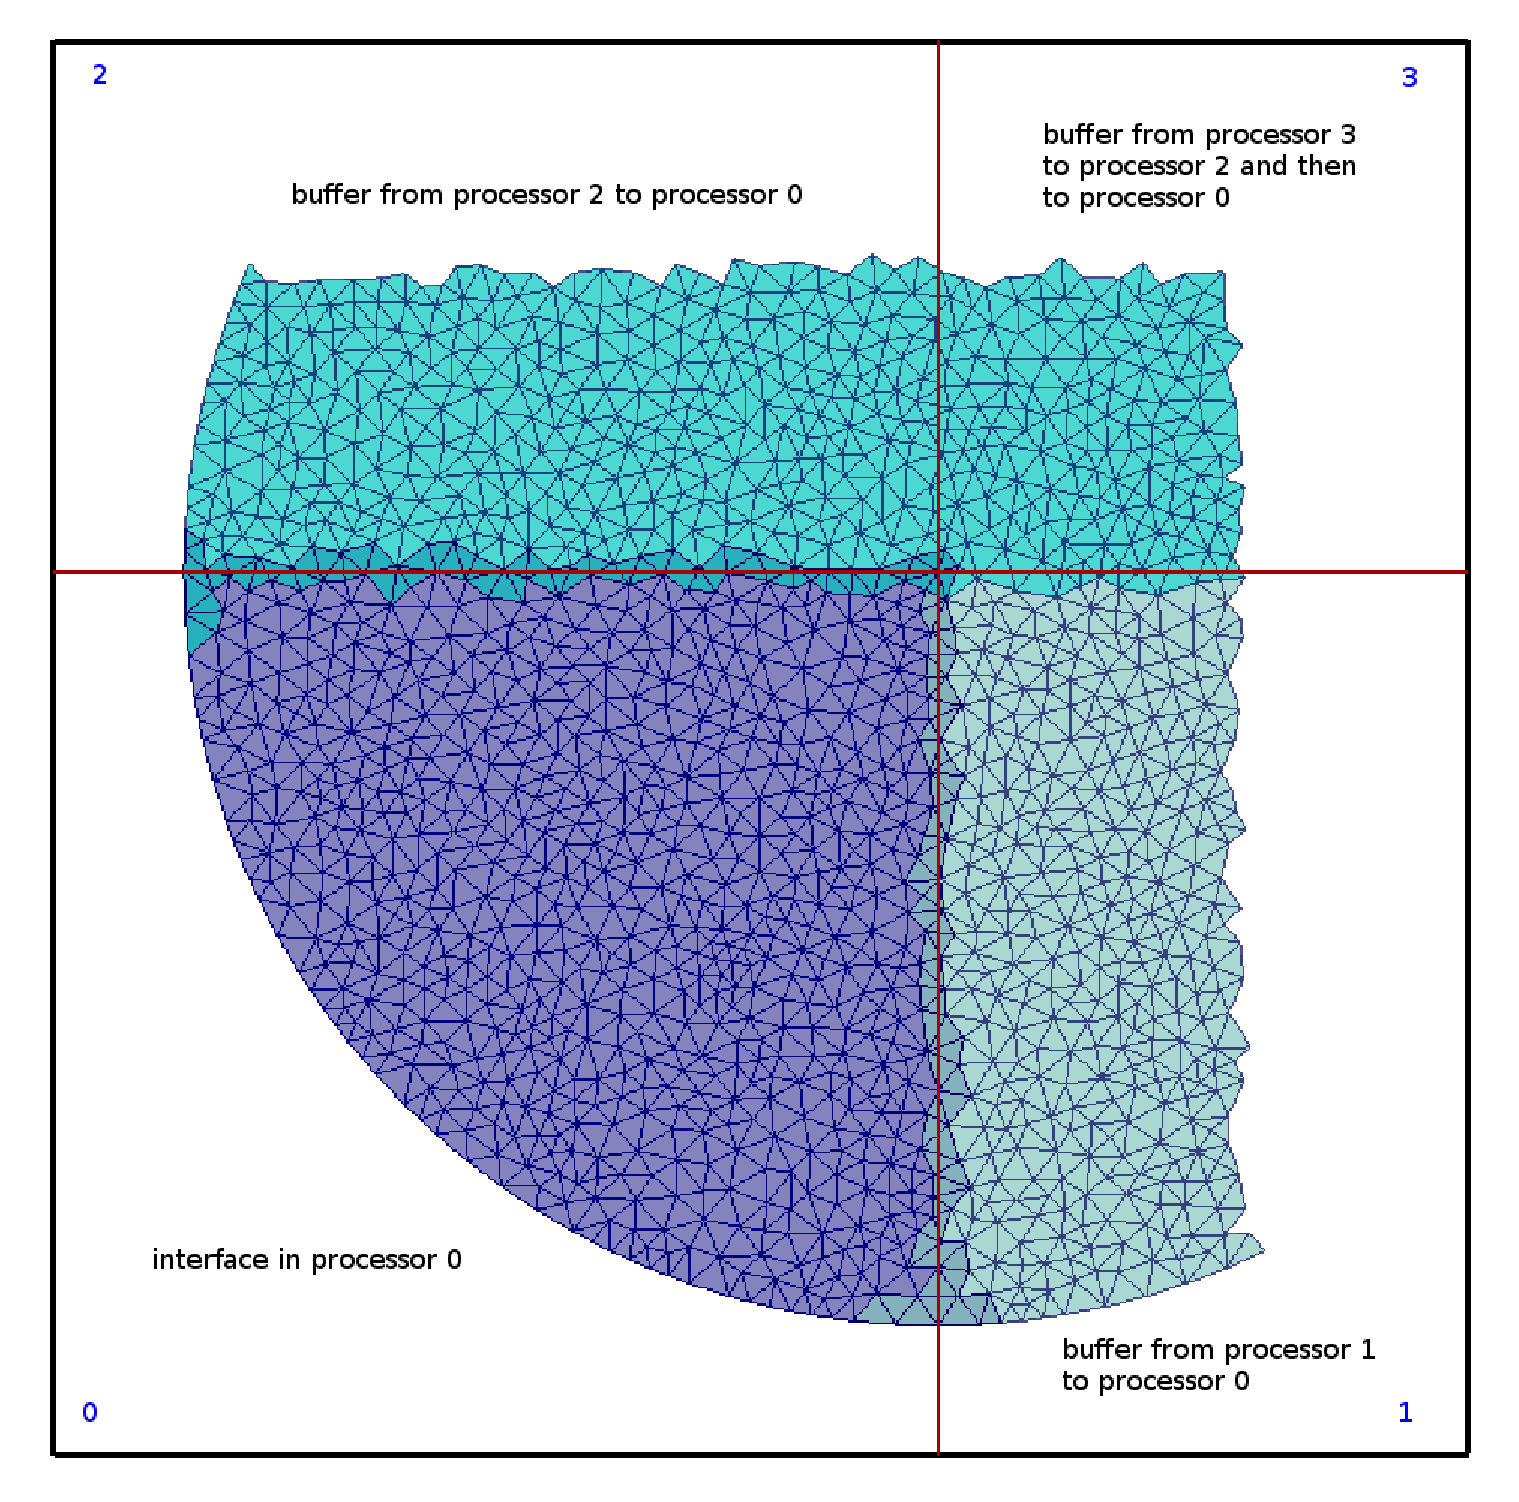
\includegraphics[width=0.66\textwidth]{figures/cpu_parallel}
\caption{A demonstration of the clipped interface in processors 0 and its
buffer interfaces from neighbor processors.}
\label{fig:cpu_parallel}
\end{figure}

The lower left part is the interface in processor 0, it received buffer
interface from two neighbor processors, 1 (lower right) and 2 (upper left).
The buffer interface provides neighbors to spring vertices that are close
to the sub-domain boundary.
Since the communication of buffer interface is done dimension by dimension,
the buffer interface from processor 2 contains part of the buffer interface
from processor 3 to processor 2.
With this partitioning algorithm, the spring-mass model work well with
multiple processors.

Furthermore, two techniques can be coupled together in the simulation of
parachute system.
\begin{enumerate}
\item Collect mass point information of the fabric structure from each
processor to the main processor.
\item Call the GPU-based spring model solver in the main processor.
\item Distrubute the updated information of each mass point to its
corresponding processor.
\end{enumerate}



\newpage
	   % Parallelization
\chapter{Conclusion and Future work}
\section{Conclusion}
\newpage




\section{Future Work}
\newpage
\newpage
 	   % Conclusion
\end{spacing}

\begin{spacing}{\singlespace}	% Bibliographies must be
				% in single spacing in an entry and
				% double spacing between entries
				% MAKE SURE THE SPACING
\bibliographystyle{plain}	% plain or ieeetr

\bibliography{refs}
\end{spacing}

%\begin{spacing}{\defaultspace}  % adjust spacing
%\input{appendix}
%\end{spacing}

\end{document}
